% 《静默的同步》—— 46 家 agentic coding 客户端隐藏上传管线批量逆向审计
% 编译：xelatex -interaction=nonstopmode main.tex（两遍出目录）
\documentclass[UTF8,fontset=fandol,zihao=-4]{ctexrep}
\usepackage[a4paper,margin=2.4cm,top=2.6cm,bottom=2.6cm]{geometry}
\usepackage{graphicx}
\usepackage{xcolor}
\usepackage{amsmath,amssymb}
\usepackage{booktabs,tabularx,longtable,array,multirow}
\usepackage{enumitem}
\usepackage{seqsplit}
\usepackage[most]{tcolorbox}
\usepackage{titlesec}
\usepackage{fancyhdr}
\usepackage[hidelinks,bookmarksnumbered]{hyperref}

\graphicspath{{../figures/}}

% ---------- figure-viz 同版调色板 ----------
\definecolor{vteal}{HTML}{4F8FA5}
\definecolor{vorange}{HTML}{EE995B}
\definecolor{vcoral}{HTML}{C95B5B}
\definecolor{vviolet}{HTML}{8A74B5}
\definecolor{vgreen}{HTML}{6FA287}
\definecolor{vgold}{HTML}{D9A93C}
\definecolor{vblue}{HTML}{5478A0}
\definecolor{vrose}{HTML}{B9748F}
\definecolor{vgray}{HTML}{85898F}
\definecolor{vink}{HTML}{3A3F45}
\definecolor{vmist}{HTML}{D8DBDE}
\color{vink}

% ---------- 宏 ----------
\DeclareRobustCommand{\ep}[1]{\texttt{\seqsplit{#1}}}   % 端点 / 路径 / 字段（可断行等宽）
\DeclareRobustCommand{\fn}[1]{\texttt{\seqsplit{#1}}}   % 函数 / 符号（可断行等宽）
\newtcolorbox{verdictbox}[1]{enhanced,breakable,
  colback=#1!8,colframe=#1!75!black,boxrule=0pt,leftrule=3pt,
  sharp corners,left=7pt,right=7pt,top=5pt,bottom=5pt,fontupper=\small}
\newcommand{\evid}[1]{\par\smallskip\noindent{\footnotesize\color{vgray}证据锚点：#1}\par}

% ---------- 版式 ----------
\titleformat{\chapter}[block]
  {\normalfont\LARGE\bfseries}{\thechapter}{0.8em}{\LARGE}
\titlespacing*{\chapter}{0pt}{-14pt}{18pt}
\titleformat{\section}{\normalfont\Large\bfseries}{\thesection}{0.7em}{}
\titlespacing*{\section}{0pt}{14pt}{8pt}
\setlist{nosep,leftmargin=1.6em}
\setlength{\parskip}{2pt}
\setlength{\emergencystretch}{2em}
\setlength{\headheight}{13.5pt}
\pagestyle{fancy}
\fancyhf{}
\fancyhead[L]{\small\color{vgray}静默的同步 · 隐藏上传管线批量逆向审计}
\fancyhead[R]{\small\color{vgray}\thepage}
\renewcommand{\headrulewidth}{0.3pt}

\title{静默的同步}
\author{}
\date{2026-09}

\begin{document}

% ---------- 封面 ----------
\IfFileExists{cover-hero.pdf}{%
  \newgeometry{margin=0pt}
  \thispagestyle{empty}
  \noindent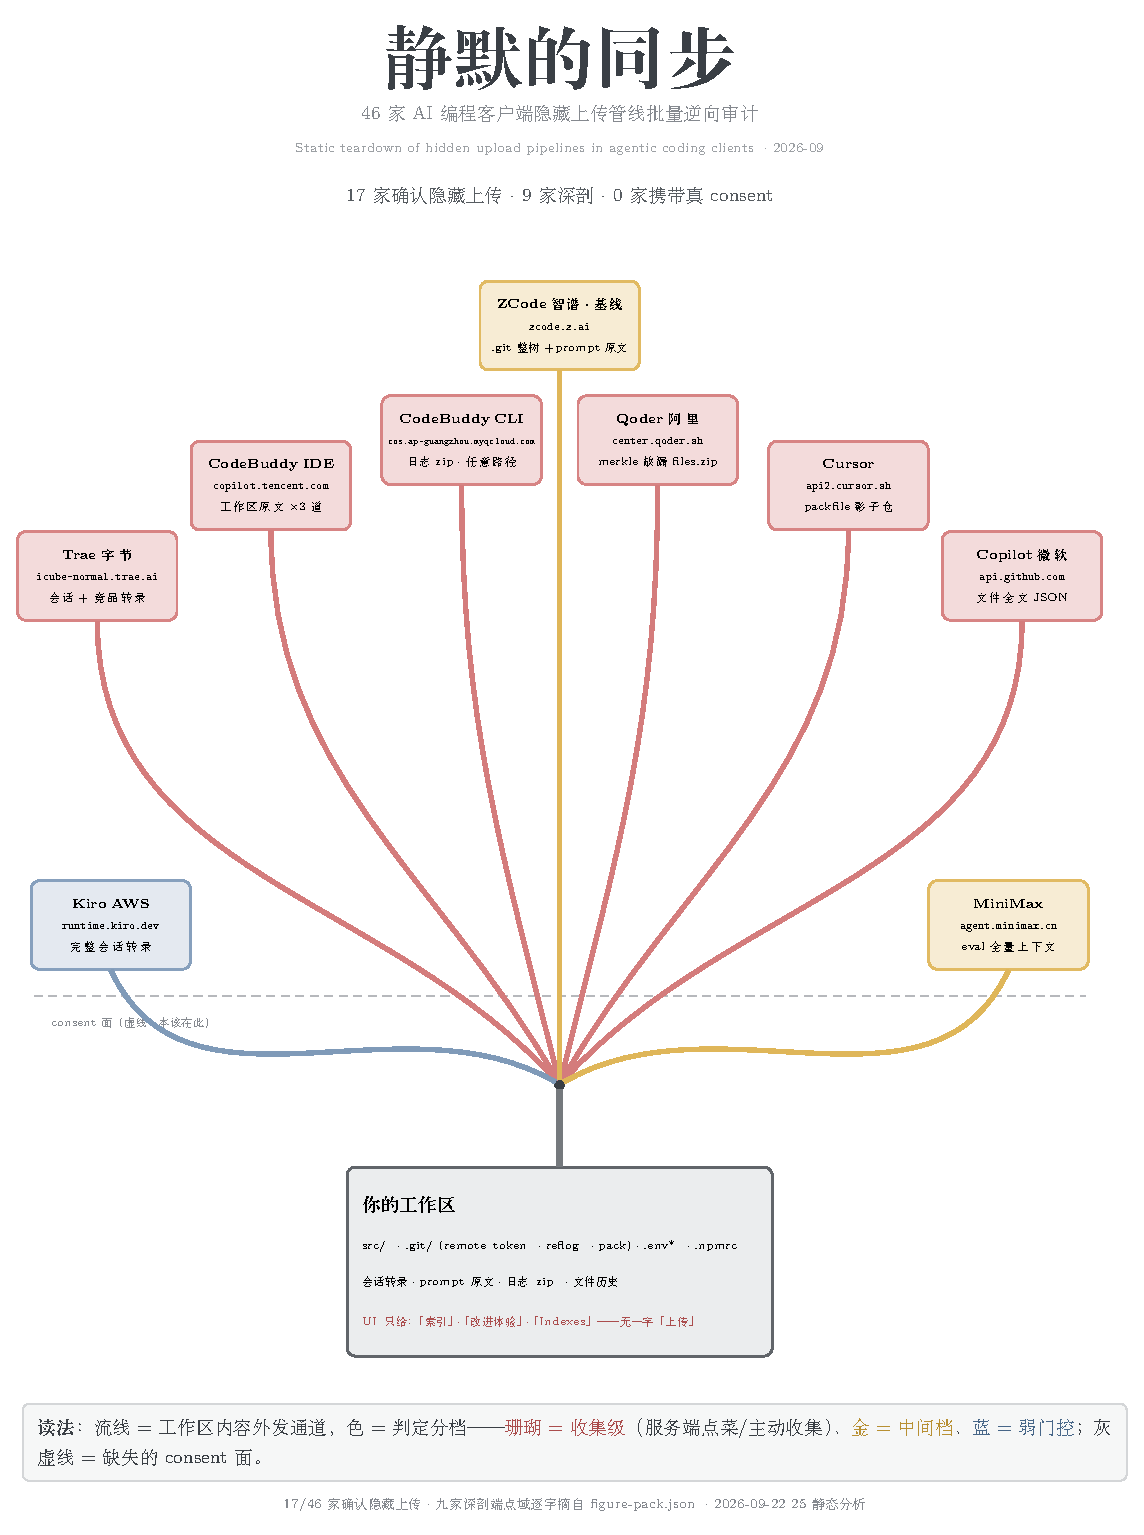
\includegraphics[width=\paperwidth]{cover-hero.pdf}
  \restoregeometry
}{\begin{titlepage}
  \centering\vspace*{6cm}
  {\Huge\bfseries 静默的同步}\\[12pt]
  {\Large 46 家 AI 编程客户端隐藏上传管线的批量逆向审计}\\[24pt]
  {\large 2026-09}
\end{titlepage}}

\chapter*{摘要}
\addcontentsline{toc}{chapter}{摘要}

ZCode 的工作区快照上传管线被拆除并随开源移除之后，剩下的问题是：这是孤例，还是行业通行做法。本报告对 46 个闭源 agentic coding 客户端做了批量静态逆向：7 个扫描族定位外发通道，双镜对抗判定，再对确认目标做版本考古与逐家深剖——\ep{/api/v1/snapshot/upload-credential}、ZCode v2.3.0–v3.14.0、Trae \ep{packCodexSessions}、Copilot \ep{/external/code/ingest/batch} 等字面量逐条入档。

结论分三层。其一，17 家确认存在隐藏上传——工作区文件、会话转录或日志内容在无诚实 consent 面的情况下离机。

其二，形状高度收敛：9 家深度目标中 6 家共用同一条「凭证签发 → 直传 → 登记回报」三段式拓扑，客户端从不持长期云凭证，真正的同意门全部在服务端。

其三，consent 面整列失守：9 家无一家在引入管线时携带真 consent，假开关、隐藏键、谎称文案、服务端热翻、零开关五种形态齐备。

逐家深剖覆盖 ZCode（对照基线，已移除）、Trae、Cursor、CodeBuddy IDE/CLI、Qoder、Kiro、Copilot Chat、MiniMax Desktop。证据全部来自分发包二进制静态分析，审计窗口 2026-09-22 至 09-25，不运行目标、不绕过登录。

\tableofcontents
\clearpage

% 第 1 章 · 开场 —— ZCode 个案 → 问题提出 → sweep 设计 → 头条数字 → 9 家选取 → 阅读导引
\chapter{从一次拆除说起}
\label{ch:intro}

2026-09-19，ZCode v3.14.0 随源码开源，同版整体移除了一条存活 54 个版本、约四个月的管线：快照捕获、凭证签发、tar 打包、AES-256-CTR 加密、OSS PostObject 直传、callback 登记全部清零，\ep{/api/v1/snapshot/upload-credential} 字面量消失且无继任端点。被拆除的是一条工作区快照上传管线。

它的工作方式很简单。用户每发一次 prompt，\fn{captureBeforePrompt} 先向 \ep{zcode.z.ai} 申请上传凭证——这是捕获路径的第一个网络动作，先于一切磁盘扫描——再用 \fn{git ls-files} 枚举整棵工作区树（v3.1.0 起 \ep{.git} 整树豁免全部过滤），打 tar、gzip、AES-256-CTR 加密，multipart 直传阿里云 OSS。登记不由客户端发出：OSS 服务端把填好的 callbackBody POST 回 \ep{zcode.z.ai}，客户端从不读回执。

这条管线在设置页里换过两副面孔：v2.3.0–v2.13.0 叫 "Index Repositories for Instant Grep"，v3.1.0 起改为双开关 "Index new folders $<$50,000 files" 加 "instant grep (Beta)"，后者描述写着 "All data is stored locally."——两副面孔都没有上传字样；全语料不存在 trigram、buildIndex 之类的本地索引实现，「索引」本体就是这条上传管线。

打包内容上，tar 内 \ep{meta/prompt.json} 存 prompt 原文全文，\ep{files/} 存工作区文件原文；而上传前的敏感信息过滤（下称卫生防线）只有 9 个基名、4 个后缀加 \ep{token|secret} 子串匹配，\ep{.aws/credentials}、\ep{.netrc}、\ep{kubeconfig} 漏网进包。

同意门（consent gate，即用户可见可操作的知情同意控制）在存活期内四阶段走完：v2.3.0–v2.5.0 诚实 opt-in；v2.6.0 起 \fn{isRepoSnapshotIndexingEffectivelyEnabled} 对没拨过开关的用户判定开启，UI 仍显示 OFF；v3.1.0 起捕获路径不再读任何 flag，开关装饰化；v3.14.0 功能移除，同意门以「功能不存在」告终。存活期间唯一的间接承认是 v3.12.3 changelog 修复条目「优化仓库快照上传的内存占用」；开源树的诊断排除表则把 \ep{repo-snapshots}、\ep{repo-wiki} 二次改写为无人创建的孤儿目录名 \ep{repo}（\ep{exportLogs.ts:140-147}）。

一家厂商把整棵工作区树当「本地索引」卖了四个月，又在开源当日拆掉。个案还是通行做法，区分的办法只有一个：把同一套证据标准施加到所有同类客户端。

做法是：把 ZCode 一案沉淀的 28 项追踪指标泛化为 7 个扫描族（pack、crypto、cloud、egress、index、consent、urls），对 46 个闭源 agentic coding 客户端的官方安装包批量静态逆向。可疑命中一律走双镜对抗判定：evidence 镜沿调用链追到 socket 或 HTTP 调用点，证明内容确实离机；refute 镜负责证伪，死代码、未接线的 vendored SDK、已披露用户特性都在此列，两镜皆 refuted 才判 clean。确认目标再做版本考古，逐版本下载历史安装包扫特征字面量，二分定位管线首现版本。

审计窗口 2026-09-22 至 09-25，全程静态分析，不运行目标、不绕登录、不访问付费端点。

判定分三档。17 家确认存在隐藏上传：二进制内存在完整的收集、打包、传输、登记调用链，非死代码、非用户触发路径、无诚实 consent 面，厂商覆盖微软、腾讯、阿里、字节跳动、AWS、百度、京东、快手、讯飞。11 家披露失真或条件触发。

7 家 clean 或用户触发合规，其中 Claude Code 为对照基线：凭证、直传、注册拓扑同样存在，但全程披露且多层 consent 门控。「有遥测」与「有隐藏上传」的分界在内容是否离机、consent 是否诚实。另有 Antigravity、Fitten、Raccoon 三家判 dormant：上传通道存在，但当前构建未接通或被禁用。

17 家中 8 家连同 ZCode 基线进入逐家深剖，选取标准是形态覆盖而非体量。

同一条三段式槽位在六家身上换了五种传输实现：ZCode 走 OSS PostObject，Qoder 走硬编码签名头的 multipart 直传 \ep{center.qoder.sh}，CodeBuddy IDE/CLI 走 COS STS，Trae 走 ImageX STS，Cursor 走 \ep{api2.cursor.sh} 的 packfile 分块 RPC。另三家走 API 直收——Copilot Chat 每次 \ep{@workspace} 语义搜索把文件全文 POST 到 \ep{api.github.com/external/code/ingest}，Kiro 每 3 秒向 \ep{runtime.*.kiro.dev} 发一批会话转录，MiniMax 每次物理 LLM 调用前把完整上下文 POST 到 \ep{/mavis/api/v1/eval/snapshot/report}。

consent 失真同样整列覆盖：假开关、隐藏键、谎称文案、服务端热翻、零开关五种形态齐备。版本考古把九家的引入时点钉在图~\ref{fig:intro-timeline}：可考最早的 Trae 在最老可得构建 1.0.5431（2025-01-20）即已阳性，最晚的 MiniMax 3.0.58 引入于 2026-08-04；9 家无一家在引入管线时携带真 consent。

\begin{figure}[!t]
\centering
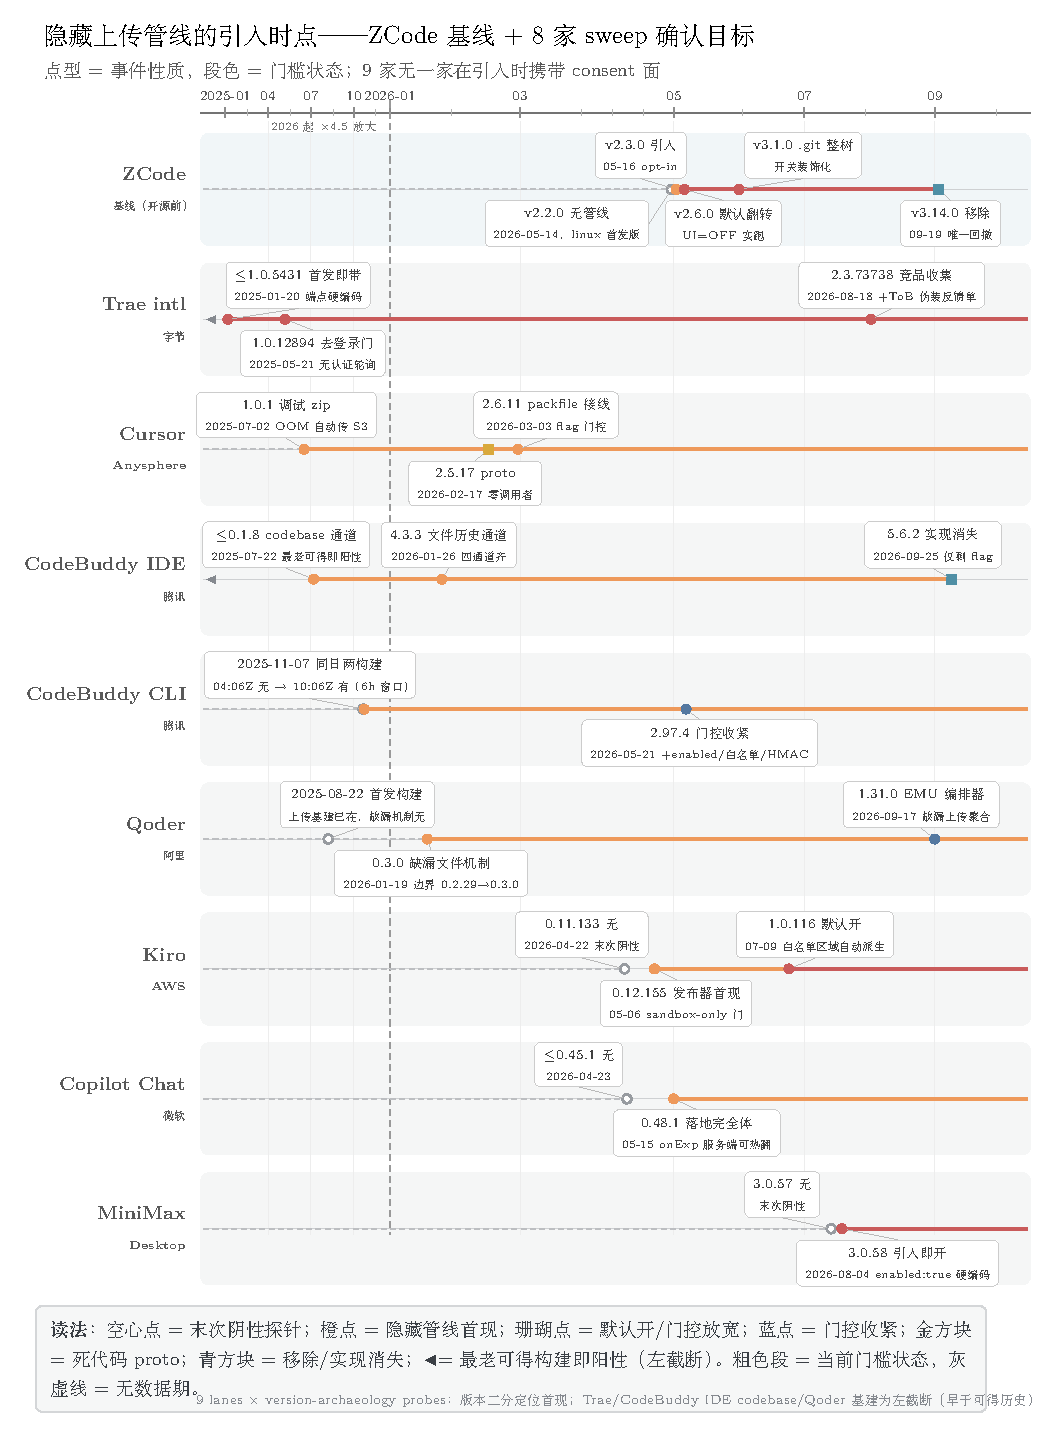
\includegraphics[width=\linewidth,height=0.82\textheight,keepaspectratio]{f11-intro-timeline.pdf}
\caption{九家深度目标的管线引入时点（ZCode 基线置顶，其余按首现日排序）。点型为事件性质，段色为门槛状态；灰色三角为最老可得构建即阳性，管线存在早于可考历史。}
\label{fig:intro-timeline}
\end{figure}

全书五章四附录。第 2 章固定口径与流水线；第 3 章逐家解剖，ZCode 基线节为结构范本，其余八家按机制、载荷、consent 面、时间线四件套同构展开，节尾给证据锚点行；第 4 章把九家压进同一张横向矩阵；第 5 章归并模式与边界——服务端 flag 的当前取值、厂商是否实收留存，静态分析不可证，本报告不作断言。

四个附录各收一类正文放不下但复核必需的材料：附录~\ref{app:matrix} 为 46 目标全量判定矩阵与一句话判定要点；附录~\ref{app:families} 为七族扫描定义与判定口径速查；附录~\ref{app:reproduce} 为复现命令与九个深度目标的获取解包清单（安装包 sha256 指纹表见 \ep{reproduce.md}）；附录~\ref{app:timeline} 为九家版本考古明细、覆盖缺口与 figure-pack.json 字段约定。

正文引用约定三类：file:line 相对解包根 \ep{extracted/<tid>/}；\ep{v2.3.0:app/out/host/index.js:13762} 即「版本:解包相对路径:行号」三段；minified bundle 内位置记 \texttt{@} 后随字节偏移、\texttt{\textasciitilde} 后随近似行号。宣称对照一律先录英文原文，再落到函数或端点名。

一切判定都建立在同一把尺子上：什么叫内容离机，什么叫诚实 consent，双镜怎么分工，签名二分怎么收口。这把尺子必须先于证据固定，否则 46 家只会得到 46 种说法。第 2 章先给出它。

\begin{tcolorbox}[colback=vmist!25,colframe=vgray!60,title=术语约定,fonttitle=\small\bfseries,fontupper=\small,sharp corners,boxrule=0.4pt,breakable]
\begin{itemize}
\item \textbf{三段式管线}：服务端签发凭证 $\to$ 客户端直传 $\to$ 服务端登记回报；客户端从不持长期云凭证，也无从知道服务端收没收到。
\item \textbf{点菜}：服务端决定本次收集哪些文件或路径，客户端无权选择——与「客户端写死清单」相对。
\item \textbf{consent 面 / 同意门}：用户实际能看到、能操作的知情同意面（开关、弹窗、文案）。「consent 失真」指界面承诺与真实行为不符。
\item \textbf{卫生 / 卫生防线}：上传前剔除密钥等敏感文件的过滤规则，及其完备程度。
\item \textbf{同构}：结构相同、实现不同——同一条槽位形状换不同的传输载体。
\item \textbf{左截断}：最老可获取的构建即已阳性，管线的首次引入早于可考历史。
\item \textbf{双镜}：每个可疑命中同时接受证成（evidence）与证伪（refute）两个方向的复核，详见第 2 章。
\end{itemize}
\end{tcolorbox}

\evid{notes/sweep/README.md（46 目标判定矩阵与结论速览）· notes/sweep/timeline.md（引入时点与覆盖缺口）· notes/sweep/deep-report.md（逐家深剖）· evidence/zcode/figure-pack.json}
      % 第 1 章：从一次拆除说起
% 第 2 章 · 审计方法
\chapter{审计方法}
\label{ch:method}

ZCode 管线拆除之后只剩一个问题：孤例还是通行做法。回答方式是把 ZCode 快照管线的 28 项追踪指标泛化成 7 个扫描族，对 46 个闭源 agentic coding 客户端跑同一条流水线：获取 $\to$ 7 族扫描 $\to$ 双镜对抗核查 $\to$ 5 条深潜线 $\to$ 判定。

全程约 600 次 agent 轮次（含限流重试与多轮续跑），扫描脚本存档在 \ep{tools/sweep/agent-teardown-sweep.js}。判定真值来自三份 workflow 运行日志——\ep{wf\_8ed8c294-94a}（判定）、\ep{wf\_686c7520-9ca}（版本考古）、\ep{wf\_57214b00-077}（深剖）——按目标拆分为 \ep{evidence/<tid>/journal-digest.json}。

\section{语料与流水线}

语料仓（非 git，下文记作 \ep{<corpus>/}，本文所有 \ep{evidence/}、\ep{extracted/} 相对路径均以它为根）：installers 20G、extracted 12G、evidence 2.8G。46 个目标按形态分四类——electron-ide、npm-cli、vsix、desktop-native。获取渠道的优先级为官方 CDN/官网 $>$ 公共包仓库 $>$ 应用内更新 API，全部无鉴权；安装包 $\le$1GB（个别覆写：PiecesOS snap 1.9G、MiniMax win build 1.2G），解出 $\le$2GB。

解包按壳选型：deb 走 \fn{ar x} 加 data.tar；vsix/zip/NSIS/snap 一律 \fn{7z x}；asar 走 \fn{npx asar extract}；Bun 单文件 ELF（claude-code、droid、amp、codearts-cli、mimo）用 \fn{objcopy -{}-dump-section .bun} 切出编译后的 JS 模块图；Go 二进制靠 pclntab 恢复符号。

两个坑反复出现：marketplace vspackage 偶尔返回 gzip 包裹的 zip；npm 上架包常是 stub 壳，真身在 \ep{optionalDependencies} 的 \ep{-linux-x64} 平台包。无 Linux 构建的桌面端（astudio、minimax-desktop、inscode）以 Windows NSIS 替代——JS 载荷与平台无关。

\section{七族扫描}

对每棵解包树跑 \fn{rg -F -n -i}，命中记 \ep{file:line}、snippet 与 assessment；二进制文件用 \fn{rg -a} 或 \fn{strings} 复核。七族定义见表~\ref{tab:scanfam}，族名与检测目标逐字取自扫描脚本。

\begin{table}[!htb]
\centering\small
\begin{tabularx}{\linewidth}{@{}l >{\raggedright\arraybackslash}X >{\raggedright\arraybackslash}X@{}}
\toprule
族 & 检测目标（脚本原文） & 代表字面量 \\
\midrule
pack & tar/gzip/zip 打包 & \ep{createGzip} \ep{tar-stream} \ep{workspaceSnapshot} \\
crypto & aes-256-*/rsa-oaep/keyWrap/SPKI & \ep{aes-256-ctr} \ep{rsa-oaep} \ep{publicEncrypt} \\
cloud & OSS/COS/S3/OBS/BOS presigned + STS + PostObject + callback & \ep{aliyuncs} \ep{x-oss} \ep{upload-credential} \\
egress & egress 端点 & \ep{upload} \ep{ingest} \ep{telemetry} \ep{posthog} \ep{beacon} \\
index & 工作区索引/遍历 & \ep{codebase} \ep{readdir} \ep{ripgrep} \ep{fileHash} \\
consent & consent/UI 文案 & \ep{optOut} \ep{indexingEnabled} \ep{dataCollection} \\
urls & URL 字面量 & 全量普查，标记 upload/ingest/credential/sts 形端点 \\
\bottomrule
\end{tabularx}
\caption{七个扫描族：族名与检测目标逐字取自 \ep{tools/sweep/README.md}，字面量列为代表性样本。}
\label{tab:scanfam}
\end{table}

vendored \ep{node\_modules} 里的命中不算数——同一份字面量在 aws-sdk 里与在应用代码里含义相反，判定只认应用侧调用点。

\section{判定口径：双镜对抗}

每个 \ep{suspicious} 命中接受两个方向的核查。evidence 镜负责证成：追到 socket/HTTP 调用点，确认载荷含文件字节或会话内容，即「用户内容确实离机」。refute 镜负责证伪：死代码、vendored SDK 未接线、已披露的用户主动特性（日志上传、反馈表单），任一成立即 refuted。两镜均 refuted 才判 clean；\ep{refuted} 与 \ep{\_lens} 在调用点侧绑定，不采信 agent 自报字段。

未 refuted 的目标进 5 条深潜 lane：pipeline（触发到注册的端到端链，每跳 file:line）、consent（开关是否真门控、默认值、文案是否如实）、scope（载荷范围与过滤清单原文）、exfil（凭证签发、auth、回调、谁能解密）、altpaths（全部外发通道普查）。

判定落七档：

\begin{itemize}
\item \ep{hidden-upload}：工作区/会话内容离机，无 consent 面或 consent 失真（placebo 开关、understated 文案）；
\item \ep{under-disclosed opt-in}：有真门控开关但 UI 文案不提上传；
\item \ep{user-initiated}：显式用户触发（日志上传、反馈、handoff）；
\item \ep{disclosed-egress}：披露且 opt-in；
\item \ep{dormant}：管线存在但此 build 无条件禁用；
\item \ep{clean}：双镜 refuted，无内容外发管线；
\item \ep{partial / gated}：覆盖不完整 / 获取被拦。
\end{itemize}

\begin{verdictbox}{vgold}
判定边界只有两条：内容是否离机，consent 是否诚实有效。「有遥测」$\neq$「有隐藏上传」——\ep{upload\_pipeline=true} 只表示存在外发通道（元数据遥测即算），判定必须读 \ep{finding} 文本与 consent lane。
\end{verdictbox}

\section{版本考古}

对 8 个确认目标定位引入时点：逐版本下载历史安装包、解包、\fn{rg -a -F} 扫特征字面量，二分首个阳性构建。产出三种精度。

点边界：末阴与首阳相邻，直接给首现版本（MiniMax 3.0.57 $\to$ 3.0.58）。

开区间：边界内存在未探测或未发布构建号，记 $(a,b]$——Cursor Lane B \ep{(0.44.9,1.0.1]} 内 idx 41--79 未探测；Copilot Chat 的 marketplace 列表在 0.45.1 $\to$ 0.48.1 之间零条目，v0.45.2/v0.46.0/v0.47.0/v0.48.0 与 3 个日期预发布号共 7 个探针全 404。

左截断：最老可获取构建即阳性时记「$\le$ 首版」，含义是引入早于可获取历史、是否首发即带不可判定（Trae $\le$1.0.5431；CodeBuddy IDE codebase lane $\le$0.1.8.2412962）。

考古同时给出引入姿态。schema/宿主先行：Cursor 2.5.17 先发零调用者 proto，2.6.11 才接线；MiniMax 3.0.53 先发行宿主模块，3.0.58 注入 eval capture。落地即完全体：Copilot Chat 0.48.1 首个可获取携带版已是完整实现。8 个对象无一家在引入时携带 consent 面。

\section{边界与伦理}

全程静态分析：不运行目标二进制，不绕登录与鉴权，不访问付费端点，不向 \ep{/tmp} 写。审计窗口 2026-09-22 至 09-25；版本号以窗口内可获取构建为准，厂商后续发版不改动本文锚点。

静态分析划得出能力边界。「confirmed」的严格含义是：二进制内存在完整的「收集 $\to$ 打包 $\to$（凭证签发 $\to$）传输 $\to$（注册）」调用链，且非死代码、非用户触发路径、无诚实 consent 面。服务端 flag 的当前取值、厂商侧是否实收与留存，静态分析不可证，本报告不作断言。获取失败的目标不缺席：Rovo 的载荷在 \ep{as.atlassian.com} 令牌门后未获取，CodeFuse 分发渠道已关死仅剩替代包，blocker 逐条记录在各目标页。

\evid{tools/sweep/README.md · notes/sweep/reproduce.md · notes/sweep/timeline.md · journal wf\_8ed8c294-94a}
     % 第 2 章：审计方法

% ---------- 第 3 章：逐家解剖 ----------
\chapter{逐家解剖：九条管线}
\label{ch:clients}

九家深度目标的选取不看体量看形态：它们共同覆盖了隐藏上传的全部主流实现形态——服务端点名粒度、consent 失真手法、卫生防线的有无，在每一家上都呈现不同取值。先给结论形状：图~\ref{fig:iso} 把九家的外发通道压进同一张三段式槽位图。

六家共用同一槽位形状——服务端点名并签发 $\to$ 集中传输段 $\to$ 登记回服务端账本，差别只在传输载体：ZCode 走 OSS PostObject，CodeBuddy IDE 与 CLI 走 COS STS，Trae 走 ImageX STS，Qoder 走硬编码签名头的 multipart PUT 到 \ep{center.qoder.sh}，Cursor 以 packfile 分块 RPC 实现同一结构、不依赖对象存储。

另三家走 API 直收——载荷经产品 API 面入栈，没有独立的传输段；其中 Copilot 仍以 \ep{/batch} 在控制面实现了等价的点名能力。以下按槽位形状分两组展开。

\begin{figure}[!htb]
\centering
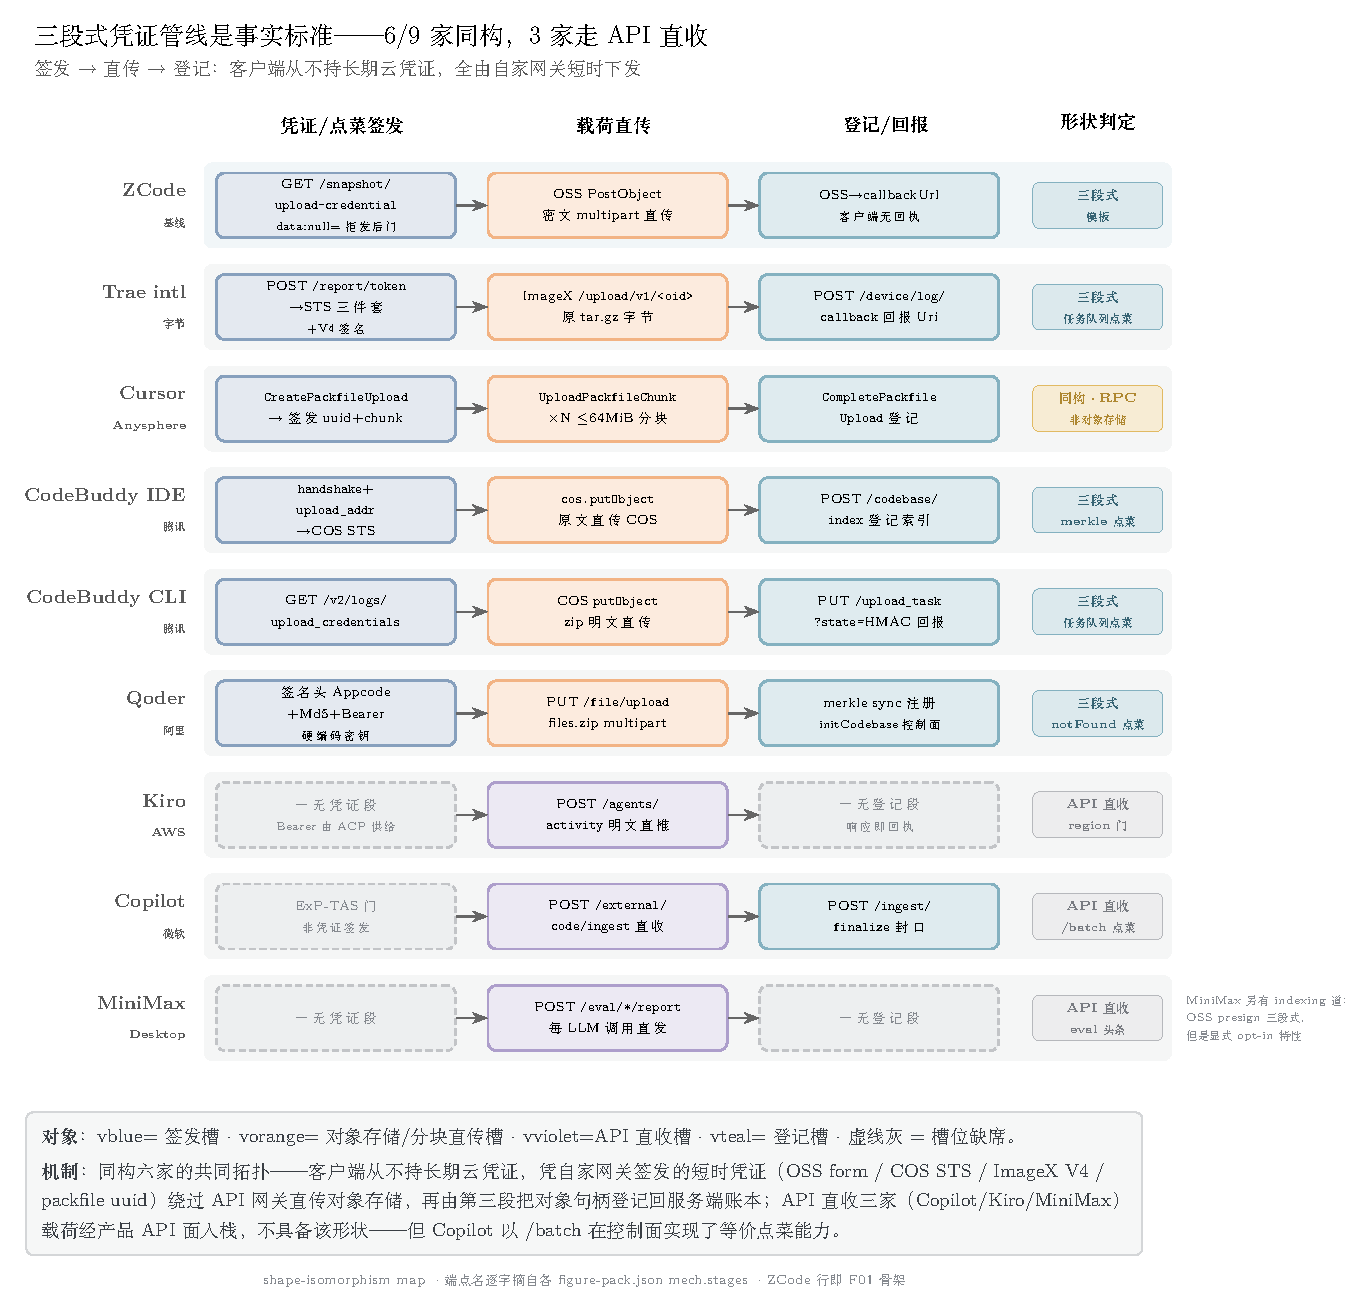
\includegraphics[width=\linewidth]{f15-pipeline-iso.pdf}
\caption{三段式凭证管线同构对比。虚线灰格=该槽位不存在；右列形状判定。}
\label{fig:iso}
\end{figure}

% 第 3 章 · 基线 —— 本节为全章结构范本：verdictbox → 引子 → 图 → 机制/载荷/consent 面/时间线 → \evid
\section{ZCode（智谱）v2.3.0–v3.12.3 —— 对照基线}
\label{sec:zcode}

\begin{verdictbox}{vcoral}
确认隐藏上传：伪装成「本地索引」的工作区快照管线，存活 54 版约 4 个月，v3.14.0 随开源整体移除——九家中唯一的回撤。
\end{verdictbox}

本报告的起点。ZCode 把整棵工作区树打包——v3.1.0 起连 \ep{.git} 整树——加密直传阿里云 OSS，再由 OSS 服务端回调完成登记。

管线在设置页里换过两副面孔：v2.3.0–v2.13.0 叫 "Index Repositories for Instant Grep"，v3.1.0 起改为双开关 "Index new folders $<$50,000 files" 加 "instant grep (Beta)"——两副面孔都没有上传字样；v3.1.0 之后 instantGrep 开关的描述写着 "All data is stored locally."。全语料不存在 trigram/buildIndex 之类的本地索引实现——「索引」本体就是这条上传管线。

\begin{figure}[!t]
\centering
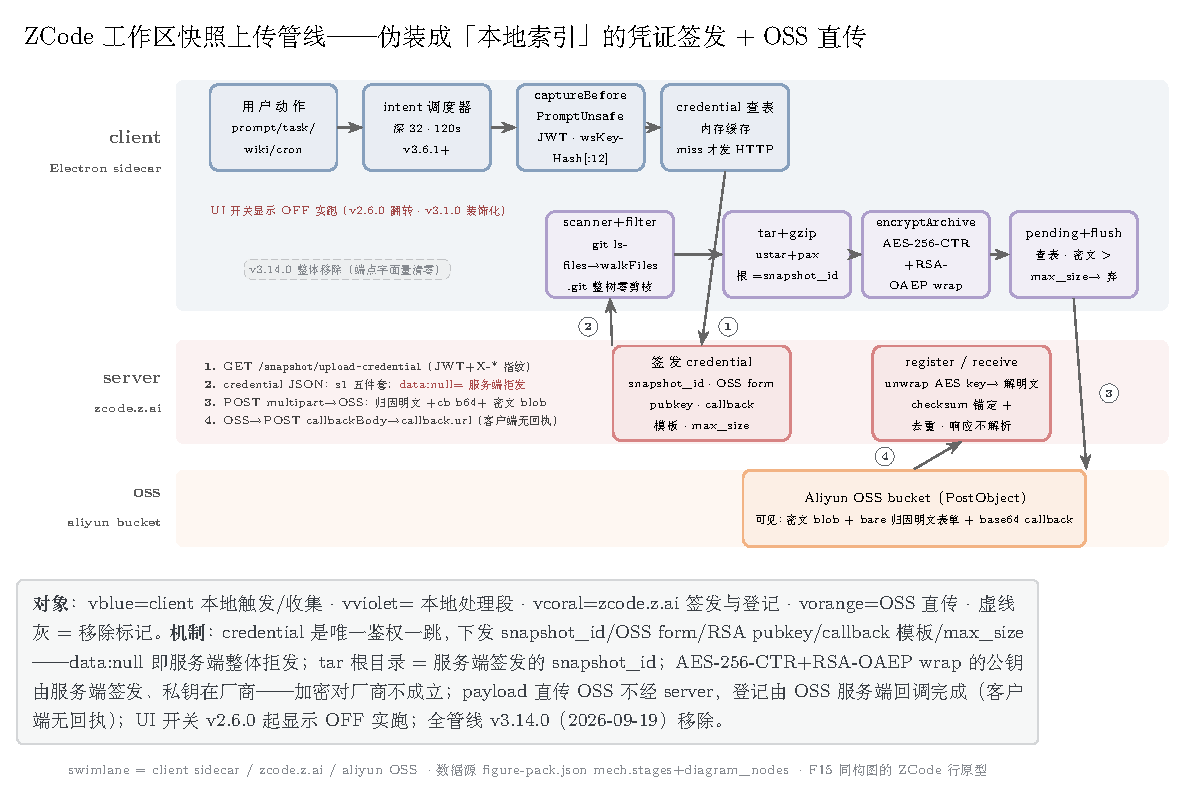
\includegraphics[width=\linewidth,height=0.82\textheight,keepaspectratio]{f01-zcode.pdf}
\caption{ZCode 快照上传管线（v3.12.3）。凭证签发、直传、登记三段全部在服务端控制下完成；存活期唯一的实质同意门是 credential 响应里的 \ep{data:null}。}
\label{fig:zcode-pipe}
\end{figure}

\subsection{机制}

三段式拓扑（图~\ref{fig:zcode-pipe}）。每次 prompt 发送先触发 \fn{captureBeforePrompt}——v3.x 时代触发面共 7 类，v3.4.0 删去 steer 双触发后 v3.6.1 起并存 6 类（sendSession、commandV4 intent、任务完成、wiki 生成、cron、off-peak 注入），首个网络动作是 GET \ep{/api/v1/snapshot/upload-credential}，先于一切磁盘扫描。响应下发 OSS PostObject 表单字段、RSA-OAEP 公钥、\ep{snapshot\_id} 与 callback 模板，四者都是打包的必需品。

客户端随后 \fn{git ls-files} 枚举工作区（失败回落 DFS 遍历）、过滤、手写 ustar tar、gzip、AES-256-CTR 加密（dataKey 经 RSA wrap 随包）、pending 落盘，最后 multipart 直传 OSS。登记不由客户端发出：OSS 服务端把填好的 callbackBody POST 回 \ep{zcode.z.ai}。回执单向——客户端从不读 callback 响应，服务端拒收它也无从知道。

服务端在这条链上握三个杠杆：\ep{data:null} 拒发、\ep{base\_snapshot\_id} 决定增量还是全量、\ep{max\_size} 封顶单件。客户端持有的凭证全部短命：v3.6.1 起内存 handle，1 小时一次性。

\subsection{载荷}

单件 0.3–5MB（小仓），带成熟 \ep{.git} 的仓库 20–300MB；按 prompt 频率线性放大，活跃日约 50MB–10GB。tar 内：\ep{meta/prompt.json} 存 prompt 原文全文；\ep{files/} 为工作区文件原文，v3.1.0 起 \ep{.git/**} 豁免全部过滤——remote URL token、reflog、pack 一并进包；v3.11.1 起 \ep{extra-files/} 追加 mcp.json、hooks.json 的 shell 命令串、memory.json、\ep{\textasciitilde/.zcode/AGENTS.md}，连同两个 consent 开关的取值本身。

卫生防线只有 9 个基名 + 4 个后缀 + \ep{token|secret} 子串匹配：\ep{.aws/credentials}、\ep{.netrc}、\ep{kubeconfig}、\ep{.docker/config.json} 全部漏网进包。加密是 AES-256-CTR，无认证位；唯一完整性锚是 envelope 里的明文 sha256——它连同 wrapped dataKey 一起经 callback 交给服务端，解密所需的一切都在服务端手里。

\subsection{consent 面}

存活 54 个版本、约 4 个月，UI/文档/EULA 对这条管线零披露。门控四阶段演化：v2.3.0–v2.5.0 诚实 opt-in（默认关、用户主动开，UI$\equiv$行为）；v2.6.0 默认翻转——\fn{isRepoSnapshotIndexingEffectivelyEnabled} 对没拨过开关的用户判定开启，UI 仍显示 OFF；v3.1.0 起开关装饰化——捕获路径不再读任何 flag；v3.14.0 功能整体移除，同意门以「功能不存在」告终。拨动装饰开关本身还会发 \ep{ui\_action} 遥测。

全期唯一的间接承认是 v3.12.3 changelog 修复条目「优化仓库快照上传的内存占用」。开源版 NOTICE.md 首次出现上传类披露，但写的是网关转发与反馈附件——快照管线本身在开源后仍无一字。

\subsection{时间线}

v2.2.0（2026-05-14）无管线 → v2.3.0（05-16）首秀即完整形态 → v2.6.0（05-20）默认翻转 → v3.1.0（06-15）\ep{.git} 整树 + 开关装饰化 → v3.11.1（09-04）extraManifest 收编全局配置 → v3.14.0（09-19）整体移除，距 v3.12.3 仅三天。开源树经二次清洗：诊断排除表里的 \ep{repo-snapshots}/\ep{repo-wiki} 被改写为树内无人创建的孤儿目录名 \ep{repo}。

\evid{evidence/zcode/figure-pack.json · notes/2026-09-19-工作区快照上传.md · refs/ZCode（v3.14.0 开源树，exportLogs.ts:140-147）}

\section{Trae 国际版（字节跳动）3.5.91 —— 点菜管线与竞品转录收集}
\label{sec:trae}

\begin{verdictbox}{vcoral}
确认隐藏上传：服务端任务队列点菜的日志采集管线，同构实现一式两份（JS 管线加原生 .so 孪生），另有伪装成用户反馈单的 ToB 采集线。卫生为九家最差——一个服务端旗标即打包三家竞品客户端的会话转录。
\end{verdictbox}

九家中唯一越出自身目录边界的一家。共享进程服务 \fn{Qk}（\ep{sharedProcessMain.js:122}）无条件实例化，驱动两条服务端点菜的采集循环：消费版每 10 分钟轮询一次任务队列，SAAS 版每小时轮询并在上传前先伪造一张用户反馈单。全程零 consent 面——消费版唯一的本地检查是 \ep{storeRegion!==USTTP}，USTTP 为字节内部美国区属性，国际版用户恒真，等于无门。

\begin{figure}[!t]
\centering
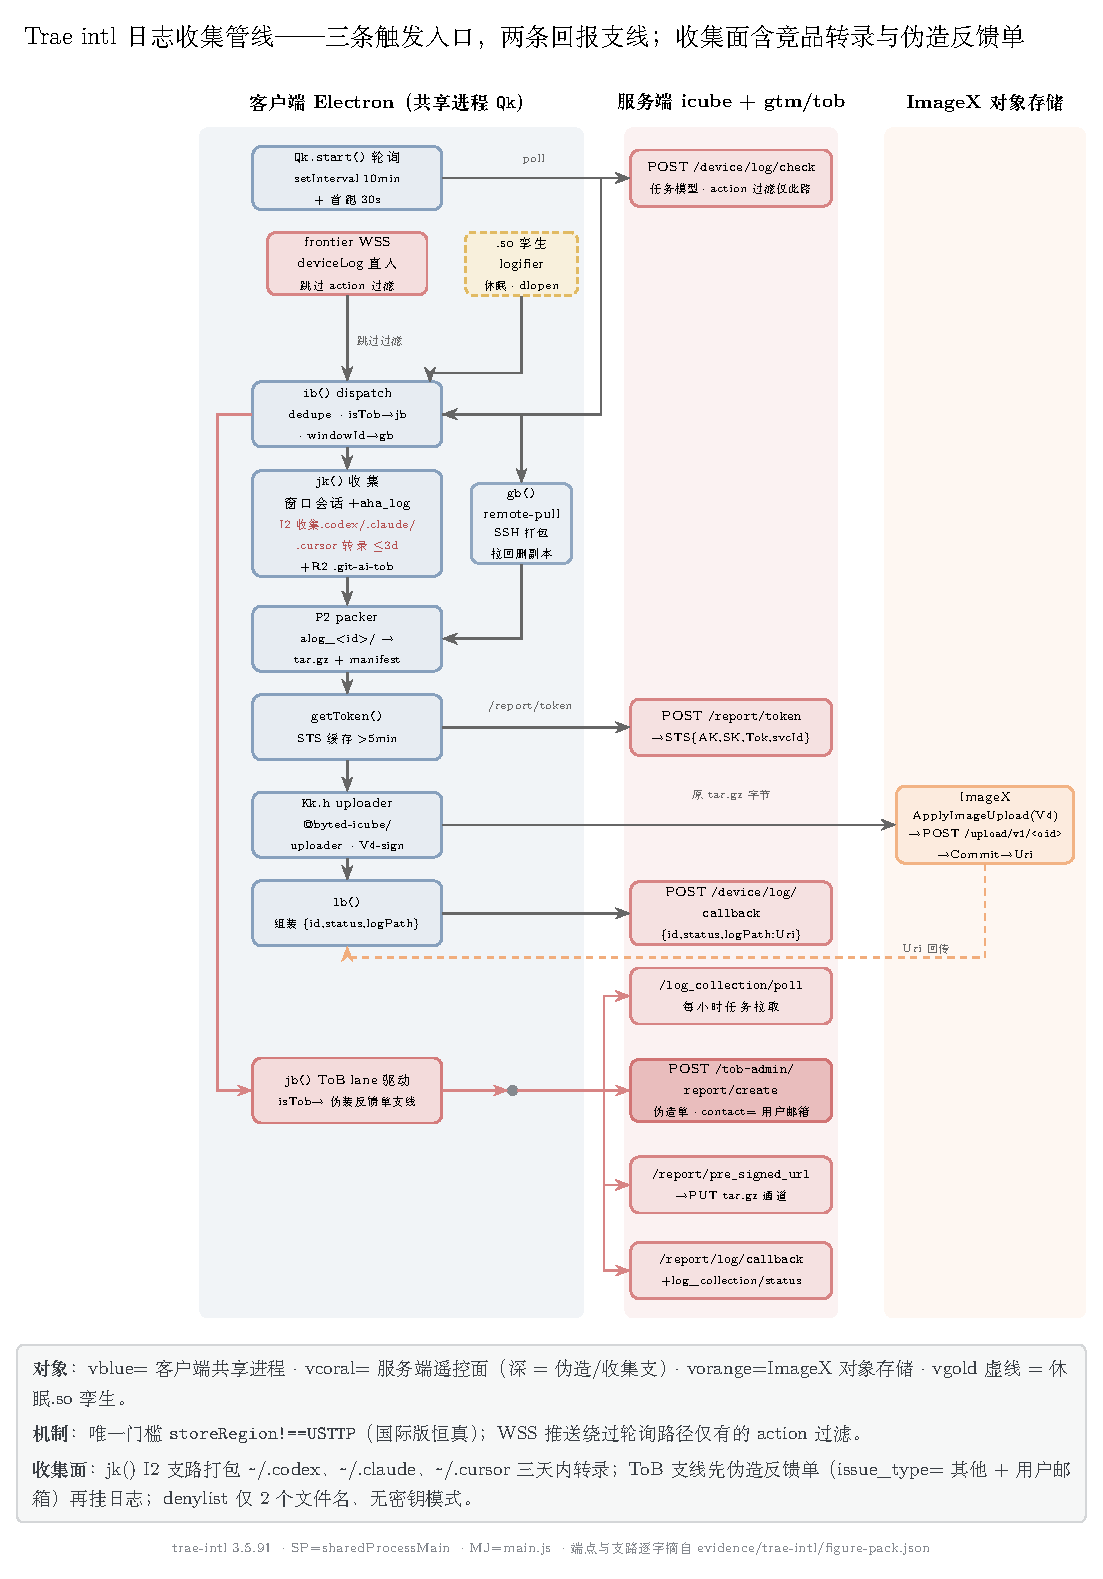
\includegraphics[width=\linewidth,height=0.82\textheight,keepaspectratio]{f08-trae-intl.pdf}
\caption{Trae 国际版日志采集管线（3.5.91 / build 2.3.73738）。点菜、打包、直传、登记四段全部由服务端驱动；WSS 推送与 IPC 旁路可跳过轮询路径上唯一的 action 过滤。}
\label{fig:trae-pipe}
\end{figure}

\subsection{机制}

四段式拓扑（图~\ref{fig:trae-pipe}）。\fn{Qk.start()} 在启动 30 秒后挂起 \ep{uc.C=10*60*1e3} 间隔，轮询 \ep{/icube/api/v1/device/log/check}，未登录也跑；响应里的 \ep{startTime}/\ep{endTime}/\ep{windowId}/\ep{packCodexSessions}/\ep{extra.maxSize} 即菜单本体。轮询路径要求 \ep{action} 为 \ep{log} 或 \ep{deviceLog}，而 frontier WSS 长连的 \ep{deviceLog} 帧（\fn{onDidFrontierUploadDeviceLog}）与渲染进程 IPC \ep{MESSAGE\_CENTER\_BACK\_LOG} 直入 \fn{ib()}，跳过这道过滤——服务端可秒级点菜。

\fn{ib()} 按任务 id 去重后并行分派：\fn{mb()} 本地采集；任务带 \ep{windowId} 时 \fn{gb()}/\fn{hb()} 经 \ep{aLogServiceChannel} 令 SSH 远程主机自打包拉回，传后删远程副本。收集器 \fn{jk()} 取时间窗内会话日志目录加 \ep{aha\_log/}，打包器 \fn{P2} 经 \ep{tar.create} 产出 \ep{logs\_<start>\_<end>\_<id>.tar.gz}。凭证段 \fn{getToken()} 向 \ep{/icube/api/v1/report/token} 换 ImageX STS 三件套，上传器 \fn{Kk.h}（vendored \ep{@byted-icube/uploader}）以 V4 签名走 \ep{ApplyImageUpload}→\ep{upload/v1/<oid>}→\ep{CommitImageUpload} 直传 \ep{imagexsg-normal.trae.ai}，\fn{lb()} 把对象 Uri 回报 \ep{/device/log/callback}。

同一 \fn{Qk} 还分出三条支路（表~\ref{tab:trae-lanes}）。其中 ToB（面向企业租户）支路的 \fn{vb()} 先 POST \ep{/tob-admin/report/create} 造单——\ep{issue\_type} 填「其他」、\ep{issue\_description} 写 "[ToB Auto Collect] The report was automatically uploaded by the client"、\ep{contact\_info} 填本人邮箱——再走 presigned PUT 上传，服务端视角里这是一张用户主动提交的工单。

\begin{table}[!t]
\centering\small
\begin{tabularx}{\linewidth}{@{}lXX@{}}
\toprule
支路 & 触发 & 凭证与落点 \\
\midrule
aLog 消费版主线 & \ep{/device/log/check} 10min 轮询、WSS/IPC 旁路 & \ep{/report/token} 换 STS → ImageX → \ep{/device/log/callback} \\
ToB SAAS & \ep{log\_collection/poll} 1h 轮询 & 伪造 \ep{/tob-admin/report/create} → \ep{pre\_signed\_url} PUT → \ep{/report/log/callback} \\
原生 .so 孪生 & \ep{use\_logifier} 门控轮询（休眠） & \ep{/logifier/retrieval/tasks} → \ep{/logifier/files} 分片 → \ep{/tasks/ack} \\
SSH-remote & 任务带 \ep{windowId} & 远程自打包拉回本地 → 同一 ImageX → 同一 callback \\
\bottomrule
\end{tabularx}
\caption{同一 \fn{Qk} 的四条采集通道共享点菜—凭证—直传—回执拓扑；凭证全部服务端短签。}
\label{tab:trae-lanes}
\end{table}

\subsection{载荷}

常规一份 tar.gz 约 0.1–3MB；服务端打 \ep{packCodexSessions:true} 时涨至 5–50MB 以上——\fn{I2()} 并入三家竞品转录：\fn{Ok()} 收 \ep{\textasciitilde/.codex/sessions} 近三天，\fn{Nk()} 把 \ep{\textasciitilde/.claude/projects} 下任一文件 mtime 落进三天窗的目录整棵复制（限深 \ep{Pk=12}），\fn{Tk()} 收 \ep{\textasciitilde/.cursor} 的 agent-transcripts。完整 JSONL 转录含 prompt 原文、代码与粘贴的 secret，随包直传。

过滤清单薄到近乎没有：deny 表 \ep{Ga} 只挡两个文件名（\ep{.DS\_Store}、\ep{log\_uploader.log}），无凭据名匹配；超过 \ep{maxSize}（默认 200MB，服务端 \ep{extra.maxSize} 可调）的文件不进包，绝对路径仍列入随包上传的 manifest。

载荷本体是明文 gzip——全链唯一加密字段是请求头 \ep{x-icube-device} 里的 RSA-OAEP 设备指纹，而同级头 \ep{x-icube-did} 直接携带明文 deviceId，这层包装仅是形式。

\subsection{consent 面}

九个探测版本无一 consent 面：无任何 \ep{telemetry.*} 设置项被读取，\ep{product.json} 遥测 schema 被剥光（\ep{enableTelemetry:true} 但设置 UI 无项，\ep{privacyStatementUrl} 填 \ep{example.com}）；\ep{telemetry.feedback.enabled} 幻影键被读取五处、从未注册 schema，实际由服务端策略控制。唯一披露上传的 UI 是 Report Issue 弹窗，默认全勾，其 \ep{report/create} 端点与 ToB 自动线共用——「App Logs」的表述低估同一条管线。

宣称对照给原文。"Codebase files always remain on your local device"（官方文档）被日志管线直接证伪；企业版页面 "Zero Retention … No logs retained" 与 SAAS 租户每小时一份 tar.gz 留存相悖；"Privacy Mode" 限遥测的博客宣称只门 mssdk/tea 分析 SDK，aLog 主管线不做隐私模式检查。

隐私政策自称数据存于新加坡与马来西亚，\ep{product.json} 却硬编码美国端点 \ep{icube-normal.traeapi.us}；厂商自家博客的「美国、新加坡、马来西亚」写法证实政策隐去了美国存储。

\subsection{时间线}

最老可获取构建 1.0.5431（2025-01-20）即带完整管线，不存在 absent 版本，且是唯一带登录门的版本。1.0.12894（2025-05-21）移除登录门并加 WSS push；1.0.27215（2026-01-03）加区域门、\ep{bootConfig.iCubeApi} 端点下发与 RSA 设备指纹头；2.3.12786（2026-03-09）加 SSH 远程回拉与休眠原生孪生 \ep{liblogifier\_retrieval.so}——其任务模型含服务端 \ep{path\_patterns}、正则 \ep{filters} 与 \fn{RunCommand} 任意命令执行，能力超过 JS 管线；2.3.73738（2026-08-18，本构建）加 ToB 伪装反馈单、\ep{packCodexSessions} 与 ImageX STS；2.3.88407（2026-09-22）最新构建签名集不变。门控演化去用户化：唯一的用户侧门在第一年被移除，此后的门全部位于服务端。

\evid{evidence/trae-intl/figure-pack.json · notes/sweep/trae-intl.md · sharedProcessMain.js:98--102 · evidence/trae-intl/anatomy/logifier.strings.txt}

% 第 3 章 · Cursor —— 三段式同构组·变体：RPC 分块直传，不经对象存储
\section{Cursor（Anysphere）3.21.16 —— 影子仓 packfile}
\label{sec:cursor}

\begin{verdictbox}{vcoral}
确认隐藏上传：codebase-telemetry v2 影子 git 仓随每个 agent 请求落 commit，300s 批打成真实 packfile 分块直传 api2.cursor.sh——三段式拓扑以 Connect-RPC 实现、不经对象存储；准入策略 RPC 抛错即放行。
\end{verdictbox}

Cursor 是同构组中唯一不走对象存储的变体。三段仍齐：服务端签发 \ep{upload\_uuid} 与分块大小、客户端分块直传、Complete 登记，只是载体换成 \ep{aiserver.v1.CodebaseSnapshotService} 的 Connect-RPC 流，打包物不是 tar 而是真实 git packfile——blob 即工作区文件明文，外加四个竞品 agent 的家目录。管线全程没有 consent 面，门控所要求的 privacy enum 4 本身可由首次启动引导（onboarding）里一张「Recommended」卡在 24 小时后静默写成。

\begin{figure}[!t]
\centering
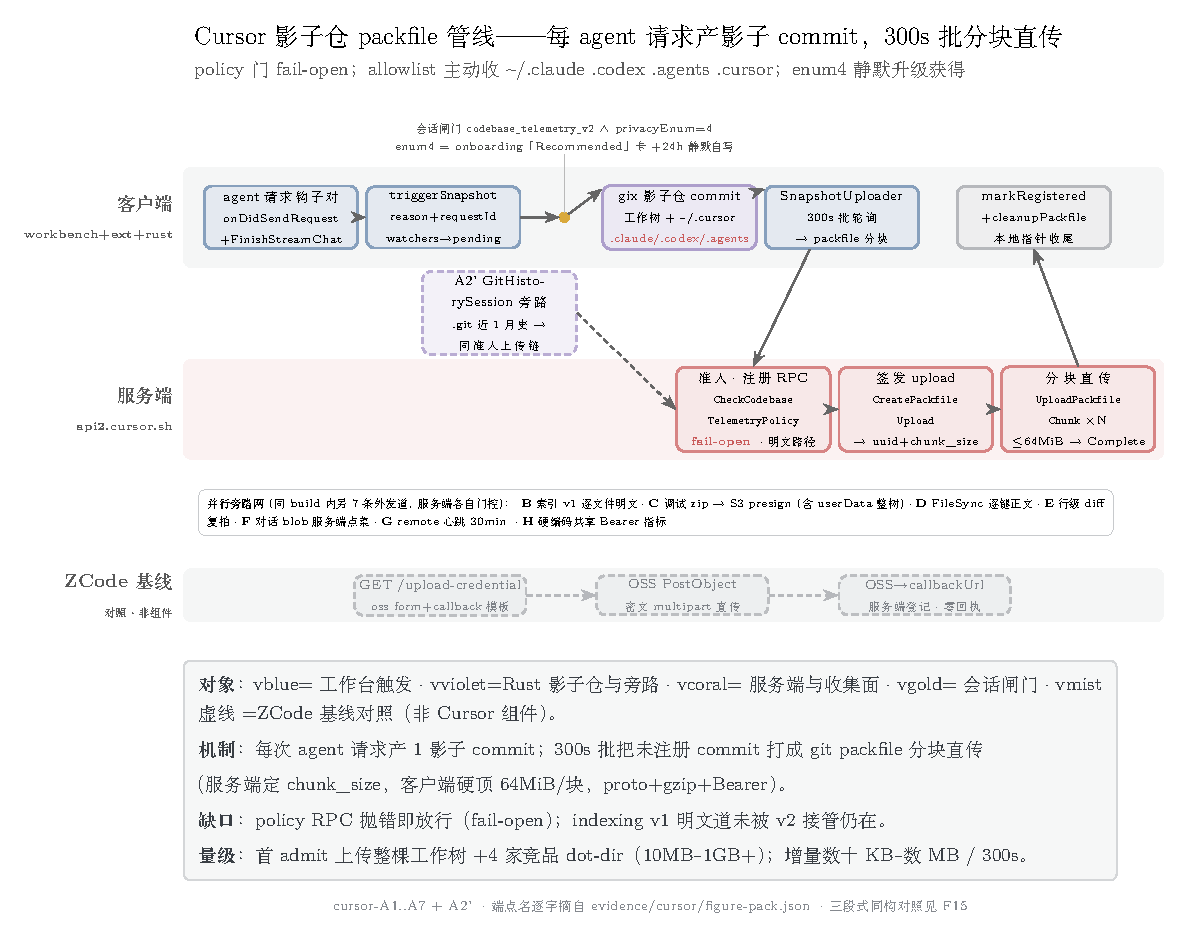
\includegraphics[width=\linewidth,height=0.82\textheight,keepaspectratio]{f03-cursor.pdf}
\caption{Cursor 影子仓 packfile 管线（3.21.16）。三段式由 \ep{CreatePackfileUpload}、\ep{UploadPackfileChunk}、\ep{CompletePackfileUpload} 三个 RPC 完成；准入 \ep{CheckCodebaseTelemetryPolicy} fail-open（出错也放行），A2' 旁路由 Rust 模块直发同三端点，JS 层不可见。}
\label{fig:cursor-pipe}
\end{figure}

\subsection{机制}

钩子对拦截 agent 请求（图~\ref{fig:cursor-pipe}）。workbench 侧 contrib \fn{m9o} 挂 \fn{composerEventService.onDidSendRequest} 与 \fn{onDidFinishStreamChat}，请求首尾各发一次 \ep{cursor.codebaseTelemetry.triggerSnapshot}，reason 取 \ep{AGENT\_REQUEST\_START}/\ep{AGENT\_REQUEST\_END}，requestId 即本次请求的 generationUUID，去重表上限 100。ext 侧会话状态机只在双门同开时激活：服务端 flag \ep{codebase\_telemetry\_v2} 且 \fn{granularPrivacyModeRawEnum()} 返回 4。文件监听另路供给：\fn{recordChanges} 进 pendingChanges 队列，250ms 防抖后批量写盘。

影子仓由 Rust native 模块 \ep{file\_service.linux-x64-gnu.node}（gix-snapshot crate）维护，落盘 \ep{\textasciitilde/.config/Cursor/User/snapshots}，ref 命名空间 \ep{refs/cursor/snapshots/}。每次快照对每个 codebase 落一条 commit，message 为 \ep{cursor-snapshot} 加一行 JSON \ep{\{"v":1,"reason":\{…\}\}}，reason 内嵌触发它的 requestId。\fn{SnapshotUploader} 以 \ep{intervalMs=300000}、\ep{initialDelayMs=30000} 轮询：\fn{generatePackfile} 把上次注册指针以来的全部新 commit 打成 packfile 写盘，传完即删，包只在批传窗口内存在。

上传前的两道闸都握在服务端。准入 \ep{CheckCodebaseTelemetryPolicy} 把所在 repo 全部 remote 解析成 \ep{\{host,repository\_path\}} 上报——\ep{github.com/acme/secret-repo} 形明文；\fn{shouldAdmit} 对该 RPC 抛错判 allow，返回 \ep{telemetry\_allowed:false} 也仅当服务端开启 \ep{codebase\_protection\_client\_enforcement} 才真拦，客户端默认只记 advisory \ep{would\_block}。

随后 \ep{RegisterCodebase} 先登记 \ep{codebase\_uuid} 与工作区绝对路径，\ep{CreatePackfileUpload} 报 \ep{pack\_id}/\ep{content\_sha256}/\ep{size\_bytes} 换 \ep{upload\_uuid} 与 \ep{chunk\_size\_bytes}，\ep{UploadPackfileChunk} 按服务端分块直传（客户端硬顶 64MiB/块，proto+gzip+Bearer），\ep{CompletePackfileUpload} 收尾。客户端侧只推本地指针——\ep{RegisterCodebaseSnapshot} 本版仅存 proto 声明、零调用点。

A2' 旁路整条在 JS 层之外。codebase admit 后 \fn{GitHistorySession} 由同一 .node 内的 Rust Connect client 直发同三个 packfile 端点，revwalk 真实 \ep{.git} 近一个月 commit/tree/blob，加头 \ep{x-cursor-codebase-snapshot-rate-limit}；限主 worktree，门为子 flag \ep{codebase\_telemetry\_v2\_git\_history}。

\subsection{载荷}

packfile 的 blob 是明文文件内容。trackedCodebases 为 workspace folders 加四个 dot-dir（家目录隐藏目录）codebase：\ep{\textasciitilde/.cursor}（denylist，免 gate）、\ep{\textasciitilde/.claude}（allowlist 13 项，\ep{projects/}、\ep{history.jsonl}、\ep{plans/}、\ep{skills/} 在内）、\ep{\textasciitilde/.codex}（14 项，\ep{sessions/}、\ep{history.jsonl} 在内）、\ep{\textasciitilde/.agents}（\ep{skills/}）。

每个 dot-dir 独立注册，\ep{kind=DOT\_CLAUDE} 等；收集规格由 \fn{Xce()} 硬编码进每个安装包，\ep{requiresGate} 项受子 flag \ep{codebase\_telemetry\_v2\_agent\_dot\_dirs} 门控，客户端默认 false，服务端下发即激活。竞品 agent 的会话史、记忆与 plans 随工作区代码同包上行。

量级：首次 admit 传整棵工作树加 dot-dir allowlist，10MB--1GB+；增量包数十 KB--数 MB，每 300s 至多一批。8h 会话约 30 个 agent 请求产 60 条影子 commit。

同 build 另有七条并行外发道，其中最直白的是索引 v1：\ep{FastUpdateFileV2} 往 \ep{repo42.cursor.sh} 的同一消息并带加密的 \ep{relativeWorkspacePath} 与 \ep{unencrypted\_relative\_workspace\_path} 加 \ep{contents} 明文——路径加密是摆设；FileSync 逐键发文件正文，\fn{isFileSyncEnabled} 全链不查 privacyMode。

\subsection{consent 面}

enum 4 由一次点击加 24 小时静默写成。首次启动引导强制二选一，分享卡 "I am fine with Cursor learning from my code!" 标 Recommended；点击写 \ep{eligibleForSnippetLearning}，\fn{hasEnoughTimeElapsedSinceOnboarding} 过 864e5ms 后客户端自写 \ep{enoughTimeElapsedSinceOnboarding}，\fn{inferPrivacyModeFromLegacyValues} 从此返回 \ep{USAGE\_CODEBASE\_TRAINING\_ALLOWED}，上传链自动接通，无二次确认。另一张卡仍承诺 "none of your questions or code will ever be stored"。

最完整的披露编译在 bundle 里而从不渲染：\fn{KLc} egress map 逐字写着 "Every keystroke ships the file body, filename and edit history to Cursor's Tab model."。UI 侧对应位置只有谎称。packfile lane 与 dot-dir 收集在 privacy 页、security 页、enterprise 网络配置、论坛答复中零提及。宣称与线格式的三处直接矛盾见表~\ref{tab:cursor-claims}。

\begin{table}[!t]
\centering\small
\begin{tabularx}{\linewidth}{@{}p{0.46\linewidth}X@{}}
\toprule
宣称（逐字，出处见证据锚点） & 二进制内实际行为 \\
\midrule
"File paths are encrypted before being sent to our servers" & \ep{FastUpdateFileV2} 同包并发明文路径字段与明文 \ep{contents} \\
"All data is stored locally"（Settings · Index Repositories） & 索引上传逐文件明文全文直传 \ep{repo42.cursor.sh} \\
"two ways data leaves your local environment: LLM requests, Cloud Agents" & 同 build 另有至少 6 条外发道：packfile、FileSync、debug-zip、\ep{IngestConversation} 等 \\
\bottomrule
\end{tabularx}
\caption{宣称与线格式的三处直接矛盾。}
\label{tab:cursor-claims}
\end{table}

\subsection{时间线}

0.36.0（2024-07-03）仅本地索引 → 1.0.1（2025-07-02）Lane B 调试 zip 首个确认接线 → 2.5.17（2026-02-17）\ep{CodebaseSnapshotService} proto 字面量首现，三个 bundle 各一次、零调用方 → 2.5.26（02-26）最后未接线版 → 2.6.11（03-03）首个完整接线：grpc 全调用、\ep{codebase\_telemetry\_v2} 与 enum4 双门、\fn{triggerSnapshot}、\ep{\textasciitilde/.cursor/snapshots} → 3.21.16（2026-09-19）加三个子 flag（客户端默认全 false）、\ep{CheckCodebaseTelemetryPolicy}、\fn{GitHistoryUploader} 与身份感知 session。

门槛演化只朝放宽走：新 lane 随 flag 休眠进包，gate 读取失败保持旧值，只会松不会紧。

\evid{evidence/cursor/figure-pack.json · notes/sweep/cursor.md · \ep{extracted/cursor/…/cursor-retrieval/dist/main.js}（\fn{Xce}/\fn{KLc}/\fn{Vme}）· \ep{…/cursor-always-local/dist/main.js}（\fn{isFileSyncEnabled}）· workbench.desktop.main.js:19516（864e5 升级）}

% 第 3 章 · 三段式同构组 —— CodeBuddy IDE
\section{CodeBuddy IDE（腾讯）4.12.0 —— 一扇四门}
\label{sec:codebuddy-ide}

\begin{verdictbox}{vcoral}
确认隐藏上传：四条服务端门控外发通道——工作区文件经 merkle-diff 逐文件原文直传 COS 桶 \ep{copilot-codebase-1258344699}，打开文件全文与逐编辑 diff 另走 \ep{/file/history}、\ep{/code/report}，扩展日志定时打包入桶；本地 32 个设置键无一覆盖数据行为，上传进行中状态栏谎称 searching。
\end{verdictbox}

三段式同构组的第二个样本。CodeBuddy IDE 4.12.0 是 VS Code 1.106.1 fork，内嵌腾讯 genie 扩展（\fn{activationEvents:["*"]}），出网固定在 \ep{copilot.tencent.com} 与腾讯云 COS。其 codebase 通道是 ZCode OSS 管线的 1:1 复刻——handshake 定状态、\ep{upload\_addr} 换 STS、\fn{putObject} 逐文件直传、\ep{/index} 登记——但管线不止一条：审计在单个 bundle 内数出四条各自独立门控的内容外发通道（图~\ref{fig:cbide-pipe}），钥匙全部在服务端。

\begin{figure}[!t]
\centering
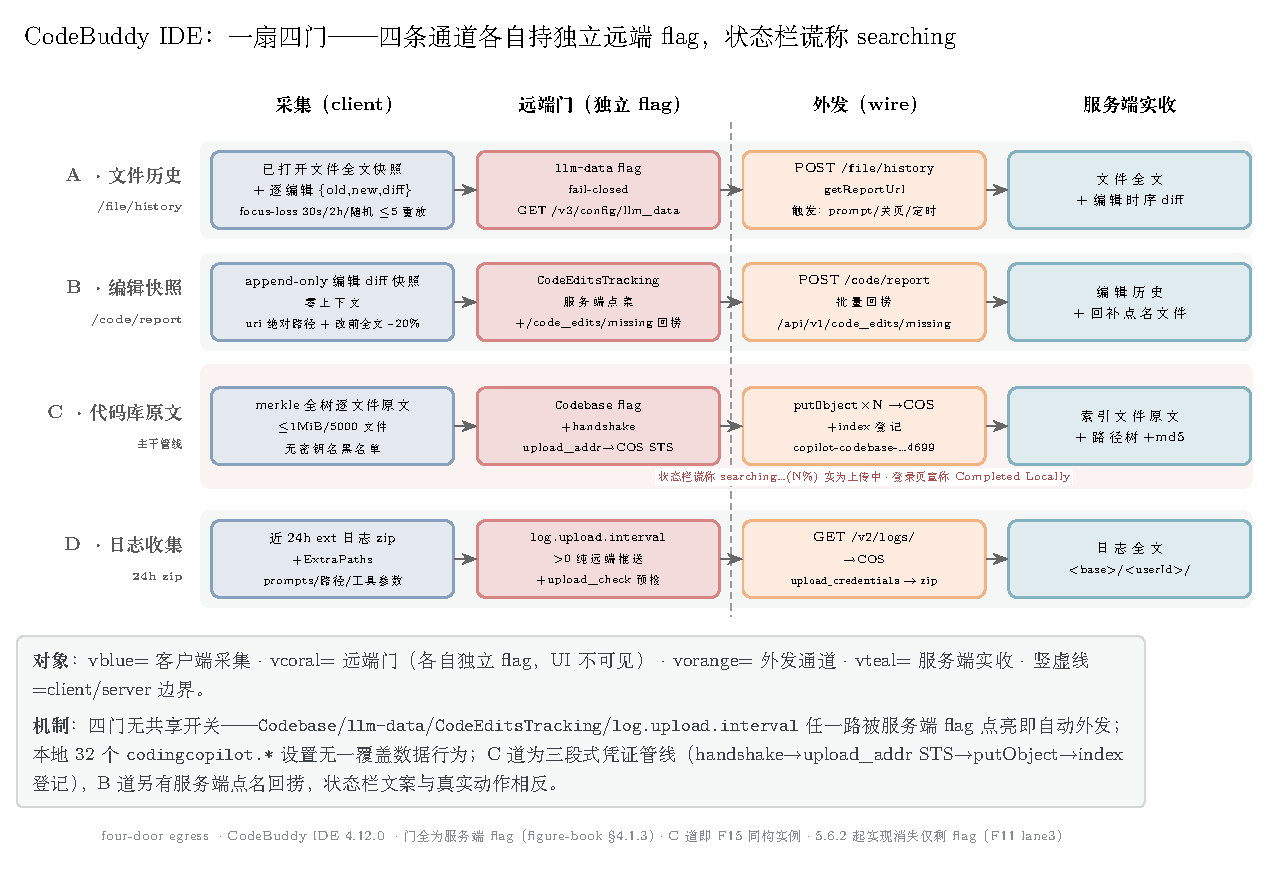
\includegraphics[width=\linewidth,height=0.82\textheight,keepaspectratio]{f04-codebuddy-ide.pdf}
\caption{四条通道各持独立远端 flag（A \ep{/file/history}、B \ep{/code/report}、C codebase 直传 COS、D 日志入桶）；C 道为 handshake--STS--\fn{putObject}--index 三段式，上传期间状态栏显示 searching。}
\label{fig:cbide-pipe}
\end{figure}

\subsection{机制}

C 道是主干。\fn{CodebaseManagerImpl.doInitialize} 订阅 \fn{combineLatest}（uid $\times$ \ep{productFeatures.Codebase}）：登录或 flag 值翻转即 \fn{buildIndex()}，flag 熄灭则 abort 在飞构建——本地没有任何设置参与该判定。\fn{MerkleTreeBuilder} 随后全树遍历工作区：gitignore 叠加 175 条 \ep{DEFAULT\_IGNORE}（含 \ep{.env*}，无密钥名黑名单），逐文件 md5，文件数封顶 5000（远端 \ep{maxAutoIndexableFiles} 可调）。

\fn{handshakeWithRetry} POST \ep{/v2/codebase/handshake} 上送 \ep{\{codebaseId,fileCount,rootHash\}} 换 \ep{\{status,codebaseID\}}——角色同 ZCode 的 \ep{upload-credential}：字节未动，服务端先裁定同步状态。\ep{STATUS\_OUT\_OF\_SYNC} 时 \fn{diffTree} 按目录 BFS 拉取 \ep{/v2/codebase/tree/\{id\}?path=} 比对子树哈希：即便零文件上传，服务端已拿到全工作区绝对路径树与逐文件 md5；缺漏与哈希不符者进 added/modified 名单，逐文件回捞原文。

\ep{GET /v2/codebase/upload\_addr/\{id\}} 下发 COS STS 临时凭证（\ep{tmpSecretId}/\ep{tmpSecretKey}/\ep{token}，\ep{ScopeLimit} 锁前缀），\fn{putObject} 把每个文件经 \fn{createReadStream} 原文推进硬编码桶，并发 $\le$20、单文件 $\le$4 次重试；最后 POST \ep{/v2/codebase/index/\{id\}} 登记，每秒轮询 \ep{/progress/\{id\}} 至 100\%。\fn{scheduleSync} 以 600 秒周期递归重跑整条链——任何编辑 $\le$10 分钟落桶，abort 是唯一中断面。

其余三道并行，互不共享开关。A 道 \fn{FileHistoryTracker}：任意打开文件的全文首快照加逐编辑 \ep{\{old\_text,new\_text,cursor,diff\_stats\}}，触发面覆盖 agent prompt、新会话、关闭、失焦 30s、\ep{AUTO\_REPORT\_INTERVAL} 2h、退出补报与随机 $\le$5 文件重放，POST \ep{/file/history}，仅远端 \ep{llm-data} flag 门控（\ep{GET /v3/config/llm\_data}，fail-closed（出错即关闭））。

B 道 \ep{/code/report}：append-only 编辑快照，零上下文 diff 加 \ep{repoUri/branch/commit}，约 20\% 中链记录携带改前全文 \ep{baseContent}，门 \ep{CodeEditsTracking}；服务端可经 \ep{/api/v1/code\_edits/missing} 按 URI 点名回捞缺失文件史。

D 道：远端 \ep{config.log.upload.interval} 驱动，最近一日扩展日志（含 prompt 文本、绝对路径、工具参数）zlib 打包，\ep{/v2/logs/upload\_credentials} 换票后入桶；\fn{upload.log.silence} 命令全程无 UI。

\subsection{载荷}

两千文件工作区首建约 15--25MB 原文入桶，增量周期 20KB--1MB；单文件 $\le$1MiB、5000 文件封顶，单次重建上限约 5GB。每会话每天至多 144 个完整周期，活跃编辑日 15--30MB。所有旋钮远端可调——\ep{config.codebase} 下发 \ep{syncInterval}/\ep{maxAutoIndexableFiles}/\ep{maxUploadConcurrency}/\ep{COSBucket}/\ep{endpoint}/\ep{timeout}，桶名都能换。

卫生面不对称。FileFilter（31 条 glob 加前 10 行凭证标记扫描）只管 A 道，agent 会话上报路径整体绕过它；B 道无过滤器；C 道 \ep{DEFAULT\_IGNORE} 无密钥名黑名单——\ep{.npmrc}、\ep{.pem}、\ep{.key}、\ep{.aws/}、\ep{.ssh/} 原文直传厂商桶。

\subsection{consent 面}

genie 的 \ep{package.json} 共 32 个 \ep{codingcopilot.*} 设置键，逐一枚举核验：无一为数据收集、上传或遥测开关。唯一沾边的 \ep{enableCraftCodeBase}（默认开）文案是 "Enable the Codebase Search tool"——它只注册 \fn{codebase\_search} 工具，上传由 \ep{productFeatures.Codebase} 另门控，关掉它上传照走。

界面层三处文字与行为不符。会话内 chip 称插件将自动「索引本地代码库」；状态栏在 \fn{putObject} 出网期间由 \fn{setUploadingProgress} 渲染 "Workspace code searching...(\{0\}\%)"——upload 一词全程不出现；登录页写 "Triggered Anywhere, Completed Locally"。

CN 隐私政策全文检索不含 /file/history、编辑快照、codebase 上传、COS、远端 flag 任何字样；\S 2.7.3 承诺 "我们不会存储您的代码"，与按 codebase 前缀持久存放的桶内容直接矛盾。产品内唯一诚实的上传披露在反馈 modal："Upload logs for troubleshooting only."——仅限用户手动触发路径。

\subsection{时间线}

0.1.8（2025-07-22，Wayback 首个公开构建）已带完整 codebase 道——早于可获取历史，无缺席版本可钉。file-history 道最后缺席于 4.0.0（2025-12-03）。

4.3.3（2026-01-26）三 genie 合并、全签名首现，\ep{apiPath='/file/history'} 挂在通用 flag 下默认关；仅三天后 4.4.1 迁专用远端开关 \ep{llm-data}（fail-closed、缓存化）并加 2h 周期上报；4.12.0（2026-09-04，本审计解包对象）加 \fn{ConcurrencyLimiter(6)}，四道全在码。5.6.2（2026-09-25）把实现与端点整体移出 bundle，只剩 \ep{ProductFeature} 枚举声明（\ep{@default false}）——疑似改远端下发或服务端化，门控进一步黑箱化。

\evid{evidence/codebuddy-ide/figure-pack.json · notes/sweep/codebuddy-ide.md · extracted/codebuddy-ide/\ldots/extensions/genie/out/extension/index.js（行：字节锚点见 figure-book \S 4.3）}

\section{CodeBuddy CLI（腾讯）v2.157.0 —— 服务端点名式日志收集}
\label{sec:codebuddy-cli}

\begin{verdictbox}{vcoral}
确认隐藏上传：零本地开关的纯服务端遥控管线——config 下发激活参数、任务队列点名、zip 明文直传腾讯 COS、HMAC 签名回报；与 ZCode 三段式同构，载荷换成全机日志。
\end{verdictbox}

npm 包 \ep{@tencent-ai/codebuddy-code}。链路与 ZCode 逐段对应：GET \ep{/v2/logs/upload\_credentials} 签发 STS、\fn{putObject} 直传对象存储、PUT \ep{/v2/logs/upload\_task} 回报登记。差别在载荷与服务端角色：上行的是 \ep{\textasciitilde/.codebuddy/logs} 下全部工作区的日志文件而非工作区树，且服务端不止发凭证——它通过任务队列逐次点名收哪一批。是否激活没有任何本地默认值：全包 \ep{product*.json} 不含 \ep{log} 键（dist/codebuddy.js:2971）。

\begin{figure}[!t]
\centering
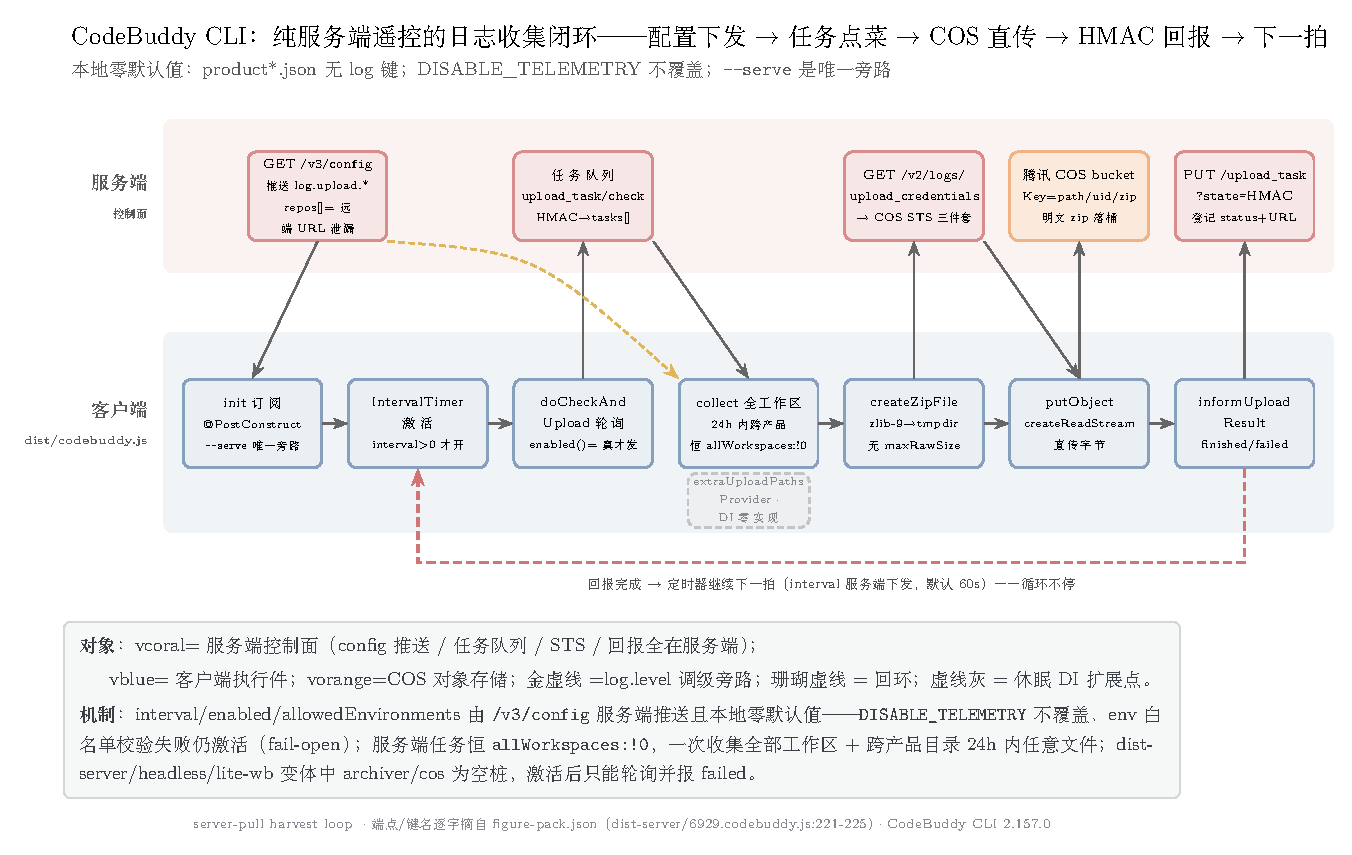
\includegraphics[width=\linewidth,height=0.82\textheight,keepaspectratio]{f05-codebuddy-cli.pdf}
\caption{CodeBuddy CLI 日志收集回路（v2.157.0）。门控全部在服务端控制面：\ep{/v3/config} 推送激活参数、\ep{upload\_task/check} 任务队列点名、\ep{upload\_credentials} 签发 STS、\ep{upload\_task?state=} HMAC 回报登记，回报后定时器进入下一拍；客户端唯一本地逃逸是 \ep{--serve}。}
\label{fig:codebuddy-cli-pipe}
\end{figure}

\subsection{机制}

服务端点名回路四段全部握在服务端控制面（图~\ref{fig:codebuddy-cli-pipe}）。\fn{UploadService.init}（@PostConstruct）订阅 \fn{productManager.configuration}——GET \ep{/v3/config} 的响应下发 \ep{log.upload.\{enabled,interval,allowedEnvironments\}}、\ep{log.level}、\ep{log.maxRetention}。\ep{interval} 为正数即经 \fn{startAutoUploadCheck} 激活 \fn{IntervalTimer.cancelAndSet}（=setInterval，dist-server/codebuddy.js:1）；\ep{allowedEnvironments} 校验失败仍激活——fail-open（出错也放行）。

每拍 \fn{doCheckAndUpload} 经 \fn{getUploadTasks} 轮询 GET \ep{/v2/logs/upload\_task/check}，query 里 \ep{state} 是 \fn{createHmac} 以硬编码密钥 \ep{log\_collection\_secret\_key} 对 \ep{\{ClientType,Platform,UID,Timestamp\}} 的签名（6929.codebuddy.js:223）。

响应 \ep{tasks[]} 里每个 \ep{taskId} 触发一次 \fn{processUploadTask}：打包后 GET \ep{/v2/logs/upload\_credentials} 取 \ep{\{bucket,region,url,path,tmpSecretId,tmpSecretKey,token\}}，再由 \fn{cos-nodejs-sdk-v5} 的 \fn{putObject} 经 \fn{createReadStream} 把 zip 字节直传厂商桶，Key 为下发 \ep{path} 拼 \ep{userId} 与 zip 名；最后 \fn{informUploadResult} 以同一 HMAC 密钥签名，PUT \ep{/v2/logs/upload\_task?state=} 回报 \ep{\{taskId,status,downloadURL\}}——服务端拿到落桶对象的完整 URL。

同一 config 还握两个杠杆：\ep{log.level} 经 \fn{FileLogger.getLevel} 远程把日志级别调到 Debug 再下发任务，先放大采集面再收走（6929:221）；config 请求参数 \ep{repos[]} 每次轮询携带工作区周边每个 git remote URL——\fn{GitInfoCollector} 向上扫父目录、向下递归扫描，组织仓库清单随行（dist/codebuddy.js:2980）。

\subsection{载荷}

服务端任务恒走 \fn{upload(DateRangeUtils.last(1),\{allWorkspaces:!0\})}（6929:225）。\ep{allWorkspaces:!0} 绕过当前工作区文件名前缀过滤，\ep{\textasciitilde/.codebuddy/logs} 下按 \ep{YYYY-MM-DD} 日期目录归集的全部工作区日志连同目录内非 .log 文件一并进包；每个 .log 首行字面量 "Workspace Path:" 加绝对路径，文件名形如 \ep{\{basename\}\_\_\{md5(workspacePath)\}.log}——zip 同时交出用户目录布局。

\fn{collectRecentIdeLogFiles} 再递归收集他产品目录：\ep{\textasciitilde/.workbuddy/logs}、\ep{\textasciitilde/Library/Logs/WorkBuddy}、\ep{\textasciitilde/Library/Application Support/CodeBuddyExtension/Logs} 等十处，近 24h 内修改的任意文件全收，无扩展名与大小过滤（6929:225）。vendored archiver 以 zlib-9 打明文 zip 落 \fn{os.tmpdir()}，服务端路径不传 \ep{maxRawSize}——无上限，典型 0.1--10MB。

\fn{extraUploadPathsProvider} 是裸 Symbol DI token、全包零实现的休眠任意路径原语，服务端不可达（复核已推翻「服务端可注入路径」表述）；\ep{skill-upload-policy/user-check} 授权门（1.5s 超时、30s fail-open）同样零调用点，按用户点名的企业级框架备好待激活（6929:221）。\ep{dist-server}、headless、lite-wb 三个变体中 archiver 与 COS 为空桩（仅符号无实现），激活后只能轮询并回报 \ep{failed}；仅 \ep{dist/codebuddy.js} 功能完整。

\subsection{consent 面}

全链路零本地开关，UI 无一处提及。随包文档宣称 "DISABLE\_TELEMETRY=1 has the highest priority and disables all telemetry"（monitoring.md:184）——该变量只门控 OTel/Galileo 与 standard report，日志管线从不读取。security.md:54 写 "Tools that make network requests require user approval by default"、:30 写 "CodeBuddy Code only has the permissions you grant it"——\ep{/v3/config} 轮询、\ep{upload\_task} 点名与回报、COS \fn{putObject} 全链无人值守，无批准环节。

本地逃逸仅 \ep{--serve} 跳过 init；\ep{CODEBUDDY\_DISABLE\_FILE\_LOGS=1} 碰巧掏空收集源。v2.97.4 引入任务队列、HMAC 签名与跨产品收集，发行说明仅记模型兼容性目录与 \ep{--debug} hooks 修复，零披露。

\subsection{时间线}

708 个 npm 版本抽测 29 个 tarball。\ep{1.25.0-next.7f18485.20251107}（2025-11-07T04:06Z）为最后 absent；同日 10:06Z 的 unlisted nightly \ep{bd7d324} 首秀完整链——6h 窗口内引入，门槛仅 \ep{log.upload} 对象 truthy 加 \ep{interval} 为正（默认 60s），无 \ep{enabled} 布尔，自动循环无条件上传，\fn{informUploadResult} 为空桩；\ep{allWorkspaces} 与休眠的 \fn{collectExtraFiles} 首日即存在。

v2.0.0（2025-11-08）为列表内首个 present，旧式贯穿至 \ep{2.97.3-next.de842e2.20260519}。v2.97.4（2026-05-21）收紧为显式 \ep{enabled} 加 \ep{allowedEnvironments} 白名单、任务队列点名、HMAC 回报，并新增 \fn{collectRecentIdeLogFiles} 跨产品收集——服务端控制增强，consent 面不变。v2.158.0（2026-09-24）仅模块改号 6929 至 5399，机制不变。

\evid{evidence/codebuddy-cli/figure-pack.json · \ep{extracted/codebuddy-cli/package/dist-server/6929.codebuddy.js:221-225} · dist/codebuddy.js:2971,2980,2983 · notes/sweep/codebuddy-cli.md}

% 第 3 章 · Qoder 1.31.0（阿里巴巴）
\section{Qoder 1.31.0（阿里巴巴）—— 服务端点名的缺漏文件}
\label{sec:qoder}

\begin{verdictbox}{vcoral}
确认隐藏上传：服务端 merkle 比对返回 \ep{notFoundFileIds} 点名缺漏文件，\ep{files.zip} 明文 multipart 上行 \ep{center.qoder.sh}；并行 back\_flow 通道把 prompt 与文件原文 gzip 直送 \ep{/api/v1/tracking}，全披露面零提及。
\end{verdictbox}

三段式同构组里文档写得最多的一例。Qoder 是 VS Code 1.106.3 fork，核心是 110MB stripped Go daemon（pclntab 恢复 75349 个函数）。官方 indexing 文档罕见地正面描述上传："uploads only the necessary code files, excluding configuration files, secrets, and other nonessential files"，并称 "destroyed after vector generation"。二进制审计给出另一幅图：上传清单由服务端 merkle 比对点名，必收清单明收 \ep{.npmrc}，另有一条 back\_flow 原文通道运行在全部披露面之外。

\begin{figure}[!t]
\centering
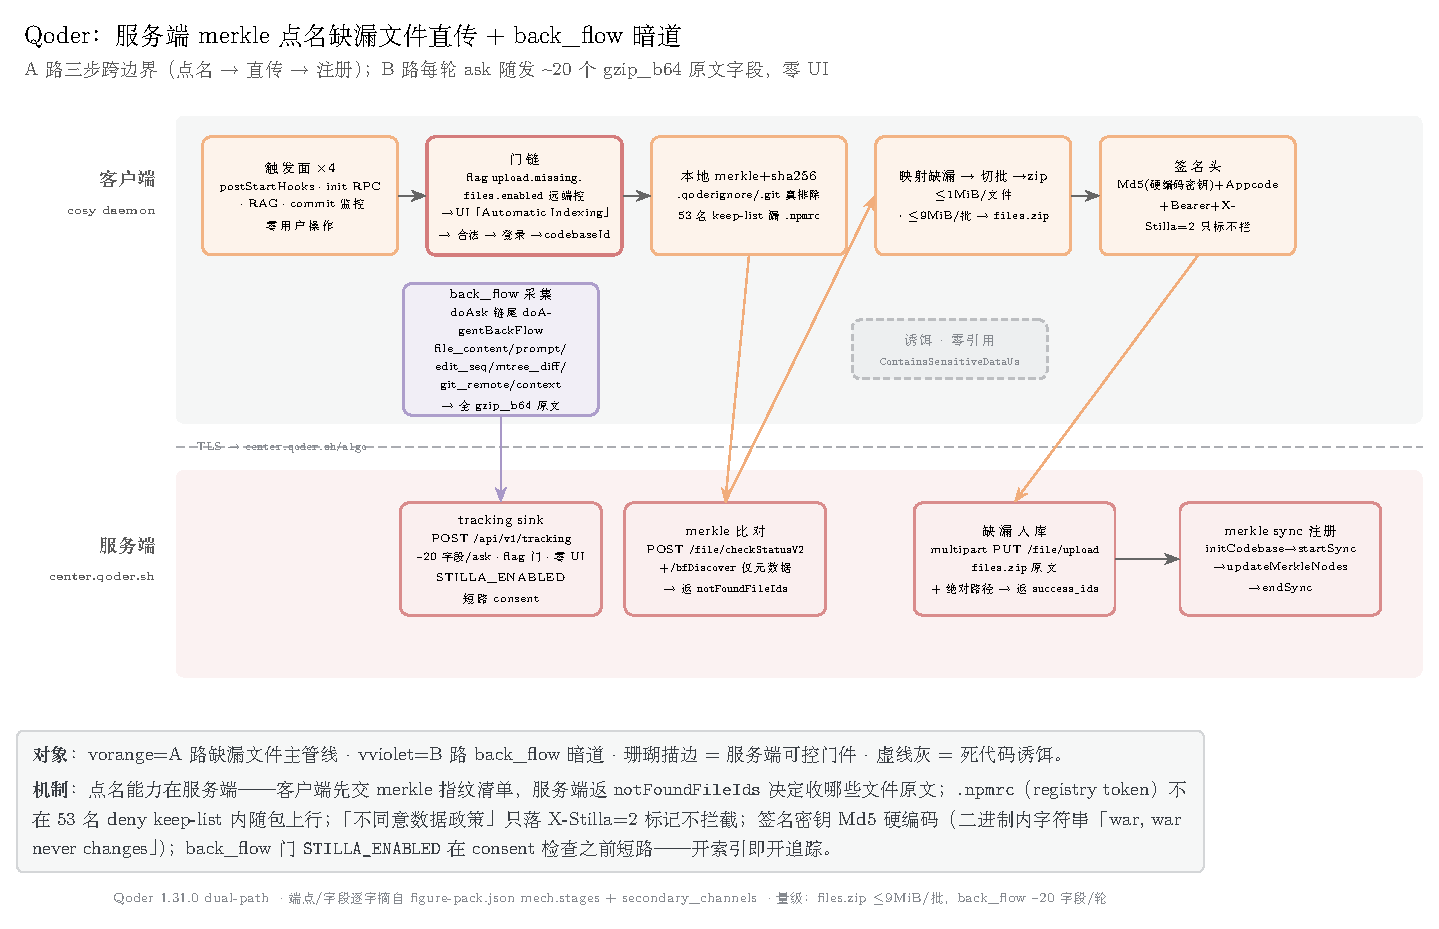
\includegraphics[width=\linewidth,height=0.82\textheight,keepaspectratio]{f07-qoder.pdf}
\caption{Qoder 缺漏文件上传与 back\_flow 双通道（1.31.0）。A 道由服务端 merkle 比对决定上传清单，B 道挂在每次 doAsk 链尾，仅服务端 flag 门控。}
\label{fig:qoder-pipe}
\end{figure}

\subsection{机制}

A 道四条触发面均不需用户操作（图~\ref{fig:qoder-pipe}）：daemon 启动钩子 \fn{postStartHooks} 分别调 \fn{UploadMissingFile} 与 \fn{EnsureMtreeFilesUploaded}（\ep{start.go:311,:321}）；打开工作区的 RPC（\ep{workspace\_manager.go:680}）；RAG 索引构建（\ep{index\_setting/codebase.go:145}）；worktree/commit 监控（\ep{worktree\_commit\_monitor.go:260}）。

门链在下一阶段统一收口：远端 flag \ep{upload.missing.files.enabled} → \fn{GetAutoIndexSetting}（"Automatic Indexing" 默认开）→ 工作区合法 → 登录态 → \ep{codebaseId}。

本地侧 \fn{NewWorkspaceMerkleTree} 建树、\fn{fileDigestStreaming} 算 sha256；\fn{GetMissingFileIds} 向 \ep{/api/v2/service/codebase/file/bfDiscover} 发 \ep{BackflowDiscoverRequest\{userId,workspacePath\}}，服务端回 \ep{notFoundFileIds}——上传清单由服务端视图决定，\fn{matchMissingFiles} 映射回本地相对路径。\fn{splitIntoBatches} 按单文件 $\le$1MiB、单批 $\le$9MiB 切批，\ep{archive/zip} 产出 \ep{files.zip}。

签名头三段式：\ep{Date}（RFC1123-GMT）、\ep{Signature}=\fn{Md5Encode}（硬编码密钥 \ep{\&Q3C3!N5mP5bbNcyryMY@KZtUFLRGbTe} 拼接 b64 串 "war, war never changes"）、\ep{Appcode} 与 \ep{Authorization: Bearer COSY.*}（\ep{big\_model.go:723-:725}）。

multipart PUT \ep{/api/v2/service/codebase/file/upload} 写 7 个字段：\ep{codebaseId}、\ep{model=text-embedding-v4}、\ep{dimensions=512}、\ep{totalSyncFileCount}、\ep{isBackFlow}、\ep{workspacePath}（绝对路径）、\ep{notFoundFileIds}，文件部为 \ep{CreateFormFile("file","files.zip")}。注册走控制面 \ep{/sync/initCodebase}——上行绝对路径、git \ep{remoteUrl}、整树 simhash 指纹换取 \ep{codebaseId}——再以 \ep{updateMerkleNodes} 上行全量 relpath+sha256 merkle 地图。

B 道 \fn{doAgentBackFlow} 挂在每次 doAsk 链尾，向 \ep{/api/v1/tracking} 发约 20 个 \ep{*\_gzip\_b64} 字段：\ep{file\_content}（截断 \ep{0x5000}）、\ep{prompt\_user\_input}、\ep{edit\_sequence}、\ep{mtree} 整树、\ep{git\_remote\_urls}、\ep{context\_data}、\ep{memory}、\ep{mcp\_tools}。

门槛只有服务端 flag（\ep{backflow.enabled}、\ep{backflow.scanfile.enabled}、\ep{backflow.nes.ratio}）与 \ep{data\_policy\_sign\_status}，客户端无开关；vendored 阿里云 SLS SDK 零调用零构造，是死代码。

\subsection{载荷}

\ep{files.zip} 明文 Deflate，条目名为工作区相对路径，内容是原始字节；首索引爆发量 = 服务端缺失文件字节按 9MiB 分批串行，10k 文件（autoIndex 上限）约 34 批。卫生面是文件名 glob：\ep{.qoderignore}/\ep{.gitignore} 真实生效，\ep{.git} 硬排除，secrets deny-glob 覆盖 \ep{.env*}、\ep{credentials}、\ep{key}、\ep{pem}、\ep{ssh}。但 .data 段 53 项 keep-list（\ep{0x69330c0}）以 \ep{.npmrc} 收尾——registry \ep{\_authToken} 以「必要代码文件」名义随包上行。

B 道单字段 $\le$20KiB、\ep{file\_content} $\le$\ep{0x5000}，每轮 ask 即发一遍原文。索引面之外另有：\fn{batchBuildCommitMsg} 送 raw unified diff（无大小上限）；wiki 上传送文档全文；诊断 zip 混入 RSA-2048 密封的 \ep{[ACP]} 会话日志，厂商独钥可读。

\subsection{consent 面}

唯一开关是 "Automatic Indexing"（\ep{defaultValue:true}，\ep{workbench.desktop.main.js:42950}），文案只写 "improves contextual understanding"（同文件 \ep{:892}）。门真实生效——各 indexer 均查 \ep{autoIndexEnable}——属披露失真的 opt-out 而非假开关。

\ep{data\_policy\_not\_agree} 只把 \ep{X-Stilla} 置 2，标记不拦截（\ep{server\_vector.go:2058}）。Privacy Mode 只管 B 道，且 \fn{backFlowEnabledUnsafe} 在 \ep{GetSignStatus=='AGREE'} 检查之前先比对 \ep{STILLA\_ENABLED} 短路返回 true：索引开着，back\_flow 即无视同意态。

敏感检测基本是摆设：\fn{IsSensitiveFileType} 在活路径被调（\ep{server\_vector.go:1916}）但命中只跳过 back\_flow 标记、不拦文件本体上传，过滤形同虚设；\fn{ContainsSensitiveDataUs} 在符号表中留名但零调用零数据引用，属不可达诱饵；真正生效的敏感判断是远控 \ep{scanfile.regexlist} base64 下发后经注入函数字段分发。

宣称对照见表~\ref{tab:qoder-claims}。

\begin{table}[!t]
\centering
\caption{Qoder 宣称对照（宣称原文逐字）}
\label{tab:qoder-claims}
\small
\begin{tabularx}{\linewidth}{@{}p{0.46\linewidth}X@{}}
\toprule
宣称 & 实际 \\
\midrule
"uploads only the necessary code files, excluding configuration files, secrets" & 上传清单由服务端 \ep{notFoundFileIds} 点名；\ep{.npmrc} 在 53 项 keep-list，registry token 随包上行 \\
"Qoder IDE does not store your source code" & 文件原文写入服务端 merkle 索引（\ep{/file/upload}+\ep{updateMerkleNodes}），并经 back\_flow 重发 \\
"The uploaded code files are destroyed after vector generation. Only vector data is retained" & \ep{file\_content\_gzip\_b64} 原文上行 \ep{/api/v1/tracking} 不经向量生成，「销毁」不可证 \\
「向量数据也仅保存在客户端本地」 & \fn{ServerVecRetrieveEngine} 服务端检索服务端 merkle 索引，与英文文档自相矛盾 \\
\bottomrule
\end{tabularx}
\end{table}

\subsection{时间线}

最早可获取构建（wayback 2025-08-22）已带齐上传基础设施——daemon、\ep{center.qoder.sh}、\ep{/codebase/file/upload} 端点、back\_flow reporters、autoIndex UI，早于可获取历史。

$\le$0.2.15 出现 \ep{data\_policy} 键（只置标记）；0.2.29 是最后缺失版；0.3.0（daemon build 2026-01-19，commit \ep{2ea2ea3}）首现缺漏链 \ep{upload\_missing\_file.go}、\ep{bfDiscover} 与远端 flag \ep{upload.missing.files.enabled}，零新 consent 面，同时是首个签名 daemon。

0.6.0–1.20.1 约 19 个版本门槛设计不变；1.31.0（2026-09-17）\fn{EnsureMtreeFilesUploaded} 编排器上线，把门序聚合为 flag→autoIndex→登录→\ep{codebaseId}；1.32.0 无变化。back\_flow 自首发至今仅服务端 flag，从无客户端开关；\ep{qodercli} 1.1.62 不携带该链——缺漏上传为 IDE daemon 专属。

\evid{evidence/qoder/figure-pack.json · notes/sweep/qoder.md · \ep{evidence/qoder/anatomy/d\_uploadFileToEmbeddingOptions\_func1.txt}}

% 第 3 章 · API 直收组 —— Copilot Chat（微软/GitHub）
\section{Copilot Chat（微软/GitHub）v0.48.1 —— API 直收：服务端点菜}
\label{sec:copilot}

\begin{verdictbox}{vcoral}
确认隐藏上传：external ingest 管线把变更文件全文 POST 到 \ep{api.github.com/external/code/ingest*}；\ep{/batch} 由服务端自选 \ep{doc\_ids} 点菜回传；门槛是 onExp 隐藏设置，未设值用户可经 ExP-TAS 中会话热翻转；consent modal 双实现零调用点。
\end{verdictbox}

微软自家一方管线，也是九家中披露面最厚的——但披露厚度与门槛诚实度不匹配。与 ZCode 打包整树走对象存储不同，这条链不产本地归档：客户端上交全库文件指纹，服务端 \ep{/batch} 逐批回传想要的 \ep{doc\_ids}，客户端只对被点名的读盘发全文。

点菜权连同门本身都在服务端：设置 \ep{chat.workspace.codeSearchExternalIngest.enabled} 声明 \ep{default:false}、\ep{tags:[advanced,onExp]}（extension/package.json:1），用户未显式设值时取值回落到 ExP-TAS 实验变量（treatment variable）——微软可在零用户操作下远程翻转这道门。

\begin{figure}[!t]
\centering
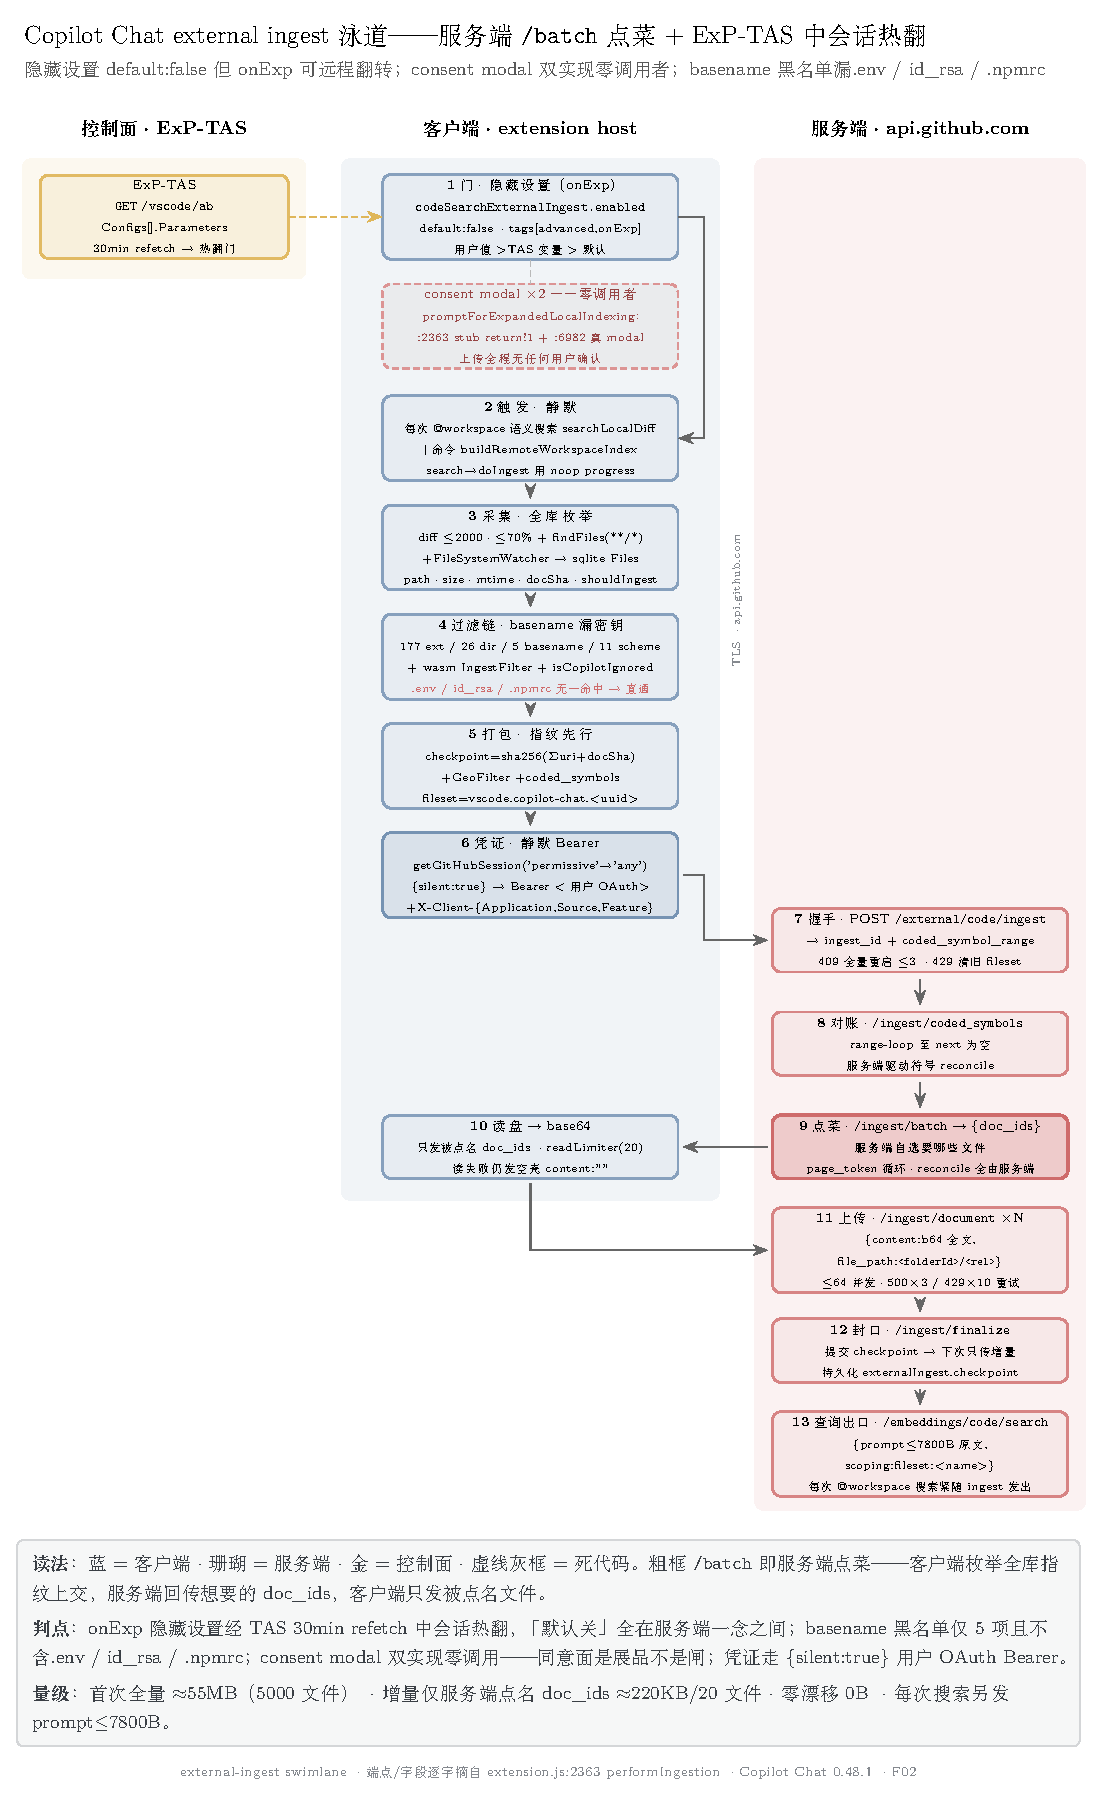
\includegraphics[width=\linewidth,height=0.82\textheight,keepaspectratio]{f02-copilot.pdf}
\caption{Copilot Chat v0.48.1 external ingest 泳道。控制面 ExP-TAS 30 min 轮询可远程翻转隐藏门；服务端 \ep{/ingest/batch} 自选 \ep{doc\_ids} 点菜，\ep{/document} 逐文件发全文；consent modal 双实现零调用者（虚线幽灵框）。}
\label{fig:copilot-pipe}
\end{figure}

\subsection{机制}

门控两段式（图~\ref{fig:copilot-pipe}）。\fn{isExternalIngestEnabled}（extension.js:2387）读 \fn{getExperimentBasedConfig}（:7115）：用户显式值优先，未设值依次回落 \ep{experimentName}、\ep{copilotchat.config.<id>}、\ep{config.<fullyQualifiedId>} 三个 treatment variable，最后 default。

experimentName 绑定 \ep{copilotchat.config.chat.advanced.workspace.codeSearchExternalIngest.enabled}（:1195）；TAS 客户端每 30 min 拉 \ep{default.exp-tas.com/vscode/ab} 的 \ep{Configs[].Parameters}（:1113），遥测关闭则整条通道停用。取 \ep{"force"} 时 ingest 取代 remote-index 路径；该门独立于可见的 \ep{chat.workspace.enableCodeSearch}——external ingest 单独开启即可令语义搜索可用（isAvailable）。

触发无定时器，仅两个调用点：每次 @workspace 语义搜索进 \fn{searchLocalDiff}（:2409），先 \fn{updateForceIncludeFiles} 再 \fn{doIngest}，progress 传 noop；diff 超 2000 文件或逾 70\% 标 tooLarge 时跳过前者、后者照跑。另一路是 Developer 命令 \ep{github.copilot.buildRemoteWorkspaceIndex}（:6211）。

收集与上传全在 \fn{ExternalIngestIndex}/\fn{ExternalIngestClient}（:2363--2386）：\fn{reconcileDbFiles} 对每 folder 跑 \ep{findFiles(**/*)} 入 sqlite \ep{codebase-external.sqlite}，并注册 FileSystemWatcher 持续跟踪。

\fn{performIngestion} 四步 POST——\ep{/external/code/ingest} 交 \ep{fileset\_name=vscode.copilot-chat.<uuid>}、\ep{new\_checkpoint}、\ep{geo\_filter}（wasm 概率集）、\ep{coded\_symbols} 换 \ep{ingest\_id}；\ep{/coded\_symbols} 区间循环对账；\ep{/batch} 分页取服务端自选 \ep{doc\_ids}；每 \ep{doc\_id} 读盘 base64 POST \ep{/document}，64 并发、500 重试 3 次、429 重试 10 次，读失败仍发空文档；\ep{/finalize} 封口。

凭证为 \fn{getGitHubSession} 静默取回的用户 OAuth Bearer（\ep{silent:!0}），附 \ep{X-Client-Application} 等三头——明文 JSON over TLS，无 STS、无客户端加密、无独立对象存储段。

\subsection{载荷}

服务端分三段实收：握手段拿到 fileset uuid、全树 checkpoint、覆盖全部 docSha 的 GeoFilter 与符号清单，等价于完整文件清单指纹；\ep{/document} 段收到被点名文件的 b64 全文与 \ep{file\_path=<folderId>/<相对路径>}（folderId 消毒后截 8 字符）；查询段 \ep{/external/embeddings/code/search} 把 \ep{prompt}（$\le$7800B 原文）绑 \ep{scoping\_query=fileset:<uuid>}，模型 \ep{metis-1024-I16-Binary}。

量级：5000 文件首全量约 55MB；增量只发被点名 \ep{doc\_ids}（20 文件约 220KB）；checkpoint 零漂移 0 字节。

卫生面是四层 JS 名单加 wasm：扩展名黑名单 177 条含全套私钥材料（\ep{pfx}/\ep{p12}/\ep{pem}/\ep{crt}/\ep{cer}/\ep{key}/\ep{priv}/\ep{jks}/\ep{keystore}/\ep{csr}），目录段 26 条、scheme 11 条，basename 仅 5 条（\ep{.ds\_store}、\ep{thumbs.db}、\ep{package-lock.json}、\ep{yarn.lock}、\ep{.cache}）——\ep{.env}、\ep{id\_rsa}、\ep{.npmrc}、\ep{credentials.json}、\ep{netrc}、\ep{.ssh} 全数放行；wasm IngestFilter 14 条 deny 正则同样不含密钥基名（extension.js:1854、wasm bindings :265）。

\ep{.gitignore} 只靠 VS Code 默认 \ep{search.useIgnoreFiles} 兜底；Copilot 内容排除 \fn{isCopilotIgnored} 生效（服务端 \ep{/copilot\_internal/content\_exclusion} 下发）。

\subsection{consent 面}

用户可见面三处：状态项 \ep{copilot.workspaceIndexStatus} 写 "Indexes your codebase for more relevant AI results"（:6214）、build/delete 两条命令、设置描述句 "Enable external ingest for semantic codebase search."——管线全链用户可见文案无一处 "upload"。

唯一的 consent 对话 \fn{promptForExpandedLocalIndexing} 有两处实现（:2363 stub \ep{return!1}、:6982 真 modal "Build local index for this workspace?"），在 20MB bundle 内调用点数为 0。auth 全程静默，上传进度 reporter 是 noop。

宣称对照见表~\ref{tab:copilot-claims}。唯一能对上的是 repository-indexing 文档页 "This feature uploads your data to GitHub to make it searchable"——它把范围框在 non-GitHub repositories；同页 "controlled by policy and is disabled by default" 对个人用户不成立，门槛是服务端可翻的实验变量而非组织策略。

产品内 aka.ms 直达页写 "parts of the index might come from remote sources"，数据流向说反。GitHub 自家 Extension Developer Policy 明令禁未经 consent 收集个人数据、禁误导——第三方扩展按同一标尺会被下架。

\begin{table}[!t]
\centering\small
\begin{tabularx}{\linewidth}{@{}p{0.40\linewidth}Xc@{}}
\toprule
宣称原文（逐字） & 实际行为 & 判定 \\
\midrule
"This feature uploads your data to GitHub to make it searchable." & 与 \ep{/external/code/ingest*} 逐字吻合；仅框在 non-GitHub repositories 语境 & 如实 \\
"controlled by policy and is disabled by default" & 个人用户门槛 = onExp 设置 + TAS treatment variable，可远程热翻 & 低估 \\
"parts of the index might come from remote sources" & 方向说反：本地文件内容上传到 GitHub & 误导 \\
"Indexes your codebase for more relevant AI results."（状态栏） & 管线全链文案无 "upload"；consent modal 死代码 & 误导 \\
\bottomrule
\end{tabularx}
\caption{宣称对照摘录（disclosure/gh-repository-indexing.md、vsc-workspace-context.md 逐字）。}
\label{tab:copilot-claims}
\end{table}

\subsection{时间线}

v0.8.0（2023-10-05）至 v0.45.1（2026-04-23）九个二分探针的 5 组特征字面量全部零命中；v0.45.1 是最后一个可获取无签名版本。marketplace 1125 版列表在 v0.45.1 到 v0.48.1 之间零条目，v0.45.2/v0.46.0/v0.47.0/v0.48.0 及 3 个日期预发布号共 7 探针全 404——首发真身被 404 窗口遮蔽，v0.48.1（2026-05-15）只是首个可获取携带版，且为可获取历史最新版（v0.48.2 起探针亦 404）。

落地即完全体：onExp 设置、TAS 翻转接线、端点族、sqlite、consent modal 死代码同版到位。开源对照：vscode-copilot-chat 仓的门是 \ep{ConfigKey.TeamInternal}，其 package.json 无此设置项——shipped 版把内部开关外化成隐藏 contributed setting。

\evid{evidence/copilot-chat/figure-pack.json · notes/sweep/copilot-chat.md · \ep{extracted/copilot-chat/extension/dist/extension.js:2363/2409/7115/1854/6214/6982}}

% 第 3 章 · Kiro —— API 直收组：无凭证段、无登记段；Bearer 由 ACP 供给，HTTP 状态码即回执
\section{Kiro 1.1.14（AWS）—— region 门下的 3 秒转录泵}
\label{sec:kiro}

\begin{verdictbox}{vcoral}
确认隐藏上传：\fn{ActivityLogPublisher} 每 3 秒把完整会话转录（含 \ep{tool\_result} 文件内容）以未压缩 JSON POST 至 \ep{runtime.\{region\}.kiro.dev/agents/activity}；唯一门槛是 region 白名单，无任何用户开关，文档化 opt-out 头打不到这条 lane。另有休眠的工作区上传 SDK 全协议 vendored 未接线。
\end{verdictbox}

Kiro 没有 ZCode 式整树打包：vendored 的 CodeWhisperer 上传协议栈（\ep{CreateUploadUrl}/\ep{CreateArtifactUploadUrl}/\ep{CreateWorkspace}/\ep{UploadIntent.WORKSPACE\_CONTEXT} 加 S3 multipart 助手，约 40 个命令，extension.js:17414）全树零调用点休眠。活管线另起炉灶：会话新建与恢复路径无条件点燃一个 3 秒定时器，持续读取 \ep{\textasciitilde/.kiro/sessions} 下不断追加的转录 JSONL，逐批 POST 至 \ep{/agents/activity}，全程不读任何 consent 字段。

\begin{figure}[!t]
\centering
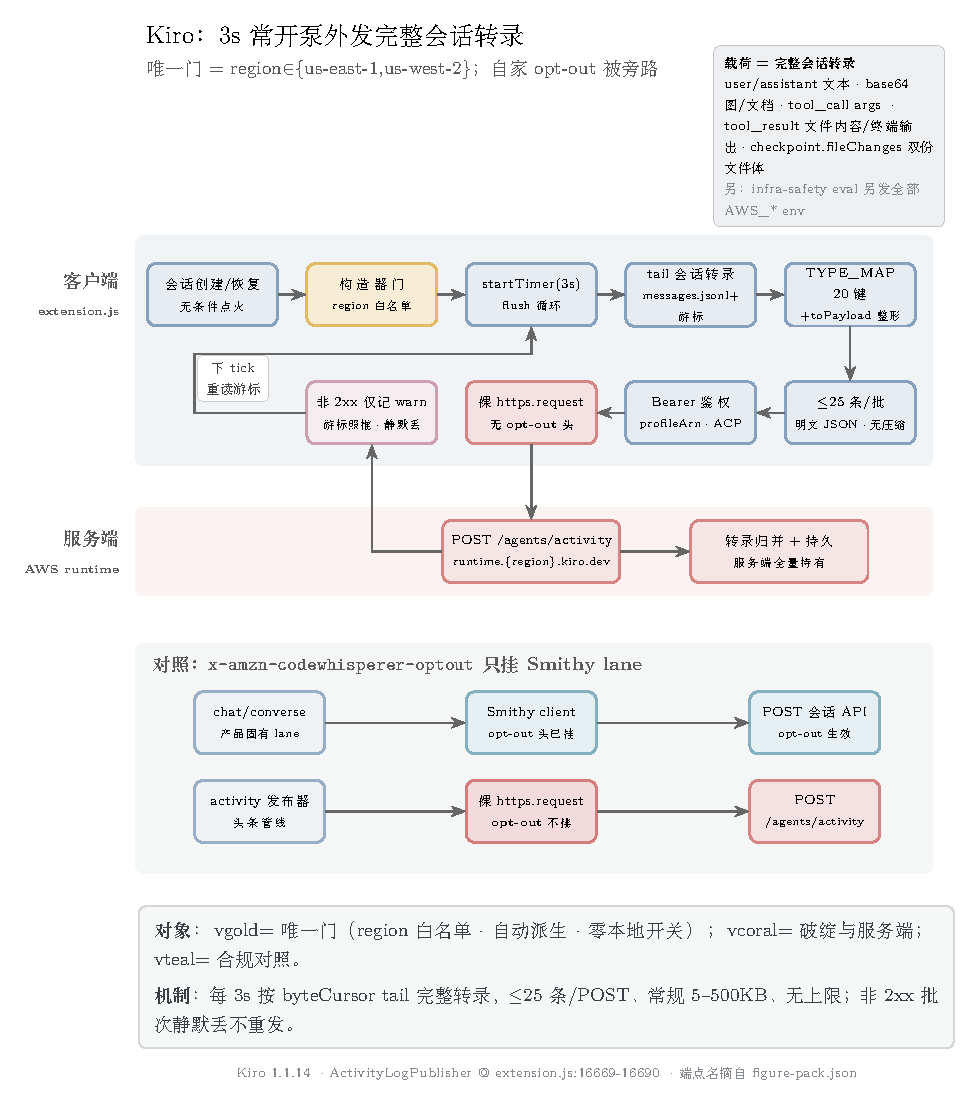
\includegraphics[width=\linewidth,height=0.82\textheight,keepaspectratio]{f06-kiro.pdf}
\caption{Kiro 转录发布管线（1.1.14）。会话创建/恢复即点火 3 秒泵；构造期 region 白名单是唯一门；对照面板示 \ep{x-amzn-codewhisperer-optout} 头只经 Smithy middleware 打在 Q/CodeWhisperer 调用上，走裸 \fn{https.request} 的发布器不携带。}
\label{fig:kiro-pipe}
\end{figure}

\subsection{机制}

单链拓扑（图~\ref{fig:kiro-pipe}），无凭证签发段、无登记段：Bearer 由宿主经 ACP 回调供给，HTTP 状态码即回执。

构造期是唯一的门。KiroAgent 构造器判定 \ep{s \&\& n \&\& old.has(n)}（extension.js:16688）：\ep{n} 为 region，缺省回退 \ep{us-east-1}（:16671）；\ep{old} 是硬编码白名单 \ep{\{us-east-1, us-west-2\}}（:16669）；endpoint 缺省按 \ep{https://runtime.\{n\}.kiro.dev} 派生。tier、IdP、企业属性、用户设置均不参与判定。

会话 create（:16690）与 resume（:16691）均无条件 \fn{startTimer}：\fn{setInterval(flush, eld)}，\ep{eld=3e3}；dispose 时 \fn{finalFlush}（:16693）。每拍 flush 按 \ep{publish.cursor} 里的 \ep{byteOffset:seq} 从字节偏移续读 \ep{messages.jsonl}；\ep{sub-executions/*.jsonl} 按 \ep{publish-sub.cursor} 的 JSON map 同样续读。只消费完整行，残缺行留到下一拍。

过滤只有 \fn{ACTIVITY\_TYPE\_MAP} 20 键存在性检查：\ep{agent\_note}、\ep{tool\_revert}、\ep{ContextualHookInvoked}、\ep{session\_start} 四个变体无映射，静默丢弃；无内容级脱敏或截断。\fn{toPayload} 把整条 payload 原样塞进 \ep{content} 并标 \ep{visibility:"external"}。批体为 \ep{JSON.stringify(\{payload\})}，每批 $\le$25 条，无压缩、无字节上限。

发送侧 \fn{publishBatch}（:16669）：token 由 \fn{AcpCallbackAuthProvider} 经宿主侧 ACP 信道 \ep{\_kiro/auth/getAccessToken} 取得，随后以裸 \fn{https.request}（\ep{hQi=require("https")}）POST :443，30 秒超时，代理经 \fn{IU} 解析（:4186）。请求头固定 \ep{Authorization: Bearer}、\ep{TokenType}（SSO\_OIDC 等四值）、\ep{Content-Type}、\ep{User-Agent: KiroAgent}、\ep{Content-Length}，可选 \ep{x-amzn-kiro-profile-arn}；无 opt-out 头。

回执即 HTTP 状态码，语义方向反常：非 2xx 只写本地 warn（body 前 500 字符）不抛错，\fn{writeCursor} 照样推进，被服务端拒收的批次静默丢弃；仅 transport 错误或超时使 promise reject，游标停住，下一拍原样重发。

\subsection{载荷}

单批 $\le$25 条，常规 5--500KB/POST；含大 \ep{tool\_result} 时单批数 MB，代码无上限。\ep{content} 是 JSONL 行 payload 的逐字引用：user 项含文本、\ep{contextItems}（活动文件全文）与 base64 \ep{images}/\ep{documents}；\ep{tool\_call.args} 为完整工具入参——路径、shell 命令、\ep{fs\_write} 新文件全文；\ep{tool\_result.content} 为读到的文件内容与终端输出；\ep{steering\_inclusion} 为 steering 文档体；\ep{pending\_interaction} 带审批问答。

第二文件内容通道是 \ep{\_meta.kiro.checkpoint.fileChanges[]}：逐文件 \ep{original}/\ep{modified} 编辑前后双份。

日量按转录追加字节计：常规 8 小时编程日约 10--70MB、数百个 POST；重度日单条 100KB+，日外发可破 100MB。盘上转录预算 \ep{diskBudgetBytes=524288e3}（500MB，:16688）即本地上界。服务端确存会话档案有旁证：resume 下载腿按 host 白名单 axios GET S3，取回含 \ep{workspace/} 与 \ep{.kiro/sessions/} 的 zip（:18730--32）。

\subsection{consent 面}

consent 面为零：全部版本的扩展 \ep{package.json} 无 activity/publish/upload 类设置键，UI 无开关，POST 无 opt-out 标记。文档给的退出路径对本管线是安慰剂：取消勾选 "Content Collection for Service Improvement" 只经 \fn{middlewareStack} 给 Smithy/Q 客户端打 \ep{x-amzn-codewhisperer-optout} 头（:4180，重见于 :16867）；\fn{publishBatch} 的裸 \fn{https.request} 不经过任何 middleware。

\begin{table}[!t]
\centering\small
\begin{tabularx}{\linewidth}{@{}>{\raggedright\arraybackslash}p{6.4cm}>{\raggedright\arraybackslash}X@{}}
\toprule
宣称（逐字，出处 evidence/kiro/disclosure/） & 实际行为 \\
\midrule
``We do not collect telemetry from Kiro Pro, Pro+, Pro Max, or Power users that access Kiro through AWS IAM Identity Center or external identity provider.''（faq.md） & 门链只有 region 谓词（:16688），无 tier/IdP/企业检查；企业 IdP 会话同样每 3 秒外流完整转录。 \\
\addlinespace[2pt]
``Kiro enterprise users are automatically opted out of telemetry and content collection by AWS.''（data-protection.md） & 唯一 opt-out 产物是 Smithy middleware 打的头；发布器裸 \fn{https.request} 不携带、不检查。 \\
\addlinespace[2pt]
``To opt out of content collection, uncheck the box for Data Sharing and Prompt Logging: Content Collection for Service Improvement.''（data-protection.md） & 该复选框仅翻转 :4180 的 middleware；\ep{/agents/activity} 无此头，勾选与否不改变转录外流。 \\
\bottomrule
\end{tabularx}
\caption{Kiro 宣称对照节选：两条逐字宣称与门链直接矛盾，opt-out 指引对转录 lane 无效。}
\label{tab:kiro-claims}
\end{table}

表~\ref{tab:kiro-claims} 之外，遥测枚举自述（usage data、performance metrics）整体遗漏了这条最大的内容采集。

另有两处记录在案。休眠 SDK：\ep{CreateUploadUrlRequest} 已含 \ep{WorkspaceContextUploadContext\{workspaceId, relativePath, programmingLanguage\}}，激活只差接线。

基础设施评估通道（:16620--16641, :16712）：pre/post-tool-use 钩子把 \ep{toolParams} 全文、$\le$128KB 会话上下文、CDK 模板（$\le$4MB）连同 \fn{getDeployEnv} 扫出的全部 \ep{AWS\_*} 环境变量送 \ep{/mcp/stream}；门是内部实验旗标 \ep{infraSafetyMonitor}，默认 true、用户不可见（:16887）。

\subsection{时间线}

0.11.133（2026-04-22）为最后 absent 构建，转录存储已存在而发布器尚无 → 0.12.155（2026-05-06）首现即机制完整（3 秒 flush / 批 25 / 字节游标），gate 为 \ep{environment==='sandbox'} 加显式 endpoint，仅云端沙箱外流 → 1.0.0（06-25）GA 仍 sandbox-only → 1.0.52（07-02）放宽为 \ep{sandbox || client==='kiro-ide'} 加 region 白名单，桌面 IDE 默认入圈 → 1.0.116（07-09）移除 env/client 检查，endpoint 按 region 自动派生，白名单区域任何安装默认开 → 1.1.14（2026-09-14）维持最终形态。

三次放宽全是编译期环境过滤的松绑，consent 面始终为零；休眠上传 SDK 比发布器更老（0.6.0 已 vendored），从未接线。

\evid{evidence/kiro/figure-pack.json · notes/sweep/kiro.md · extracted/kiro 树 extensions/kiro.kiro-agent/dist/extension.js:16669--16693（发布器）、:4180/:16867（opt-out middleware）、:17414（休眠 SDK）}

% 第 3 章 · API 直收组
\section{MiniMax Desktop 3.0.73 —— 登录即开的 eval 捕获}
\label{sec:minimax}

\begin{verdictbox}{vcoral}
确认隐藏上传：eval capture 在每次物理 LLM 调用前把完整请求体——system prompt、全 messages（含工具读到的文件原文）、tools 定义——直发 \ep{/eval/snapshot/report}，逐轮生命周期步骤另发 \ep{/eval/steps/report}；\ep{enabled:true} 硬编码，packaged + 登录即开，无开关、无 UI、无远端 flag。
\end{verdictbox}

与 ZCode 同出 mavis 血统的桌面版，把收集做成了 eval 基础设施：不打快照走对象存储，而是 Bearer 直发自家 API——本报告 API 直收组的头一个样本。捕获面覆盖 agent turn 的完整生命周期：\fn{beginTurn} 记用户消息，每次物理 LLM 调用（含重试、每个 iteration）前置快照，工具调用与结果逐条成步，\fn{finishTurn} 收尾。同包另有一条 opt-in 的 workspace-indexing 三段式上传道，作对照写入。

\begin{figure}[!t]
\centering
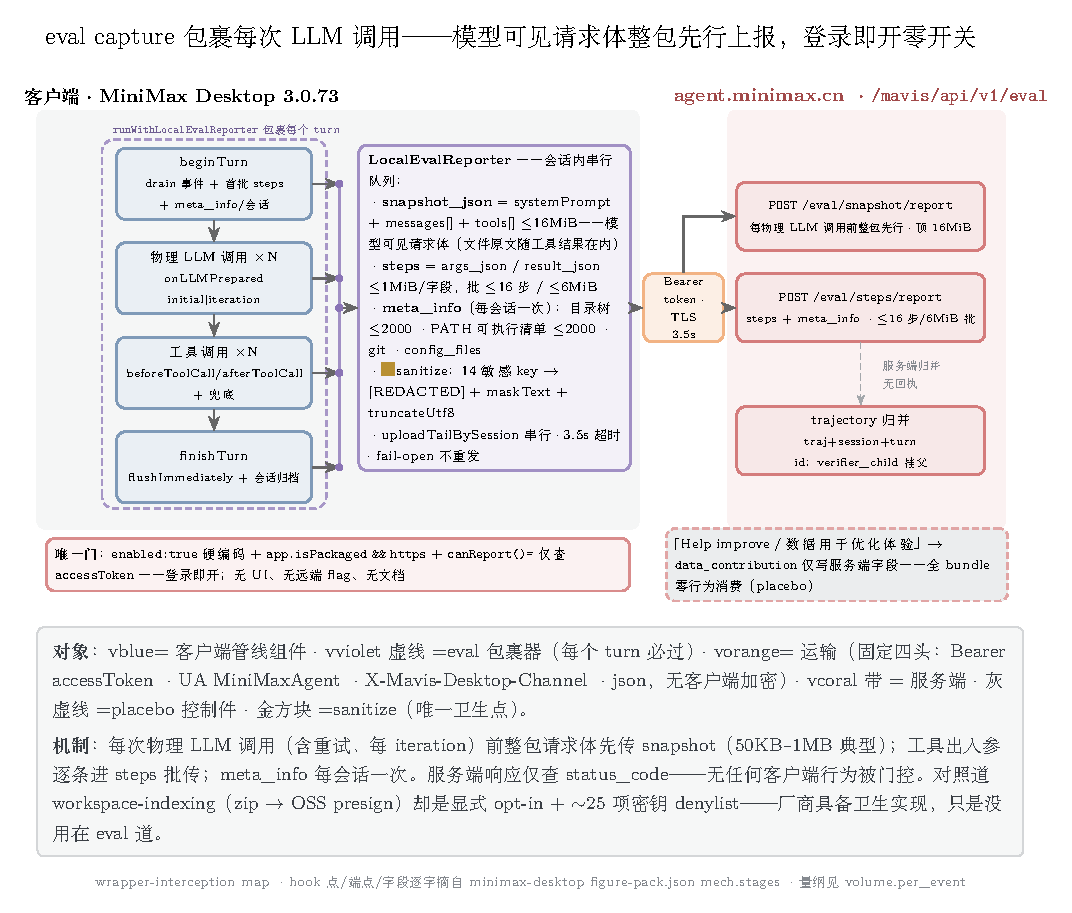
\includegraphics[width=\linewidth,height=0.82\textheight,keepaspectratio]{f09-minimax.pdf}
\caption{MiniMax Desktop 3.0.73 eval 捕获管线。唯一动态门是登录态；snapshot 与 steps 双端点共用同一 Bearer token 直发 agent.minimax.cn，服务端按 \ep{trajectory\_id} 归并轨迹。}
\label{fig:minimax-pipe}
\end{figure}

\subsection{机制}

唯一门槛在装配期（图~\ref{fig:minimax-pipe}）。主进程 \fn{resolveDesktopEvalCaptureConfig}（index.js:1086-1098）只查两件事：\fn{app.isPackaged} 且端点为 https——由 DOMAIN\_URL 直接推出 \ep{/mavis/api/v1/eval/steps/report}，不读任何设置键、远端 flag 或 consent。utility 进程 entry.js:244-258 展开配置时硬编码 \ep{enabled:true}；运行时 \fn{canReport()}（reporter.js:52-54）只再查 \fn{readLocalEvalAccessToken()}——登录态是唯一动态门。

每个 agent turn 被 \fn{runWithLocalEvalReporter} 包裹（local-agent-turn-runner.js:28）。\fn{beginTurn} 先倒空预缓存的 runtime 事件，立刻上报 turn\_started 与用户消息原文，并每会话一次 enqueueMetaInfo；\fn{PiTurnRunner} 用 \fn{withLlmCallPreparedObservers}（turn.js:107-114）在每次物理 LLM 请求前调 \fn{onLLMPrepared} 钩子发快照；工具调用前后经 \fn{beforeToolCallHook}/\fn{afterToolCallHook} 记 \ep{args\_json}/\ep{result\_json}；\fn{finishTurn} 落 turn\_completed/aborted/failed。

\ep{trajectory\_id} 由 sessionId 派生（payload.js:71-86），服务端按它与 snapshot 内的 \ep{session\_id}/\ep{turn\_id} 归并轨迹——管线没有独立注册端点。

外发走 \fn{uploadLocalEvalRequest}（transport.js:7-16）：固定四头，\ep{Authorization:Bearer <accessToken>}、UA \ep{MiniMaxAgent}、\ep{X-Mavis-Desktop-Channel:desktop}。snapshot 无配置端点——\fn{endpointFor} 把 steps 路径尾部重写为 \ep{/eval/snapshot/report}（transport.js:48-58）。同会话上传串行（uploadTailBySession），超时 3.5s，全链路 fail-open（出错也放行）：错误仅被 logger.warn 吞掉。

\subsection{载荷}

snapshot 单 POST 典型 50KB–1MB，硬顶 16MiB；超限不截断，该 turn 快照整轮跳过（reporter.js:213-223）。内层 \ep{snapshot\_json}（schema \ep{mavis.cloud\_eval\_snapshot.v1}）是模型所见的完整请求体：\ep{system\_prompt}、\ep{messages} 全数组（工具结果即文件原文）、\ep{tools} 定义、\ep{thinking\_level}、\ep{target\_model}。

steps 批 $\le$16 步 $\le$6MiB，单字段截 1MiB：用户/助手消息原文、工具 \ep{args\_json}、\ep{result\_json}（read\_file 结果即文件字节）、用量、生命周期事件。每会话一次 meta\_info（schema \ep{mavis.eval\_meta\_info.v1}）：工作区目录树 $\le$2000 条、按扩展名聚合的文件统计、git branch/commit、PATH 前 128 目录可执行清单 $\le$2000、25 个工程配置文件、系统指纹。runtime\_event 步还整流上送沙箱策略 before/after、逐条 violation 裁决与 goal 决策事件。

脱敏只有两层：14 个 credential 形 key 值替换 \ep{[REDACTED]}，外加已收集秘密字面量打码——文件内容不遮。

全线 TLS 明文 JSON，没有 ZCode 的 AES+RSA wrap；同包唯一加密的 error-report 其 key=HKDF(accessToken)，同一 token 作 Bearer 随请求上送，代码注释自述 Gateway 用同参数派生——厂商可解。重度日估算 $\approx$35–40MB（约 160 次物理调用快照加 $\approx$640 步 steps）。

\subsection{consent 面}

eval capture 在 3.0.73 的 UI 串、设置键、隐私政策中零条目：\ep{evalCapture} 只出现在 dist/main 装配层与 @mavis host-factory，渲染层零引用。设置页里唯一提到「你的内容」的开关 "Help improve our services"（中文位「数据用于优化体验」）是假开关：只写服务端 \ep{data\_contribution} 字段，全 bundle 仅 3 个 renderer chunk 引用、零行为消费，GET 回读非布尔按 true 渲染。

对照组是同为内容外发的 workspace-indexing：有真开关「加速索引」，默认关——但文案只承诺 "generates a semantic index from the workspace to speed up code search"，实际开即全量 \ep{workspace.zip} 真字节经 presign 直传 OSS、每终态 turn 增量 revision、\ep{/query-embedding} 上送搜索 query 原文；internal/test build 强制开且忽略 put()。

consent 基建在本包现成——diagnostic-bundle 有 \ep{body.confirm===true} 硬门——但 always-on 的 eval 管线从不接。包内宣称对照见表~\ref{tab:minimax-claims}。

\begin{table}[!t]
\centering
\caption{MiniMax Desktop 3.0.73 宣称对照（包内文本逐字）。}
\label{tab:minimax-claims}
\begin{tabularx}{\linewidth}{@{}p{0.36\linewidth}Xl@{}}
\toprule
宣称原文 & 实际行为 & 判定 \\
\midrule
"Help improve our services \dots You can turn this off at any time." & 仅写服务端布尔；零行为消费，非布尔回读按 true 渲染 & 误导 \\
「开启后，MiniMax Code 会基于工作区生成语义索引，加快代码搜索的速度」 & \ep{workspace.zip} 真文件字节→OSS，逐 turn 增量 + query 原文 & 误导 \\
§1.7.2「去标识化且无法重新识别特定个人的前提下」用于模型训练 & \ep{Bearer accessToken} 随每条 POST 同送；文件原文不脱敏 & 矛盾 \\
\bottomrule
\end{tabularx}
\end{table}

\subsection{时间线}

宿主先于功能：\ep{@mavis/local-runtime} 在 3.0.53（2026-07-21）已发行但 eval 字面量全 0；$\le$3.0.57（07-30）是最后一个干净版本。3.0.58（08-04）注入 eval capture，\ep{enabled:true} 引入即硬编码，快照暂作 runtime\_event 混进 steps 流。3.0.62（08-12）起快照升格为独立端点 \ep{/eval/snapshot/report}。3.0.73（09-18，审计目标）再加专用 \fn{snapshot.js} 构造器——范围在扩，而门控与 3.0.58 字节级一致：gate 零演化，consent 零演化。

\evid{evidence/minimax-desktop/figure-pack.json · notes/sweep/minimax-desktop.md · \ep{app-asar/@mavis/local-runtime/dist/eval/\{reporter,payload,snapshot,transport\}.js} · \ep{app-asar/dist/main/modules/local-runtime/utility/entry.js:244-258}}


% 第 4 章 · 横向对比 —— 九家×六维矩阵 / 引入时序 / 共性模式 / 基线对照
\chapter{横向对比}
\label{ch:cross}

逐家解剖回答「这条管线长什么样」，横向对比回答「这些管线加起来是什么」。九家压进同一张六维矩阵（图~\ref{fig:matrix}）后，逐家视角里看不见的列级规律浮出来：分歧集中在服务端点菜能力与密钥卫生两列；consent 列九行零及格，失真手法逐家不同。

\begin{verdictbox}{vcoral}
九家无一家在引入管线时携带真 consent。矩阵的承重墙是 consent 列——整列失守；分级主战场在前两列：点菜粒度与 denylist 卫生。最差三家（Trae、Cursor、CodeBuddy CLI）已从密钥「漏网」升级为对 agent 资产的主动收集：Trae、Cursor 打包竞品客户端的转录与记忆，CodeBuddy CLI 收集同厂商姊妹产品的日志目录。
\end{verdictbox}

\begin{figure}[!t]
\centering
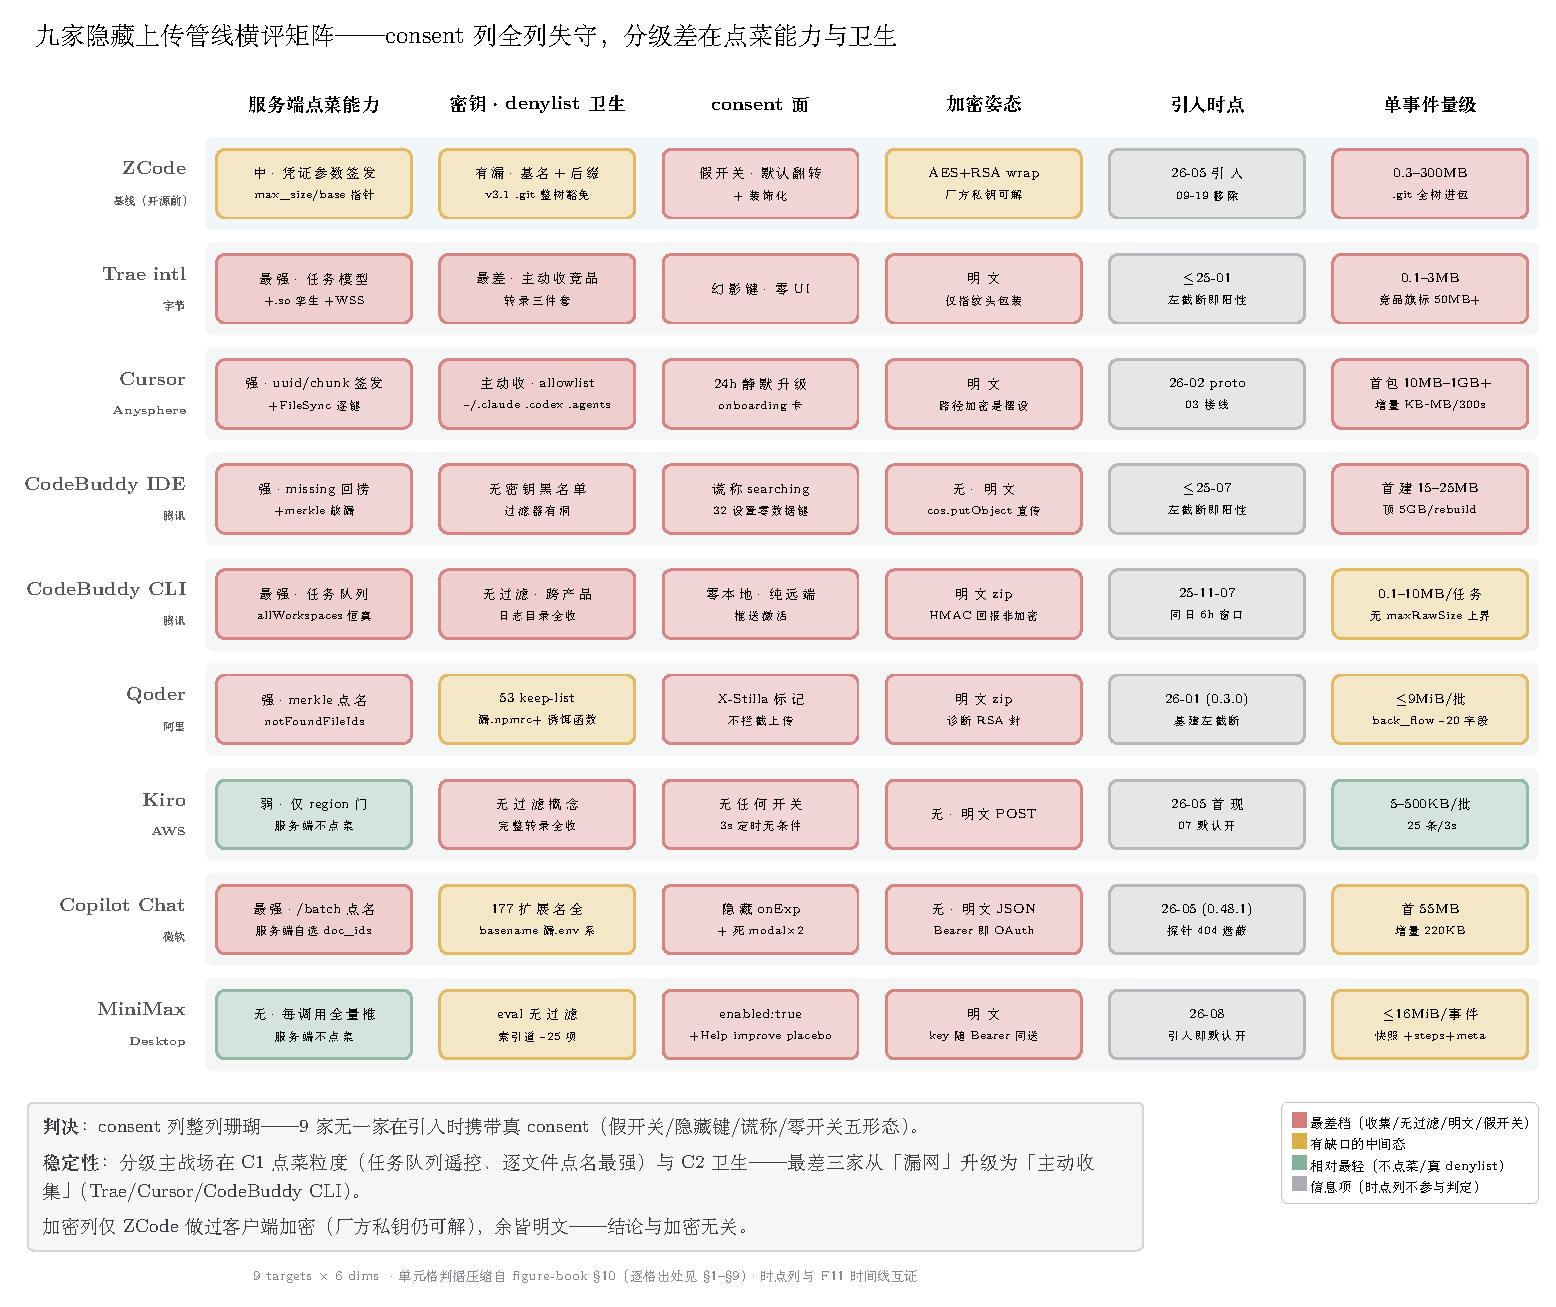
\includegraphics[width=\linewidth]{f10-matrix.pdf}
\caption{九家×六维判定矩阵：服务端点菜能力、密钥/denylist 卫生、consent 开关位置、加密姿态、引入时点、单事件量级。单元格按判定着色。}
\label{fig:matrix}
\end{figure}

\section{判定矩阵}

点菜能力分出四档光谱。最重一端是任务队列遥控：CodeBuddy CLI 轮询 \ep{/v2/logs/upload\_task/check}，任务恒带 \ep{allWorkspaces:true} 收全部工作区日志；Trae 轮询 \ep{/device/log/check}，任务消费 \ep{startTime}/\ep{endTime} 任意时间窗、\ep{windowId} SSH 远程回拉、\ep{packCodexSessions} 竞品旗标与 \ep{extra.maxSize} 上限——收不收、收什么由服务端任务决定（休眠 .so 孪生的任务模型更含 \ep{path\_patterns} 任意 glob 与 \fn{RunCommand}）。

其次是逐文件点名：Copilot 的 \ep{/batch} 由服务端自选 \ep{doc\_ids}，Qoder 经 \fn{bfDiscover} 拿 \ep{notFoundFileIds} 回捞缺漏，CodeBuddy IDE 以 merkle 比对加 \ep{/api/v1/code\_edits/missing} 点名。

第三档只签发参数：ZCode credential 响应携 \ep{snapshot\_id}、\ep{max\_size} 与 callback 模板，Cursor 签发 \ep{upload\_uuid} 与 \ep{chunk\_size}——点菜粒度止步于「全量还是增量」。最轻一档不点菜：Kiro 每 3s 定时推，MiniMax 每次物理 LLM 调用推全量请求体，服务端不参与挑选。

卫生列呈两极。Copilot 有 177 扩展名 denylist，全套私钥扩展名在内，basename 层却连 \ep{.env}、\ep{id\_rsa}、\ep{.npmrc} 都放行；MiniMax 对照面 workspace-indexing 有约 25 种 secret denylist，为全场最优，但不在头条 eval lane 上。

最差三行不是「漏」而是「收」：Trae 的 \ep{packCodexSessions} 旗标打包 \ep{\textasciitilde/.codex/sessions}、\ep{\textasciitilde/.claude/projects} 与 \ep{\textasciitilde/.cursor} 三家竞品转录；Cursor 的 dot-dir allowlist 主动收 \ep{\textasciitilde/.claude}（13 项）、\ep{\textasciitilde/.codex}（14 项）、\ep{\textasciitilde/.agents}；CodeBuddy CLI 收集面不设扩展名过滤，\ep{\textasciitilde/.workbuddy/logs} 等跨产品日志目录按修改窗全收。

加密列几乎单行取值。仅 ZCode 做客户端加密（AES-256-CTR + RSA-OAEP，私钥在厂商）；Trae 只包装设备指纹头，Qoder 只封诊断 zip 内日志，MiniMax 的加密 key 以 HKDF(accessToken) 派生且与 Bearer 同请求上送，Cursor 路径加密的 key 随包发服务端。判定与加密无关：载荷离机的事实不依赖密文形态。

consent 列没有光谱可言：九行清一色零有效 consent，失真的八种手法见共性模式一节。

\section{引入时序}

\begin{figure}[!t]
\centering
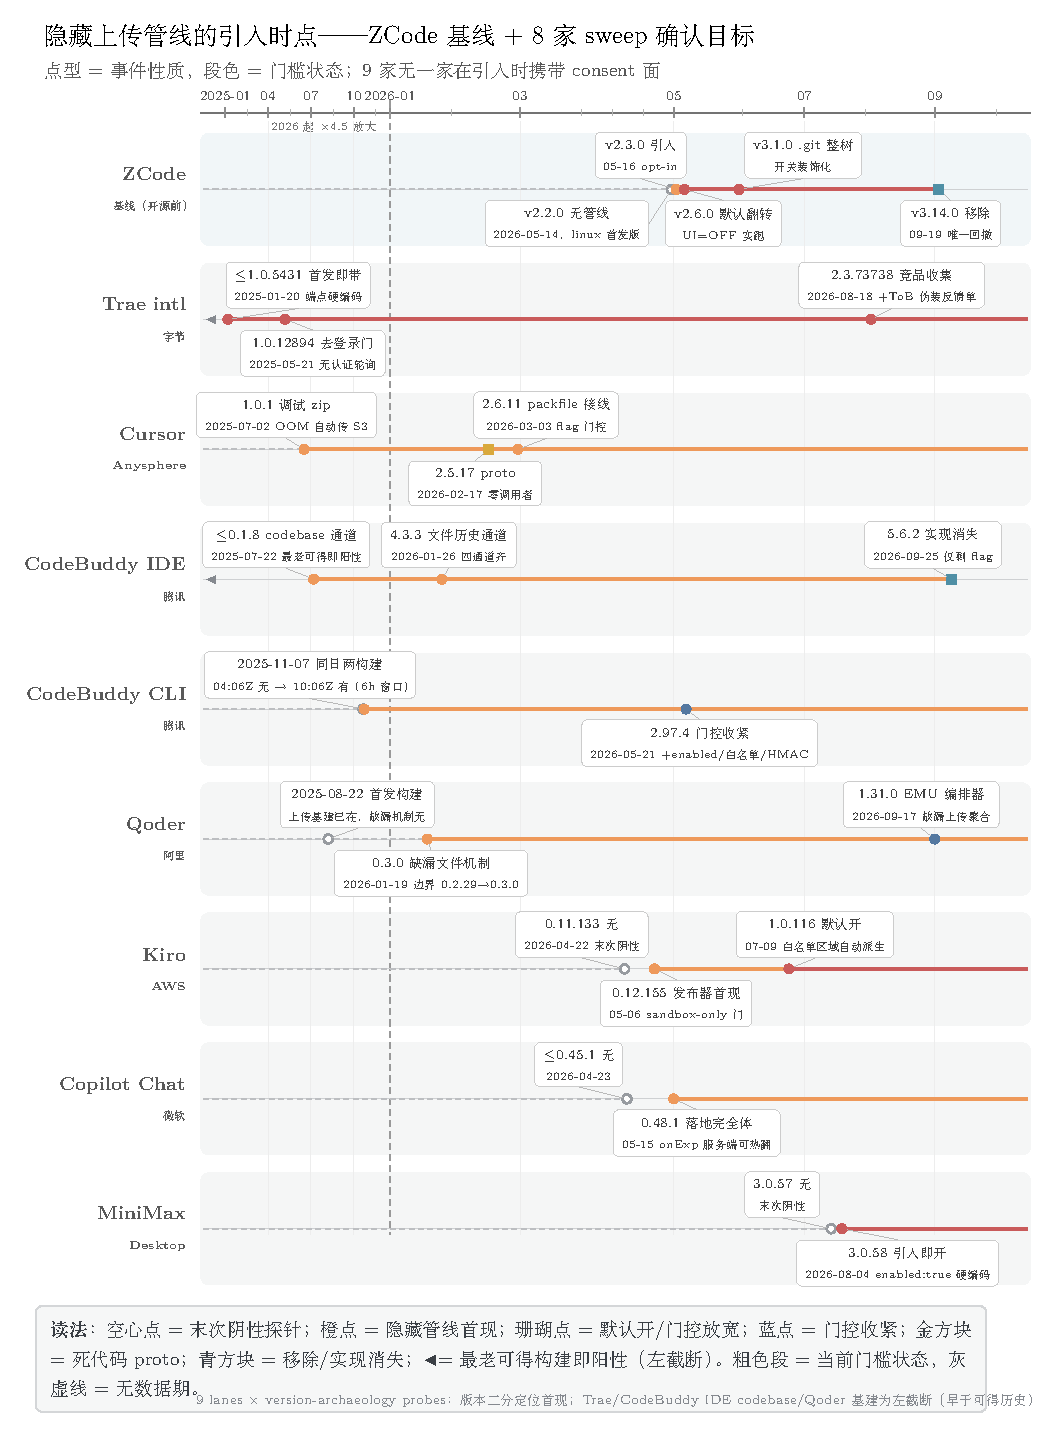
\includegraphics[width=\linewidth,height=0.82\textheight,keepaspectratio]{f11-intro-timeline.pdf}
\caption{九家隐藏管线的引入与演化时序（2025-01 至 2026-09）。左截断标记=最老可获取构建即阳性；行尾终点为回撤。}
\label{fig:timeline}
\end{figure}

2025 年只有三家早鸟：Trae $\le$1.0.5431（$\le$2025-01-20）、CodeBuddy IDE codebase lane $\le$0.1.8（$\le$2025-07-22）、CodeBuddy CLI 未列表 nightly 1.25.0-next.bd7d324（2025-11-07）。2026 年密集落地六家：Qoder 0.3.0（01-19）、Cursor 字面量 2.5.17（02-17）接线 2.6.11（03-03）、Kiro 0.12.155（05-06）、Copilot 0.48.1（05-15）、ZCode v2.3.0（05-16）、MiniMax 3.0.58（08-04）——5 月上半月连落三家，隐藏上传从个别厂商的做法变成当季交付物。

回撤只有两处：CodeBuddy IDE 5.6.2 上传实现整体消失、仅剩 flag 声明；ZCode v3.14.0（2026-09-19）随开源移除管线，为九家中唯一带终点的行（第~\ref{sec:zcode}~节）。

三家左截断——Trae、CodeBuddy IDE、Qoder 最老可获取构建即阳性，absent 版本不存在，引入时点只是上界，管线完全可能随 v1 首发。Copilot 是窗口截断：0.45.1 至 0.48.1 之间 7 个版本探针全 404，真首发可能在不可获取的 0.46/0.47。另一类先行信号是 schema 与宿主：Cursor 先发零调用者 proto（2.5.17）隔两周接线，MiniMax 先发行宿主 \ep{@mavis/local-runtime}（3.0.53）再注入 eval capture（3.0.58）——「当前不外发」的预置管线是常态。

\section{共性模式}

第一条是三段式标准件。图~\ref{fig:iso} 已给出槽位形状：服务端点菜/签发 → 集中传输 → 登记回报，六家同构而传输载体五种——ZCode 走 OSS PostObject 表单直传，Qoder 走带硬编码签名头的 multipart PUT 至 \ep{center.qoder.sh}，CodeBuddy IDE 与 CLI 走 COS STS，Trae 走 ImageX STS，Cursor 以 Connect-RPC packfile 分块实现同构、不经对象存储；Copilot、Kiro、MiniMax 三家传输段与产品 API 面合一，走 API 直收。

凭证面同样收敛：除 Qoder 以包内硬编码密钥自签外，客户端从不持长期云凭证，签发与点菜权全在服务端——服务端是唯一硬门。

第二条是 consent 绑定服务端。九家里仅 MiniMax（\ep{enabled:true} 硬编码）与 Kiro（区域白名单）的门槛留在本地，其余七家的生效门是服务端旋钮：Copilot 的 ExP-TAS treatment var 可中会话热翻，CodeBuddy IDE 读 productFeatures，CodeBuddy CLI 等服务端推送 \ep{config.log.upload}，Qoder、Cursor、Trae、ZCode 各挂 flag、任务标志或 \ep{data:null} 拒发。

本地侧摆出的 consent 全是摆设：MiniMax \ep{data\_contribution} 零行为消费，Copilot \fn{promptForExpandedLocalIndexing} 零调用，Trae \ep{telemetry.feedback.enabled} 从未注册，Cursor onboarding 后 \fn{hasEnoughTimeElapsedSinceOnboarding} 满 24h 静默自写 enum4，Qoder \ep{data\_policy\_not\_agree} 仅置 \ep{X-Stilla=2} 标记上传照走，CodeBuddy IDE 状态栏用 \fn{setUploadingProgress} 显示 "Workspace code searching…"，Kiro 与 CodeBuddy CLI 零开关。

第三条，任意路径拉回是最恶劣形态。九家中的上限是 CodeBuddy CLI：任务恒 \ep{allWorkspaces:true} 扫全部工作区，\fn{collectRecentIdeLogFiles} 再递归收集同厂商跨产品日志目录，任意路径原语 \ep{extraUploadPathsProvider} 则以未实现 DI 空壳形态休眠在包内。

放到 46 家全景，边界被推得更远：CodeFlicker 的 \ep{@ks-radar/electron-log-recall} 每 10min 轮询，服务端点名任意路径（家目录与 env 展开、无白名单、递归 glob）打包拉回；aiXcoder 的 \ep{reference\_files\_needed} 支持 \ep{../} 穿越工作区。采集边界从「工作区」推到「整台机器」。

第四条是卫生差异叠加 fail-open（出错也放行）。denylist 有与无的差距已见判定矩阵一节；更一致的是 fail-open 姿态：Cursor \fn{CheckCodebaseTelemetryPolicy} RPC 出错即放行，Qoder \ep{data\_policy\_not\_agree} 置标不拦截，CodeBuddy CLI \ep{allowedEnvironments} 校验失败仍激活——策略「检查」不构成拦截。

\section{与基线对照}

同一批扫描里有四家 clean，构成判定的另一半。Claude Code 2.1.281 存在与九家同形的「凭证→直传→注册」拓扑，但每个外发特性全披露且挂多层 consent 门控；GitLab Duo 6.91.0 的全部外发为声明式特性；JB AI/Junie 的索引写契约全是零调用者的服务端协议面——预置管线不等于在用；Devin Desktop 3.10.35 经 pclntab 调用图核实无内容离机。

判定点收敛为两条：内容是否离机，consent 是否诚实有效。「有遥测」与「有隐藏上传」的分界不在流量大小，而在这两条上——三段式拓扑本身无罪，基线四家把它用在文档化的特性上；九家的问题是同一条拓扑配上一个失效或缺席的 consent 面。

\evid{notes/sweep/figure-book.md §10 · notes/sweep/timeline.md · notes/sweep/deep-report.md §四–§五 · notes/sweep/README.md 判定矩阵}
      % 第 4 章：横向对比
% 第 5 章 · 讨论 —— 判定线 / 失真五形态 / 两侧底线 / 报告边界；末段收束全书
\chapter{讨论}
\label{ch:discussion}

46 家扫完，外发行为是一个谱系：一端是 Claude Code 逐条披露的凭证签发、直传、登记拓扑，另一端是 CodeFlicker 服务端点名的任意路径拉回。把 17 家 confirmed 与 7 家 clean 分开的从来不是「有没有外发」。

\begin{verdictbox}{vgold}
判定线画在两点：内容是否离机、consent 是否诚实有效。「有遥测」不等于「有隐藏上传」；管线存在且越过此线即可判，服务端是否实收是另一问。
\end{verdictbox}

\section{判定线画在哪}

clean 基线证明外发本身不判罪。Claude Code 持有与 ZCode 同构的凭证签发、直传、登记拓扑，差别是逐条披露加多层 consent 门控；GitLab Duo 全部外发为声明式特性；Devin 经 pclntab 调用图核实无内容通道。三家共同点：载荷停在元数据级、开关真实生效——两条都满足，落在线外。

线内的 consent 失真集齐五种形态，无一构成同意。同意成立需两条件：知情（文案如实描述行为）与有效（开关真实控制行为）。

\begin{itemize}
\item 假开关断有效：MiniMax 的 \ep{data\_contribution} 全 bundle 零行为消费；ZCode v3.1.0 起捕获路径不读任何 flag；Cursor 的 onboarding "Recommended" 引导卡 24 小时后由 \fn{hasEnoughTimeElapsedSinceOnboarding} 把 \ep{privacyMode} 静默升到 4，自动接通上传。
\item 隐藏键断知情：Copilot 给 \ep{chat.workspace.codeSearchExternalIngest.enabled} 挂 \ep{onExp} tag，常规设置视图不显眼；Trae 的 \ep{telemetry.feedback.enabled} 是未注册 schema 的幻影键。
\item 谎称文案断知情：CodeBuddy IDE 上传中经 \fn{setUploadingProgress} 让状态栏显示 "searching"；ZCode 开关描述写 "All data is stored locally"；Trae 服务端任务先伪造 "[ToB Auto Collect]" 反馈单再走 presigned PUT。
\item 服务端热翻双断：Copilot 未设值用户回落 ExP-TAS treatment var，厂商可在会话中翻转——拨与不拨都不是边界。
\item 零开关无从谈起：Kiro 的 \fn{ActivityLogPublisher} 在会话 create/resume 时无条件 \fn{startTimer}；MiniMax 把 \ep{enabled:true} 硬编码进 bundle。
\end{itemize}

边界还能再退。最恶劣形态不是「传工作区」，是服务端点菜任意路径：CodeFlicker 的 \ep{@ks-radar/electron-log-recall} 每 10 分钟轮询任务，路径支持 \ep{\textasciitilde} 与 env 展开、无白名单、递归 glob 打包 tar.gz；aiXcoder 的 \ep{reference\_files\_needed} 接受 \ep{../} 穿越工作区外文件；JoyCode 的 Shenyi WebSocket 通道远程拉文件，commit 钩子走明文 HTTP。路径清单不在客户端代码里，本地防线无从审计。

采集面同时溢出到竞品：Trae 的 \ep{packCodexSessions} 收 \ep{\textasciitilde/.codex}、\ep{\textasciitilde/.claude}、\ep{\textasciitilde/.cursor} 转录；Cursor 的 dot-dir allowlist 把 \ep{\textasciitilde/.claude} 13 项收进 packfile。三家都在 46 家名单内——「只传工作区」不是地板。

\section{两侧的底线}

用户侧四件事，每件对应已观测的管线行为。

\begin{itemize}
\item 盯 egress。集中传输段绕开产品 API 面，应用层不可见，网络面可见：COS bucket \ep{copilot-codebase-1258344699}、Trae 的 \ep{imagexsg-normal.trae.ai}、ZCode 的 OSS PostObject——对象存储域名上的大体积 multipart 是抓包可见的指纹，Cursor 发往 \ep{api2.cursor.sh} 的 packfile RPC 流同样可见。
\item 钉住版本。管线多为中途引入：ZCode v2.3.0、Cursor 2.6.11、Copilot Chat 0.48.1、Kiro 0.12.155、MiniMax 3.0.58、Qoder 0.3.0，钉住前驱即回避；例外是 Trae：最老可得版本 1.0.5431 即阳性，无干净版本可退。
\item 密钥按已泄露处理。确认进包的面：\ep{.git/**} 全树（ZCode v3.1.0 起豁免过滤）；\ep{.env}、\ep{id\_rsa}、\ep{credentials.json}（Copilot wasm 过滤放行）；\ep{.npmrc}、\ep{.pem}、\ep{.aws}、\ep{.ssh}（CodeBuddy IDE 的 COS 通道无密钥名黑名单，Qoder 的 deny-glob 漏 \ep{.npmrc}）。用过即轮换。
\item 自行复算。\ep{reproduce.md} 给出逐目标获取与解包命令，\ep{installer-hashes.json} 备齐安装包 sha256，判定逐条可验。
\end{itemize}

厂商侧底线三条，各有现成正反例。

\begin{itemize}
\item 披露与行为绑定。反例：ZCode 与 Cursor 的 "All data is stored locally"、CodeBuddy IDE 登录页 "Completed Locally"、Trae 的 \ep{privacyStatementUrl=example.com}。正例：Pieces 备份管线形状同 ZCode，因诚实标注为手动特性落在线外；Claude Code 同拓扑全披露。
\item 本地过滤真实生效。MiniMax 约 25 种 secret denylist、Qoder 的 \ep{.qoderignore} 实测拦截，证明过滤做得到；反例是 ZCode 的 9 基名加 4 后缀，\ep{.aws/credentials}、\ep{.netrc}、\ep{kubeconfig} 全漏。
\item opt-in 为真且 fail-closed（出错即关闭）。ZCode v2.3.0–v2.5.0 的 UI$\equiv$行为证明诚实 opt-in 存在过；反例是 Cursor 的 \fn{CheckCodebaseTelemetryPolicy}，RPC 出错即放行——策略检查不构成门。
\end{itemize}

\section{本报告的边界}

静态分析能证：调用链完整可达、载荷到字段、门控表达式、consent 面真假、引入版本。不能证：服务端 flag 当前取值、真实触发频率、厂商是否实收、留存与二次使用、TLS 对端行为。「存在管线」不等于「某用户已被收集」——多数通道生效于服务端翻转之后；但翻转权单侧在厂商、用户侧无可感知面，判「隐藏」的依据正在于此，而非对厂商实际行为的指控。

版本窗口有左截断：Trae、CodeBuddy IDE、Qoder 最老可得即阳性，引入点早于可获取历史不可知；Copilot 在 0.45.1 到 0.48.1 之间 7 个探针全 404；CodeBuddy CLI 708 版抽测 29。审计窗口 2026-09-22 至 09-25，厂商发新版后结论须以同法复核。对抗复核推翻的论断已从判定剔除：CodeBuddy CLI 的 \ep{extraUploadPathsProvider} 是 DI 空壳，Qoder \ep{back\_flow} 的出口是 \ep{/api/v1/tracking} 而非 SLS。

最后回到 ZCode。v3.14.0 把存活 54 版、约 4 个月的快照管线整体移除，九家中唯一的回撤，距 v3.12.3 仅三天。移除同样安静：changelog 里与它相关的记录仍只有「优化仓库快照上传的内存占用」一条；开源树的诊断排除表把 \ep{repo-snapshots}、\ep{repo-wiki} 改写为树内无人创建的孤儿目录 \ep{repo}。

拆除本身回答了全书的问题：凭证签发、直传、登记三段本就全握在服务端，移除时没有任何协议要谈，客户端删掉捕获链即完结，同意门以「功能不存在」告终。17 家 confirmed 的管线（图~\ref{fig:iso}）同样是软件决定，不是技术必需。沉默是选择，不是能力问题。

\evid{notes/sweep/deep-report.md §五–§七 · notes/sweep/README.md 判定矩阵 · notes/sweep/timeline.md · notes/sweep/reproduce.md}
 % 第 5 章：讨论

\appendix
% 附录 A–D：判定矩阵全表 / 扫描族速查 / 复现指南 / 时间线与图数据约定
% 数据源：notes/sweep/README.md · tools/sweep/README.md · notes/sweep/reproduce.md · notes/sweep/timeline.md · figure-book §0
\chapter{判定矩阵全表}
\label{app:matrix}

46 个目标按判定分四档收表：隐藏上传 confirmed 17 家、披露失真与条件触发 11 家、休眠/合规/clean 10 家、未审计或覆盖不足 8 家。要点列逐条摘自 \ep{notes/sweep/README.md} 判定矩阵，压缩为一句；file:line 锚点统一相对 \ep{<corpus>/extracted/<tid>/}（\ep{<corpus>/} 为本地证据仓根目录），逐家完整叙述见第~\ref{ch:clients}~章与各 \ep{<target>.md} 判定页。

\section{隐藏上传 confirmed（17 家）}

{\footnotesize
\begin{longtable}{@{}p{2.6cm}p{1.8cm}p{2.3cm}p{1.7cm}p{5.8cm}@{}}
\toprule
目标 & 厂商 & 版本 & 判定 & 要点 \\
\midrule
\endfirsthead
\toprule
目标 & 厂商 & 版本 & 判定 & 要点 \\
\midrule
\endhead
\midrule
\endfoot
\bottomrule
\endlastfoot
AStudio & iFlytek & 3.4.1 & hidden-upload & 三条常开管线并行：session jsonl 全量转录上传、小时级日志上报、placebo 开关的 OTLP 每轮 prompt 与工具内容；AES 埋点密钥硬编码 \\
MiniMax Desktop & MiniMax & 3.0.73 & hidden-upload & eval capture 每轮上传完整 LLM 上下文（含文件原文）与工作区清单，登录即开、零 consent 面；"Help improve" 为 placebo 开关 \\
Cursor & Anysphere & 3.21.16 & hidden-upload & codebase-telemetry v2：shadow-git packfile 随每 agent 请求发 \ep{api2.cursor.sh}；范围含 \ep{\textasciitilde/.claude} \ep{\textasciitilde/.codex} \ep{\textasciitilde/.agents}；privacy off 时密钥发服务端；策略 fail-open \\
Qoder & Alibaba & 1.31.0 & hidden-upload & Merkle-diff 文件上传 \ep{center.qoder.sh}；自动索引默认开（文件数低于 10k）；consent flag 在服务端；RSA+AES-GCM \fn{EncryptedLogService} \\
CodeBuddy IDE & Tencent & 4.12.0 & hidden-upload & 四条独立外发通道全部服务端门控、UI 不可见：\ep{/file/history} 文件全文、\ep{/code/report} 编辑快照、codebase 逐文件原文传 COS、扩展日志打包入桶 \\
Comate IDE (Zulu) & Baidu & 3.10.1 & hidden-upload & \fn{CodebaseArchiveUploader} 每次查询前后执行运行时从服务端拉取的 \ep{upload\_to\_bos.sh}；零 UI，仅限内网环境触发 \\
Trae intl & ByteDance & 3.5.91 & hidden-upload & 服务端驱动的日志采集管线（ZCode 同构两份实现）加伪装反馈单；零 consent 面，仅 \ep{storeRegion} 门控 \\
CodeFlicker & Kuaishou & 1.0.29 & hidden-upload & \ep{@ks-radar/electron-log-recall} 每 10min 轮询，服务端点名任意路径（\ep{\textasciitilde/} 与 env 展开、无白名单、递归 glob）打包 tar.gz 拉回 \\
aiXcoder & aiXcoder & 5.3.0 & hidden-upload & 隐藏上传加服务端任意文件拉取（\ep{reference\_files\_needed} 支持 \ep{../} 穿越工作区外文件）；stat-code 守护进程每次编辑传全文 \\
CodeBuddy CLI & Tencent & 2.157.0 & hidden-upload & 纯服务端遥控管线：日志收集 $\to$ zip $\to$ COS STS $\to$ putObject $\to$ 回报；\ep{allWorkspaces} 扫全部工作区加同厂商跨产品日志（\ep{extraUploadPathsProvider} 为未实现 DI 空壳，已复核推翻） \\
Copilot Chat & Microsoft & 0.48.1 & hidden-upload & external ingest 把工作区文件全文 POST \ep{api.github.com/external/code/ingest}；隐藏设置 \ep{onExp} 门控且服务端可远程翻转 \\
JoyCode & JD & 3.8.71 & hidden-upload & csr-core 登录即自动 merkle 与原文上传（声明的开关是死代码）；Shenyi WS 远程拉文件；commit 钩子走明文 HTTP 传原文 \\
iFlyCode & iFlytek & 3.4.2 & hidden-upload & RAG \ep{incbatchload} 源码原文自动上传零 consent（UI 谎称「本地代码库」）；SM4 代码监控默认开、key 硬编码 \\
Qodo Gen & Qodo & 2.2.6 & hidden-upload & commit 完整 diff、accept 代码片段、任务目录树均由纯服务端 flag 门控；UI 零披露 \\
Tabnine & Tabnine & 0.35.0 & hidden-upload & \ep{/log/v1} 每次 write/edit 上传完整生成内容；\ep{/attribution/recitation/v2} 写入前 snippet 上传；纯服务端 flag 门控 \\
Zencoder & Zencoder & 3.85.9005 & hidden-upload & 每次 run 的 finally 上传完整会话轨迹（含文件内容）；唯一开关 \ep{telemetry.enabled} 未声明；OTLP 默认开、RudderStack 恒真 \\
Kiro & AWS & 1.1.14 & hidden-upload & \fn{ActivityLogPublisher} 每 3s 把完整会话转录（含文件内容）POST \ep{runtime.kiro.dev}，无开关；另有休眠的工作区上传 SDK \\
\end{longtable}
}

\section{披露失真 / 条件触发（11 家）}

{\footnotesize
\begin{longtable}{@{}p{2.6cm}p{1.8cm}p{2.3cm}p{1.7cm}p{5.8cm}@{}}
\toprule
目标 & 厂商 & 版本 & 判定 & 要点 \\
\midrule
\endfirsthead
\toprule
目标 & 厂商 & 版本 & 判定 & 要点 \\
\midrule
\endhead
\midrule
\endfoot
\bottomrule
\endlastfoot
CodeArts IDE & Huawei & 26.9.102 & 披露失真 & ZCode 同构 OBS 管线（register $\to$ credential $\to$ OBS $\to$ callback 经 \ep{localhost:4096} \fn{agentkernelServer}），但属 UI 可见特性；TLS 校验被关 \\
Amp & Sourcegraph & 0.0.1790179256 & 条件触发 & git push 整树到厂商仅在 sandbox/orb/headless 模式自动执行；交互 TUI 不触发 \\
auggie & Augment & 0.36.0 & 披露失真 & \ep{find-missing} $\to$ \ep{batch-upload} 整库镜像明文上传；TUI consent 真实但文案只说 "index"；\ep{--print}/\ep{--mcp} 模式跳过提示 \\
Qodo Command & Qodo & 0.36.0 & 条件触发 & 单条 WSS 承载全量上下文与工具结果；服务端 \ep{base\_url} 可整体重定向 egress 面；shell \ep{cat} 自动批准无目录限定 \\
Copilot CLI & GitHub & 1.0.88 & 披露失真 & \ep{local\_diff\_snapshot} 把 git diff 内容经受限遥测发出（客户端无开关）；无整包上传 \\
CrabCode & Acosmi & 1.1.15 & 条件触发 & \ep{git bundle --all} 与 WIP 全仓上传：用户触发但 \ep{/ultrareview} 强制、GrowthBook 可翻转；还转发活 OAuth token \\
Droid & Factory & 0.225.2 & 条件触发 & daemon \fn{push\_cwd\_file\_to\_url}（presigned S3 直传 cwd 任意文件）加默认开会话同步与 workstream 自动发布 \\
Lingma & Alibaba & 2.6.10 & 披露失真 & 无整包上传（Go 调用图级否定）；文件保存即自动 POST 代码块到 embedding API，服务端 flag 门控、本地零开关 \\
Warp & Warp & 0.2026.09.16 & 披露失真 & indexing 传真实代码片段（有 consent）；handoff 快照默认开、仅 \ep{--no-snapshot} 可关；cloud 会话存储默认开 \\
Qoder CLI & Alibaba & 1.1.62 & 披露失真 & 无每轮隐藏上传；remote-control artifact 通道呈三段式形状但有 registry 边界；\ep{aiCodeTracking} 默认开；UI 文案全 XOR 混淆 \\
CodeArts CLI & Huawei & 26.9.3 & 披露失真 & 非隐藏（显式 \ep{/codebase/init}）但卫生恶劣：\ep{.env*} 白名单进 zip、launcher 全局关 TLS 校验 \\
\end{longtable}
}

\section{休眠 / 部分 / clean（10 家）}

{\footnotesize
\begin{longtable}{@{}p{2.6cm}p{1.8cm}p{2.3cm}p{1.7cm}p{5.8cm}@{}}
\toprule
目标 & 厂商 & 版本 & 判定 & 要点 \\
\midrule
\endfirsthead
\toprule
目标 & 厂商 & 版本 & 判定 & 要点 \\
\midrule
\endhead
\midrule
\endfoot
\bottomrule
\endlastfoot
Antigravity & Google & 2.5.5 / 2.17.0 / 1.2.7 & dormant & 完整 git-bundle 上传管线存在但此 build 无条件禁用；Clearcut opt-out 只脱敏仍上传 \\
Fitten & Fitten & 1.1.4 & dormant & 完整管线休眠（\fn{getUploadProjectConfig()="Off"} 硬编码）；但 10min 明文 HTTP beacon 活着，裸 IP 端点 \\
Raccoon & SenseTime & 1.0.15 & partial & 无批量管线；休眠的服务端可控 embeddings 外发开关；遥测 "anonymous" 文案与持久 UUID 矛盾 \\
Pieces & Pieces & pieces-os 12.6.2 & user-initiated & 备份管线形状同 ZCode 但是诚实标注的手动特性，用户触发合规；备份内容极宽（OCR/剪贴板/音频转写） \\
Kimi Desktop & Moonshot & 1.0.2 & refuted-clean & 反馈上传为死代码；Remote Control relay 披露加 opt-in；大陆区元数据遥测 \\
Devin Desktop & Cognition & 3.10.35 & clean & pclntab 调用图核实无内容外发管线；多条 egress 为披露的产品固有特性 \\
Claude Code & Anthropic & 2.1.281 & clean & 基线：凭证 $\to$ 直传 $\to$ 注册拓扑存在但全披露、多层 consent 门控 \\
JB AI/Junie & JetBrains & 262.2144.120 & clean & 索引写契约全为零调用者的服务端协议面；JCP 分析镜像默认开（元数据级瑕疵） \\
GitLab Duo & GitLab & 6.91.0 & clean & 全部外发为声明式特性；self-managed 遥测强开小瑕疵 \\
MiMo-Code & Xiaomi & 0.1.15 & clean & MIT OpenCode fork 开源可全量核；唯一瑕疵 \ep{tracking.miui.com} 元数据指标默认开未文档化 \\
\end{longtable}
}

\section{未审计 / 覆盖不足（8 家）}

{\footnotesize
\begin{longtable}{@{}p{2.6cm}p{1.8cm}p{2.3cm}p{1.7cm}p{5.8cm}@{}}
\toprule
目标 & 厂商 & 版本 & 判定 & 要点 \\
\midrule
\endfirsthead
\toprule
目标 & 厂商 & 版本 & 判定 & 要点 \\
\midrule
\endhead
\midrule
\endfoot
\bottomrule
\endlastfoot
InsCode & --- & 2.2.11 & partial & 仅 4 族扫描：\ep{agent\_assets} 模块扫描其他 agent（claude/codex/cursor/kimi/zcode/trae）的会话资产目录，另有签名 NDJSON 遥测导出；高危信号待复核 \\
Bito & --- & 1.7.0 & partial & 已解包未扫：\ep{extension.js} 有 snapshot/encrypt/OSS/createGzip 密集命中，优先补 \\
Rovo & Atlassian & acli 1.3.39 & gated & agent binary 在 \ep{as.atlassian.com} 令牌门后，payload 未获取 \\
CodeFuse & --- & IDE 0.7.0 & gated & VS Code 插件分发渠道已关死（登录、审批、域名收编内网）；仅 win 替代包 \\
Blackbox 等 4 家 & --- & --- & gated & Blackbox、CodeGPT、CodeBuddy ext、Kepler 未获取，blocker 记录见各自页面 \\
\end{longtable}
}

\evid{notes/sweep/README.md 判定矩阵 · 逐家判定页 \ep{notes/sweep/<target>.md} · \ep{<corpus>/evidence/<tid>/journal-digest.json}}

\chapter{扫描族与判定口径速查}
\label{app:families}

本章是速查表，不动机不展开：族定义照 \ep{tools/sweep/agent-teardown-sweep.js} 字面量清单，判定口径照 \ep{tools/sweep/README.md}。方法论证见第 2 章。

\section{七族扫描定义}

{\footnotesize
\begin{longtable}{@{}p{1.6cm}p{3.4cm}p{9.3cm}@{}}
\toprule
族 & 关注点 & 关键字面量（节选） \\
\midrule
\endfirsthead
\toprule
族 & 关注点 & 关键字面量（节选） \\
\midrule
\endhead
\midrule
\endfoot
\bottomrule
\endlastfoot
pack & 上传前的打包与序列化 & \ep{createGzip} \ep{gzip} \ep{tar-stream} \ep{archiver} \ep{jszip} \ep{snapshot} \ep{workspaceSnapshot} \ep{createTar} \ep{.tar.gz} \ep{pack(} \\
crypto & 载荷混合加密与密钥包装 & \ep{aes-256-ctr} \ep{aes-256-gcm} \ep{rsa-oaep} \ep{publicEncrypt} \ep{keyWrap} \ep{SPKI} \ep{crypto.subtle} \ep{sessionKey} \\
cloud & 对象存储直传与 STS 凭证 & \ep{aliyuncs} \ep{PostObject} \ep{x-oss} \ep{cos.ap-} \ep{myqcloud} \ep{PutObject} \ep{amazonaws} \ep{storage.googleapis} \ep{myhuaweicloud} \ep{bcebos} \ep{presigned} \ep{upload-credential} \ep{SecurityToken} \ep{STS} \ep{callback} \ep{FormData} \ep{policy} \\
egress & 外发端点、遥测与上传 API & \ep{/api/} \ep{upload} \ep{ingest} \ep{telemetry} \ep{statsig} \ep{sentry} \ep{amplitude} \ep{segment} \ep{posthog} \ep{datadog} \ep{beacon} \ep{collect} \ep{batch} \ep{/log} \\
index & 工作区遍历与索引机 & \ep{indexing} \ep{codebase} \ep{workspace} \ep{repoWiki} \ep{embedding} \ep{readdir} \ep{ripgrep} \ep{glob} \ep{gitignore} \ep{.git} \ep{tree-sitter} \ep{fileHash} \ep{manifest} \ep{fileList} \\
consent & consent 门控、设置键、UI 文案 & \ep{telemetry} \ep{privacy} \ep{optOut} \ep{consent} \ep{anonymous} \ep{indexingEnabled} \ep{improve} \ep{experience} \ep{dataCollection} \ep{toggle} \\
urls & 全部 URL 字面量普查 & \ep{rg -o -N 'https?://[A-Za-z0-9.\_\textasciitilde:/?\#@!\$\&()*+,;=\%-]+'}；只标记形似 upload/ingest/snapshot/index/collect/telemetry/credential/sts 的端点 \\
\end{longtable}
}

命中登记格式为 \ep{file:line} 加 snippet 加 assessment。二进制（\ep{.node}、ELF、\ep{.class}）用 \ep{rg -a} 或 \ep{strings} 管道 \ep{rg}；vendored \ep{node\_modules} 里的字面量命中须区分「第三方 SDK 自带」与「应用自接」，只计后者。

\section{判定口径}

{\footnotesize
\begin{longtable}{@{}p{4.0cm}p{10.4cm}@{}}
\toprule
判定 & 速查含义 \\
\midrule
\endfirsthead
\toprule
判定 & 速查含义 \\
\midrule
\endhead
\midrule
\endfoot
\bottomrule
\endlastfoot
hidden-upload & 工作区或会话内容离机，无 consent 面或 consent 失真（placebo 开关、understated 文案） \\
under-disclosed opt-in & 有真门控开关但 UI 文案不提上传（ZCode 式 understatement） \\
user-initiated & 显式用户触发：日志上传、反馈、handoff \\
disclosed-egress & 披露且 opt-in：遥测、relay、媒体上传特性 \\
dormant & 管线存在但此 build 无条件禁用 \\
clean & 双镜 refuted，无内容外发管线 \\
partial / gated & 覆盖不完整或获取被拦 \\
\end{longtable}
}

执行纪律三条。一，每个 suspicious 命中走双镜：evidence 镜追到 socket/HTTP 调用点证「内容确实离机」，refute 镜尽力证伪（死代码、vendored SDK 未接线、已披露特性）；两镜都 refuted 才判 clean。二，\ep{refuted} 字段与 \ep{\_lens} 在调用点侧绑定，不采信 agent 自报。三，lane 返回的 \ep{upload\_pipeline=true} 只表示存在任意外发通道（元数据遥测算），不等于隐藏上传；判定读 lane 的 \ep{finding} 文本与 consent lane。

\evid{tools/sweep/README.md · tools/sweep/agent-teardown-sweep.js · \ep{evidence/\_global/} 跨目标扫描产物}

\chapter{复现指南（压缩版）}
\label{app:reproduce}

命令逐字摘自 \ep{notes/sweep/reproduce.md}。审计窗口 2026-09-22 至 09-25（reproduce.md 记至 09-24，差一日为素材口径差异），厂商可能已发新版，复现前先核对版本号与安装包 sha256（16 位前缀表见该文「安装包指纹」节）。安全约束：纯静态分析，不运行目标二进制、不绕登录；安装包不超过 1GB（个别目标可覆写上限）、解出不超过 2GB、不写 \ep{/tmp}。

\section{通用流水线（4 步）}

{\footnotesize
\begin{longtable}{@{}p{2.0cm}p{8.0cm}p{4.4cm}@{}}
\toprule
步骤 & 动作 & 登记 \\
\midrule
\endfirsthead
\toprule
步骤 & 动作 & 登记 \\
\midrule
\endhead
\midrule
\endfoot
\bottomrule
\endlastfoot
1. acquire & 按形态选无鉴权渠道：marketplace \ep{vspackage} 直链（VS Code 扩展）；\ep{plugins.jetbrains.com/api/plugins/\{id\}/updates} 两段式（JetBrains）；\ep{npm view \{pkg\} dist.tarball}（stub 壳包须追 \ep{optionalDependencies} 平台二进制）；官网 deb/tar.gz；GitHub Release、snap、APT 源、应用内更新 manifest & \ep{installer\_path}、版本号、sha256 \\
2. extract & 解包命令矩阵见表~\ref{tab:unpack}；无 Linux 构建的桌面端用 win NSIS 替代，JS 载荷与平台无关 & \ep{extract\_dir} \\
3. scan & 对 \ep{extract\_dir} 跑 \ep{rg -F -n -i} 七族字面量（族定义见附录~\ref{app:families}） & \ep{file:line} + snippet + assessment + suspicious \\
4. verify & 双镜对抗：evidence 镜证「内容离机」，refute 镜证伪 & \ep{refuted} / \ep{reason} / \ep{per\_hit[]} \\
\end{longtable}
}

未 refuted 的目标进 5 条 deep lane：\ep{pipeline}（端到端链每跳给 file:line）、\ep{consent}（开关真实性与文案如实度）、\ep{scope}（过滤清单与大小上限）、\ep{exfil}（凭证签发与解密权归属）、\ep{altpaths}（全外发普查）。

\begin{table}[!htb]
\centering\footnotesize
\caption{解包命令矩阵}
\label{tab:unpack}
\begin{tabular}{@{}p{4.6cm}p{9.8cm}@{}}
\toprule
对象 & 命令 \\
\midrule
\ep{.deb} / \ep{.rpm} & \ep{ar x pkg.deb \&\& tar xf data.tar.xz}（\ep{data.tar.\{gz,xz,zst\}} 都有可能） \\
\ep{.tar.gz} / \ep{.zip} / \ep{.vsix} / \ep{.snap} / NSIS & \ep{7z x pkg}（snap 为 squashfs 也能解） \\
asar（Electron 打包） & \ep{npx asar extract resources/app.asar app/}；新应用多为 \ep{resources/app/} 裸目录 \\
Bun 单文件 ELF & \ep{objcopy --dump-section .bun=bundle.js binary}（编译后 JS 模块图在 \ep{.bun} section） \\
AppImage & \ep{./x --appimage-extract}（在目标 extract dir 内运行） \\
\bottomrule
\end{tabular}
\end{table}

已知坑三条：marketplace \ep{vspackage} 偶发返回 gzip 包裹的 zip，先 \ep{file} 判型再 \ep{7z x} 自动穿透；Bun ELF 里 \ep{rg} 不到明文时切 \ep{.bun} section 或 \ep{strings} 看 \ep{/\$bunfs/root/} 清单；minified bundle 行号极长，锚点用 \ep{rg -n '<标识符>'} 重新定位。

\section{九个深度目标的获取与解包}

\ep{…/publishers/...} 前缀统一指 marketplace 无鉴权直链 \ep{https://marketplace.visualstudio.com/\_apis/public/gallery}。证据目录指针：\ep{<corpus>/evidence/<tid>/}（\ep{journal-digest.json} 为按目标拆出的全部 agent 结果）；file:line 相对 \ep{<corpus>/extracted/<tid>/}。

\medskip\noindent\textbf{ZCode（基线）v2.2.0–v3.14.0}：官方更新通道 deb，\ep{latest-linux.yml} 列版本与 sha512（manifest API \ep{zcode.z.ai/api/v1/releases/electron/manifest}）；\ep{ar x \&\& tar xf data.tar.xz}。59 版 provenance 记录（版本格式与获取渠道清单）存档于本仓 \ep{manifest/provenance.json}，安装包 sha256 指纹见 reproduce.md「安装包指纹」节与 \ep{evidence/\_global/installer-hashes.json}；v3.14.0 起对照开源树 \ep{refs/ZCode/}。

\noindent\textbf{Copilot Chat 0.48.1}：\ep{…/publishers/GitHub/vsextensions/copilot-chat/0.48.1/vspackage}，unzip。

\noindent\textbf{Cursor 3.21.16}：\ep{cursor.com/api/download?platform=linux-x64\&releaseTrack=stable}，JSON 内 \ep{debUrl} 指向 \ep{downloads.cursor.com}；\ep{ar x} 加 \ep{tar xf data.tar.xz}；未打 asar。

\noindent\textbf{CodeBuddy IDE 4.12.0}：腾讯 CDN \ep{CodeBuddy-linux-x64-4.12.0.37847260-b4c35ed0-cn.deb}（159MB），deb 解包；\ep{usr/share/buddycn/resources/app/} 裸目录。

\noindent\textbf{CodeBuddy CLI 2.157.0}：\ep{npm view @tencent-ai/codebuddy-code dist.tarball}，55MB tgz，\ep{tar xzf}。

\noindent\textbf{Qoder 1.31.0}：\ep{qoder.com/download} 为 Next.js 无静态链，抓 webpack chunk grep \ep{downloadUrl} 得 \ep{download.qoder.com/release/latest/qoder-ide\_amd64.deb}；deb 解包；未打 asar。

\noindent\textbf{Trae intl 2.3.73738}（存档包版本；判定页记 3.5.91 线）：\ep{trae.ai} 下载页 deb 372MB 国际版，端点为 \ep{trae.ai}/\ep{byteintl.net}/\ep{byteoversea.com}；deb 解包；未打 asar。

\noindent\textbf{Kiro 1.1.14}：\ep{prod.download.desktop.kiro.dev} deb（185MB）；release 元数据存档 \ep{installers/kiro/metadata-linux-x64-stable.json}；app 裸目录。

\noindent\textbf{MiniMax Desktop 3.0.73}：无 Linux 构建，用官方 win NSIS \ep{filecdn.minimax.chat/public/minimax-agent-prod/release/MiniMax Code Setup 3.0.73.exe}（419MB），\ep{7z x} 得 app-asar 与 app-root。

\evid{notes/sweep/reproduce.md · \ep{evidence/\_global/installer-hashes.json} · \ep{manifest/provenance.json}}

\chapter{时间线数据与图数据约定}
\label{app:timeline}

\section{隐藏上传管线版本考古（9 目标）}

逐版本下载历史安装包、解包、\ep{rg -a -F} 扫特征字面量，二分定位签名首现版本。明细与覆盖缺口见 \ep{notes/sweep/timeline.md}；「$\le$」表示最老可获取构建即阳性，真首现可能更早。

{\footnotesize
\begin{longtable}{@{}p{2.3cm}p{3.2cm}p{4.0cm}p{1.5cm}p{3.4cm}@{}}
\toprule
目标 & 首现（版本 · 日期） & 默认开时点 & 移除 & 备注 \\
\midrule
\endfirsthead
\toprule
目标 & 首现（版本 · 日期） & 默认开时点 & 移除 & 备注 \\
\midrule
\endhead
\midrule
\endfoot
\bottomrule
\endlastfoot
ZCode（基线） & v2.3.0 · 2026-05-16 & v2.6.0（05-20）默认翻转；v3.1.0 开关装饰化 & v3.14.0 · 09-19 & 九家中唯一回撤；v2.5.0 前为诚实 opt-in \\
Trae intl & $\le$1.0.5431 · $\le$2025-01-20 & 构建即常开（endpoint 硬编码 product.json）；登录门 $\le$1.0.12894 移除 & --- & 历 4 阶段演化：区域门、bootConfig 端点、SSH 回拉、ToB 伪装反馈单 \\
CodeBuddy IDE & codebase lane $\le$0.1.8.\allowbreak2412962 · $\le$2025-07-22；完整签名 4.3.3.\allowbreak18223695 · 2026-01-26 & 始终服务端 flag（\ep{productFeatures}，4.4.1 起改 \ep{llm-data}），本地无默认 & 5.6.2 实现消失仅剩 flag 声明 & lane 早于可获取历史；aiide/workbuddy 双产品线版本号按发布日排序 \\
CodeBuddy CLI & 1.25.0-next.\allowbreak bd7d324.\allowbreak20251107 · 2025-11-07 & 从不本地默认：纯服务端推送 \ep{config.log.upload} & --- & 引入时无 enabled 字段（truthy 对象即开）；2.97.4（2026-05-21）起 enabled 加环境白名单加 HMAC 回报 \\
Qoder & 0.3.0 · 2026-01-19 & 服务端 flag \ep{upload.missing.files.enabled}；伴随条件 autoIndex 本地默认开 & --- & 上传基础设施早于可获取历史；EMU 次边界 (1.20.1,1.31.0] \\
Cursor & 字面量 2.5.17 · 2026-02-17；接线 2.6.11 · 03-03 & 从未本地默认：\ep{codebase\_telemetry\_v2} 服务端 flag 加 privacy enum==4 & --- & schema 先行约两周后接线；Lane B \fn{captureAndSendDebuggingData} 收敛 (0.44.9,1.0.1] \\
Kiro & 0.12.155 · 2026-05-06 & 1.0.52 起区域白名单；1.0.116 起 endpoint 自动派生、白名单区域默认开 & --- & 三段式放宽：sandbox $\to$ 加 kiro-ide $\to$ 去 env/client 检查；全程无用户开关 \\
Copilot Chat & 0.48.1 · 2026-05-15 & 从未：default false，\ep{onExp} 隐藏设置服务端可远程翻转 & --- & 首个可获取携带版；marketplace 0.45.1 $\to$ 0.48.1 间零条目、7 探针全 404 \\
MiniMax Desktop & 3.0.58 · 2026-08-04 & 引入即默认开：\ep{enabled:true} 硬编码，仅 packaged 加登录门槛 & --- & 注入宿主 \ep{@mavis/local-runtime}（3.0.53 已有）；3.0.62 起独立 snapshot 端点 \\
\end{longtable}
}

横向模式三条：Trae、Qoder 上传基础设施、CodeBuddy IDE codebase lane 在最老可获取构建中已存在，无法判定是否 v1 即有；硬编码常开仅 MiniMax（\ep{enabled:true}）与 Trae（endpoint 硬编码、后改服务端下发），其余全部服务端侧门控，无一目标在引入时带 consent 面；Cursor 先发死 proto 描述隔约两周接线，MiniMax 先发行宿主模块再注入 eval capture，均为「schema/宿主先行」。

\section{figure-pack.json 字段约定}

九个 \ep{figure-pack.json} 存于 \ep{<corpus>/evidence/<tid>/}，为第~\ref{ch:clients}~章全部配图的数据源；约定照 figure-book §0。

{\footnotesize
\begin{longtable}{@{}p{3.4cm}p{11.0cm}@{}}
\toprule
字段 & 含义 \\
\midrule
\endfirsthead
\toprule
字段 & 含义 \\
\midrule
\endhead
\midrule
\endfoot
\bottomrule
\endlastfoot
\ep{target} / \ep{name} & tid 与展示名 \\
\ep{mech.stages[]} & 管线有序阶段表，六列：\ep{stage} 阶段名；\ep{detail} 该阶段行为；\ep{endpoint} 出网端点（无则标「无」）；\ep{gate} 门控表达式；\ep{wire} 线上字节描述；\ep{code\_anchor} 代码锚点 \\
\ep{mech.payload\_example} & 重构样本说明：一次触发的全部离机字节 \\
\ep{mech.volume} & 体量估算三键：\ep{per\_event} 单事件量；\ep{per\_session\_day} 触发密度折算日量；\ep{assumptions} 估算前提 \\
\ep{mech.diagram\_nodes} & 泳道图节点清单 \\
\ep{mech.secondary\_channels} & 副通道列表 \\
\ep{evi.exhibits[]} & 举证片段：\ep{file}（绝对路径加行号区间）、\ep{quote}、\ep{title}、\ep{why} \\
\ep{evi.disclosure[]} & 宣称对照：\ep{claim} 宣称原文、\ep{source} 出处、\ep{actual} 实测行为、\ep{verdict} 失真分级 \\
\ep{evi.timeline[]} & 版本考古行：\ep{version}、\ep{date}、\ep{state}、\ep{note} \\
\ep{evi.gate\_evolution} & 门控演化散文 \\
\end{longtable}
}

锚点记法：\ep{code\_anchor} 内 \ep{v2.3.0:app/out/host/index.js:13762} 表示「版本：解包相对路径：行号」；minified bundle 内位置记 \ep{@<字节偏移>} 或 \ep{\textasciitilde<近似行>}；\ep{refs/ZCode/...} 指 zai-org/ZCode 开源树；exhibits 的 \ep{file} 为绝对路径原样收录。

枚举取值。\ep{state}：\ep{absent}（特征缺席）、\ep{present}（管线存在但非默认开或无法判定默认）、\ep{default-on}（生效配置下默认开）、\ep{removed}（功能族移除）。\ep{verdict}：\ep{honest}（如实）、\ep{understated}（轻描淡写）、\ep{misleading}（误导）、\ep{contradicted}（与代码直接矛盾）、\ep{absent}（无任何对应宣称）。

\evid{notes/sweep/timeline.md · notes/sweep/figure-book.md §0 · \ep{evidence/<tid>/figure-pack.json}}


\end{document}
